%--------------------------------------------------------------------------------------
% Dokumentum formátuma [Document format]
%--------------------------------------------------------------------------------------

%TODO Válaszd ki, hogy egyoldalas vagy kétoldalas legyen! [Choose format]
%\documentclass[12pt,a4paper,oneside]{report}             % Egyoldalas [Single-side]
\documentclass[12pt,a4paper,oneside,openright]{report}  % Kétoldalas [Duplex]


%--------------------------------------------------------------------------------------
% Csomagok inicializálása [Initializing packages]
%--------------------------------------------------------------------------------------
\usepackage{ifthen} % Used in macros

\usepackage[english,magyar]{babel} % Language support
\usepackage{geometry}
\usepackage{amsfonts,amsmath,amssymb} % Mathematical symbols
\usepackage{microtype} % Imrovements to typesetting
\usepackage{setspace} % For setting line spacing
\usepackage{cmap} % Enables more advenced text copying from the PDF document 
\usepackage{sectsty} % Section heading styling

\usepackage[unicode]{hyperref} % For hyperlinks in the generated document
\usepackage{booktabs} % For publication quality tables for LaTeX
\usepackage{graphicx} % For figure sizing
\usepackage[hang]{caption}
\usepackage{xcolor} % For code coloring in listings
\usepackage{listings} % For source code snippets
\usepackage[amsmath,thmmarks]{ntheorem} % Theorem-like environments

\usepackage[numbers]{natbib} % Bibliography

% Phyl's includes
\usepackage{subcaption}
\usepackage{todonotes}
\usepackage{dirtree}
\renewcommand*\DTstylecomment{\rmfamily\color{gray}\textsc}
\renewcommand*\DTstyle{\ttfamily\textcolor{black}}
%% for notes in tables
\usepackage{marginnote}
\renewcommand{\marginpar}{\marginnote}
%% dockerfile listings
\lstdefinelanguage{Dockerfile}
{
  morekeywords={FROM, RUN, CMD, LABEL, MAINTAINER, EXPOSE, ENV, ADD, COPY,
    ENTRYPOINT, VOLUME, USER, WORKDIR, ARG, ONBUILD, STOPSIGNAL, HEALTHCHECK,
    SHELL},
  morecomment=[l]{\#},
  morestring=[b]"
}

%\usepackage{fancyhdr} % For easy to use headers and footers

% thanks to http://tex.stackexchange.com/a/47579/71109
\usepackage{ifxetex}
\usepackage{ifluatex}
\newif\ifxetexorluatex % a new conditional starts as false
\ifnum 0\ifxetex 1\fi\ifluatex 1\fi>0
   \xetexorluatextrue
\fi

\ifxetexorluatex
  \usepackage{fontspec}
  % Palatino clone font (Tex Gyre Pagella) for text and math
  \usepackage{newpxmath}
  \setmainfont[Ligatures=TeX]{TeX Gyre Pagella}
\else
  \usepackage[T1]{fontenc}
  \usepackage[utf8]{inputenc}
  %\usepackage[lighttt]{lmodern} % Advanced version of the Computer Modern font
  % Palatino clone font (Tex Gyre Pagella) for text and math
  \usepackage{tgpagella, newpxmath}
\fi



%--------------------------------------------------------------------------------------
% Dokumentum nyelve [Language]
%--------------------------------------------------------------------------------------

%TODO Válaszd ki a nyelvet! [Select language]
\input{include/language-setup-hu} % Beállítások magyar nyelvű dolgozathoz
%\input{include/language-setup-en}    % Settings for English document
https://www.overleaf.com/project/61d23b485996085245e2a939
% Megjegyzés: 
%         Ez a beállítás az automatikusan létrehozott címek, hivatkozások
%         nyelvét adja meg, valamint a nyelvre jellemző behúzási távolságot
%         használja a bekezdések elején.
%
% Note: 
%         This setting controls the language of generated titles and citations,
%         moreover the paragraph indentation.


%--------------------------------------------------------------------------------------
% Preambulum (LaTeX beállítások, makrók) [Preamble (LaTeX settings)]
%--------------------------------------------------------------------------------------
\input{include/preamble}


%--------------------------------------------------------------------------------------
% Munkatípus [Thesis type]
%--------------------------------------------------------------------------------------

%TODO Válaszd ki a munkatípust [Select thesis type]
%\selectbsc    % Szakdolgozat [Bachelor's]
\selectmsc   % Diplomaterv [Master's]


%--------------------------------------------------------------------------------------
% Változók beállítása [Setting variables]
%--------------------------------------------------------------------------------------

%TODO Állítsd be az alábbi változókat [Set these variables]

% Szerző [Author]
\def\authorFamilyName{Pelle}
\def\authorGivenName{János Fülöp}
\def\neptun{JPW0YB}

% Konzulens 1 [Consulent 1]
\def\consulentATitle{dr.~}
\def\consulentAFamilyName{Ferdinandy}
\def\consulentAGivenName{Bence}
\def\consulentARank{tudományos munkatárs}

% Konzulens 2 [Consulent 2], ha nincs hagyd üresen
\def\consulentBTitle{}
\def\consulentBFamilyName{}
\def\consulentBGivenName{}
\def\consulentBRank{}

% Konzulens 3 [Consulent 3], ha nincs hagyd üresen 
\def\consulentCTitle{}
\def\consulentCFamilyName{}
\def\consulentCGivenName{}
\def\consulentCRank{}

% Témavezető
\def\supervisorTitle{}
\def\supervisorFamilyName{Korcsok}
\def\supervisorGivenName{Beáta}
\def\supervisorRank{doktorandusz}

% Dolgozat címe [Thesis title]
\def\thesisTitle{Szemantikai információ biztosítása robotok számára korlátozott hardveren}

% Kulcsszavak (a PDF-be) [Keywords (to PDF)]
\def\keywords{mechatronika, gépi látás, etorobotika,}

% Tanszék [Department]
%TODO Válassz az alábbiak közül
% \bmeatt    \bmeara  \bmeenergia  \bmeepget  \bmegtharom 
% \bmemanuf  \bmehds  \bmemogi     \bmemm     \bmept
\def\department{\bmemogi}

%TODO Cseréld le a figures/tanszek_logo.pdf képet a tanszéked logójára!
%     [Replace figures/tanszek_logo.pdf with the logo of your department]

% Elzártan kezelendő dolgozat [Restricted access]
%TODO Töltsd ki a korlátozás lejártának dátumát! 
%     [Fill in the end date of the restriction]
\def\endOfRestrictedAccess{... év ... hónap ... nap}


% Változók beállítása a PDF fájlhoz [Apply variables for the PDF file]
\applyvariables


%--------------------------------------------------------------------------------------
% Dokumentum törzse [Document body]
%--------------------------------------------------------------------------------------

\begin{document}

\pagenumbering{gobble}
\selectthesislanguage

% Címoldal [Titlepage]
\include{include/titlepage-thesis}  % Szakdolgozat/Diplomaterv címlap [Thesis]


% Copyrightoldal [Copyright page]
%TODO Válaszd ki a megfelelőt! [Choose one]
\include{include/copyrightpage}               % Nyílt kezelésű [Open access]
%\include{include/copyrightpage-restricted}   % Elzárt kezelésű [Restricted access]


% Feladatkiírás [Project page]
%TODO A nyomtatott verzóban ne szerepeljen! [Remove before printing]
%--------------------------------------------------------------------------------------
% Feladatkiiras (a tanszeken atveheto, kinyomtatott valtozat)
%--------------------------------------------------------------------------------------
\begin{center}
\large
\textbf{FELADATKIÍRÁS}\\
\end{center}
\thispagestyle{empty}

A feladatkiírást a tanszéki adminisztrációban lehet átvenni, és a leadott munkába eredeti, tanszéki pecséttel ellátott és a tanszékvezető által aláírt lapot kell belefűzni (ezen oldal \emph{helyett}, ez az oldal csak útmutatás). Az elektronikusan feltöltött dolgozatban már nem kell beleszerkeszteni ezt a feladatkiírást.



% Nyilatkozatok [Declarations]
\include{include/declaration}

\selectthesislanguage
% Tartalomjegyzék [Table of Contents]
\setcounter{tocdepth}{3}  % Tartalomjegyzék mélysége [ToC depth]
\tableofcontents\vfill


% Ábrák és táblázatok jegyzéke [List of Figures, Tables]
%TODO Kommenteld ki, ha használni szeretnéd. [Uncomment to use]
%\listoffigures\addcontentsline{toc}{chapter}{\listfigurename}   % Ábrák jegyzéke - opcionális
%\listoftables\addcontentsline{toc}{chapter}{\listtablename}     % Táblázatok jegyzéke - opcionális


% Előszó [Preface]
%----------------------------------------------------------------------------
\chapter*{\eloszo}\addcontentsline{toc}{chapter}{\eloszo}
%----------------------------------------------------------------------------

Előszó


% Jelölések jegyzéke [Table of Symbols]
%\newcommand{\tss}{\textsuperscript}     % tss = felső index
%----------------------------------------------------------------------------
\chapter*{\jelolesek}\addcontentsline{toc}{chapter}{\jelolesek}
%----------------------------------------------------------------------------

A táblázatban a többször előforduló jelölések magyar és angol nyelvű elnevezése, 
valamint a fizikai mennyiségek esetén annak mértékegysége található. Az egyes 
mennyiségek jelölése – ahol lehetséges – megegyezik hazai és a nemzetközi 
szakirodalomban elfogadott jelölésekkel. A ritkán alkalmazott jelölések 
magyarázata első előfordulási helyüknél található.

%~~~~~~~~~~~~~~~~~~~~~~~~~~~~~~~~~~~~~~~~~~~~~~~~~~~~~~~~~~~~~~~~~~~~~~~~~~~~~~~~~~~~~
% A táblázatokat ABC rendben kell feltölteni, először mindig a kisbetűvel
% kezdve. Ha egyazon betűjelnek több értelmezése is van, akkor mindegyiket kü-
% lön sorban kell feltüntetni. Konstansok esetén az értéket is a táblázatba
% kell írni.
% Dimenzió nélküli mennyiségek mértékegysége 1 és nem: – !
% A jelölésjegyzékben csak SI vagy SI-n kívüli engedélyezett mértékegységeket
% szabad feltüntetni. Egy dokumentumon belül az SI és pl. az angolszász
% mértékrendszer nem keverhető!
%~~~~~~~~~~~~~~~~~~~~~~~~~~~~~~~~~~~~~~~~~~~~~~~~~~~~~~~~~~~~~~~~~~~~~~~~~~~~~~~~~~~~~

%~~~~~~~~~~~~~~~~~~~~~~~~~~~~~~~~~~~~~~~~~~~~~~~~~~~~~~~~~~~~~~~~~~~~~~~~~~~~~~~~~~~~~
% A Jelölés oszlop alapvetően kurzív betűváltozattal szedendő, a Mértékegység
% oszlopot álló betűkkel kell szedni. Felső indexhez használható a \tss{}
% parancs.
%~~~~~~~~~~~~~~~~~~~~~~~~~~~~~~~~~~~~~~~~~~~~~~~~~~~~~~~~~~~~~~~~~~~~~~~~~~~~~~~~~~~~~

\def\arraystretch{1.5}%  vertical cell padding

\subsubsection*{Latin betűk}
\begin{center}
    \begin{tabular}{lp{10cm}l}
        \hline
        Jelölés & Megnevezés, megjegyzés, érték & Mértékegység \\ 
        \hline
        $g$     & gravitációs gyorsulás (9.81)  & m/s\tss{2}     \\
        $p$     & nyomás                        & bar           \\
        $s$     & fajlagos entrópia             & J/(kg$\cdot$K)\\
        \hline
    \end{tabular}    
\end{center}



\subsubsection*{Görög betűk}
\begin{center}
    \begin{tabular}{lp{10cm}l}
        \hline
        Jelölés & Megnevezés, megjegyzés, érték & Mértékegység \\ 
        \hline
        $\eta$  & hatásfok                      & 1             \\      
        $\rho$  & sűrűség                       & kg/m\tss{3}    \\
        \hline
    \end{tabular}
\end{center}



\subsubsection*{Indexek, kitevők}
\begin{center}
    \begin{tabular}{lp{12.8cm}}
        \hline
        Jelölés & Megnevezés, értelmezés\\ 
        \hline
        $i$     & általános futóindex (egész szám)  \\
        nom     & névleges (nominális) érték        \\
        opt     & legkedvezőbb (optimális) érték    \\
        \hline
    \end{tabular}    
\end{center}


\def\arraystretch{1}%  vertical cell padding



% Főszöveg [The main part of the thesis]
\cleardoublepage
\pagenumbering{arabic}
%TODO Importáld a saját fejezeteidet [Import your own content]
%----------------------------------------------------------------------------
\chapter{\bevezetes}
%----------------------------------------------------------------------------

Napjaink egyik fontos problémája a robotok társadalomban elfoglalt szerepének jövőbeni alakulása. A robot szó egyik (igen tág) értelmezése olyan gép, mely automatikusan komplex\todo[color=green]{mi az az automatikus komplex?:)} feladatok ellátására képes. Ezt alapul véve a számítási kapacitás és újonnan a mesterséges intelligencia gyors fejlődésének köszönhetően számos új területen jelentek, jelennek és jelenhetnek meg. Az iparban régóta \todo{mióta?} alkalmaznak robotokat. Ezek többnyire specifikus, jól behatárolt gyártási lépésekek végeznek. Bár emberi szemszögből az ellátott feladatok nehéznek tűnhetnek pontossági igényeik, nagy ismétlésszámuk és esetleg akár az adott feladat egyes lépéseinek számát tekintve is, programozói szempontból többnyire jól behatároltak. Egy másik terület, melyen jelentős segítség és előrelépés a robotok megjelenése a katasztrófaelhárítás és mentőakciók végrehajtása. \todo{Fukushima és hasonló esetek átnézése} Az emberek számára toxikus vagy nehezen hozzáférhető területek átvizsgálására illetve az ezen területeken történő munkavégzésre nagy előrelépést jelenthet robotok alkalmazása. \todo{cikket keresni ehhez}.

Bár a szociális és a szolgáltatóipari területeken alkalmazható robotok ötlete és kutatása nem új, a hétköznapi életben manapság mégis ritkán találkozhatunk robotokkal. Az 1980-as években például nagyvállalati kereskedelmi területeken már terjedni kezdtek takarítórobotok és néhány primitívebb otthon környezetbe szánt robot is \cite{engelberger_robotics_1989}, azonban utóbbiak gyenge funkcionalitásuk miatt nem terjedtek el. A háztartásban alkalmazható robotizált porszívók fejlesztése az 1990-es években nagy népszerűségnek örvendett \cite{brittain_autonomous_1993} \cite{brutzman_beyond_1993} \cite{coombs_robovac_1993}. Az ezredfordulóra a téma extenzív irodalommal rendelkezett \cite{fiorini_cleaning_2000}. A világ első kereskedelmi forgalomban is kapható robotporszívója az Electrolux Trilobite névre keresztelt terméke, melynek első prototípusa már 1996-ban bemutatásra került.
\todo{BBC-n mutatták be, amúgy az ilyet hogyan kéne hivatkozni?}
\todo[color=green]{misc, vagy ha van onlinevide, URL}
Mégsem jelenthetjük ki, hogy napjainkra elterjedtek lennének ezen, egy sok ember számára teherként felfogott feladatot megkönnyítő szerkezetek. Ennek két oka lehet a magas költség és az otthoni szokásokból adódó környezeti adottságokhoz való alkalmazkodóképtelenség. Nem érdemes drága robotba fektetni, ha a lakás felépítése vagy a különböző akadályok (pl. szétszórt ruhák, játékok) miatt szuboptimális eredményt kapunk, melyet utána az eredetihez mérhető időbefektetéssel szükséges kijavítanunk.

A háztartások előtt érdemes lehet a szolgáltatóipartban feladatokat ellátó robotok fejlesztésével foglalkozni. Például 2010-ben irodai környezetben takarító robotokkal már jobb tisztaságot lehetett elérni némi költségemelkedés mellett.\todo[color=green]{hivatkozás!!!} Egy irodai környezet, iskola vagy egészségügyi létesítmény lényegesen rendezettebb és kontrolláltabb környezetet nyújt. Jó alapot nyújthat továbbá a szociális robotika kutatásában a vendéglátóipari megoldások fejlesztése, mely szektor az emberekkel való interakciós helyzetek biztosításán túl a pandémia óta rekord munkaerőhiányban szenved, így újonnan felerősödött piaci rést is jelenthet.
\todo{Ezt újságcikkekkel lehetne behivatkozni, azt hogyan kéne?}

Vegyünk például egy éttermi pincér robotot. Az ilyen célú szerkezet megalkotására való törekvés az ókorig visszavezethető. Az első robotok között emlegetett, Philón által leírt Automate Therapaenis egy élethű méretű szobor volt, mely az egyik kezében tartott kancsóból bort töltött amennyiben másik kezébe poharat helyeztek (\ref{fig:automaid_philon}. ábra). Bár ma ezt inkább neveznénk trükkös italautomatának, mint robotnak, hasonló szándék állt mögötte. A mesterséges intelligenciabeli\todo[color=green]{ha van időd, akkor azért az ilyen nyakatekert fogalmazásokat érdemes átnézni (meg szvsz nem is helyes az írásmód de azt nem tudom biztosan)} és hardveres korlátok miatt a magas szintű, személyre szabott felszolgálói szolgáltatások kiváltása ma még nem lehetséges.
\todo{ezt jobban kifejteni?}
Ellenben több helyen jelentek meg az emberi kapcsolatoktól elszigeteltebb megoldások, például a futószalagos kiszolgálás vagy tableten történő rendelés az asztaltól. Emellett több helyen a magas szintű kiszolgálás helyett a személyzet hiánya vagy költséghatékonyság szempontjábóll inkább csak kiadószemélyzetet alkalmaznak. Ilyen esetekben hasznos lehet robotokat alkalmazni a munkaerő kiegészítése és/vagy a szolgáltatás színvonalának növelése céljából.

\begin{figure}[h]
    \centering
    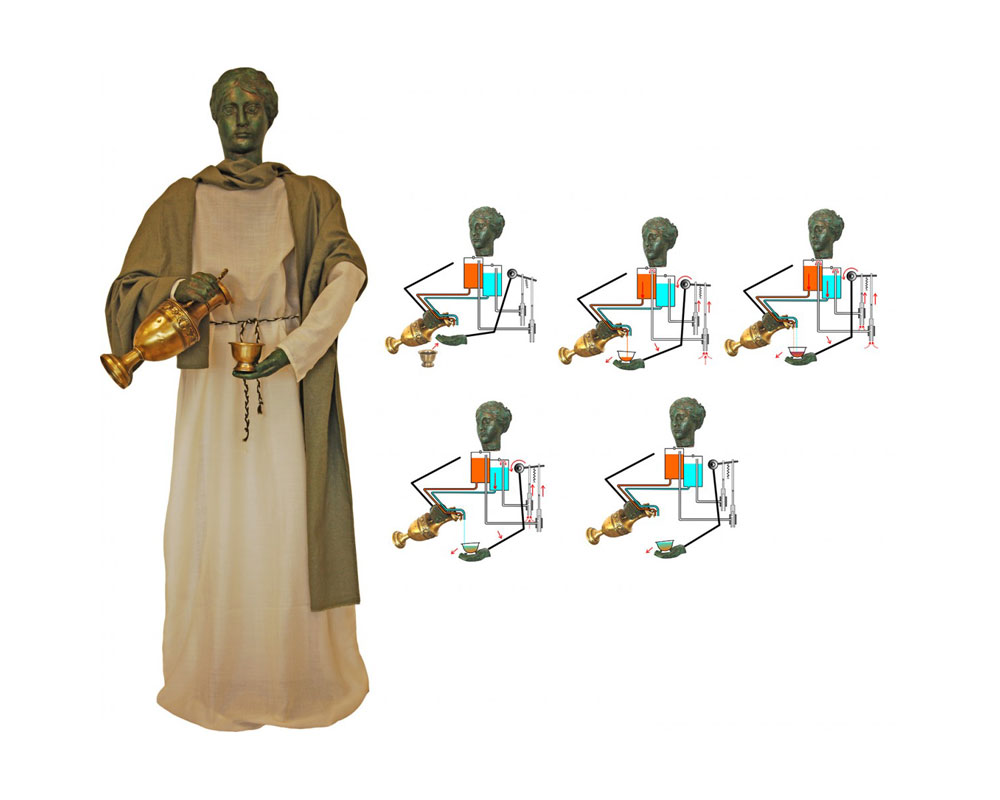
\includegraphics[width=\linewidth]{figures/automaid_philon.jpg}
    \caption{Philón automatája}
    \label{fig:automaid_philon}
\end{figure}

Az elmúlt évtizedekben növekvő figyelem irányult az emberek számára befogadható társrobotok kutatásának irányába. Sokan igyekeztek ezek közül humanoid alakkal rendelkező és humán pszichológián alapuló viselkedési mintázatokat utánozni próbáló megoldásokkal. Több kutatás is született antropomorf, érzelmeket kifejezni képes mesterséges fejek kialakításával kapcsolatban és bizonyított, hogy az emberek képesek felismerni az ezek által kifejezni kívánt érzelmeket \cite{lutkebohle_bielefeld_2010} \cite{delaunay_towards_2009} \cite{nitsch_emotions_2014}.\todo[color=green]{én nem tudom ez a template miért ilyen, de a számozott hivatkozásokat a megjelenésük sorrendjében szoktunk hivatkozni} Bár bizonyították, hogy az ezek alapján kiváltott érzelmek hasonló érzelmeket váltanak ki a valódi emberi arcok és kifejezések látványa által kiváltott érzelmekhez Chaminade és munkatársai \cite{chaminade_brain_2010} kimuattták, hogy ezek szintje és bizonyos esetekben az aktivált területek eltérést mutatnak egymáshoz képest. Az emberi interakciók és kifejezések komplexitásának és emellett az emberi agy fejlett arcfelismerő képességének köszönhetően könnyen futhatunk a modellezés során olyan kis eltérésekbe akár viselkedési mintázatokat, akár fizikai felépítést illetően, melyek negatív érzelmeket válthatnak ki. Ez a mára jól ismert "uncanny valley" (borzongások völgye) \cite{mori_bukimi_1970}.

Hasznos első lépés lehet tehát az emberi külalak és viselkedési mintázatok természetes, de ma még aligha megvalósítható vágyát elengedve alternatívák után néznünk. Az élővilág felé fordítva figyelmünket több érdekes példát is találhatunk szociális berendezkedés, kinézet és viselkedési mintázatok szempontjából is. A háziasítás során több állatfaj integrálódott az emberi életbe nem csupán haszonállatként, hanem egyéb célokra is. Legnépszerűbb példa a kutya, mely vélhetően az első háziasított faj volt. Bár régen vadászati célokat szolgált, mára legtöbben társállatként tartanak kutyát. Nem meglepő, hogy a világ második robotikus kisállata, a Sony által gyártott AIBO is kutya formájában látott napvilágot és mára negyedik generációját éli.

Külalak szempontjából érdekes betekintést biztosíthat még a számítógépes grafika, játékok és filmek világa. A filmiparban a számítógépes grafika elterjedése előtt nagymértékben alkalmaztak animatronikus modelleket. Ez ugyan mára költségessége miatt vissaszorult,\todo[color=green]{majd egy helyesírásellenőrzőt is engedj rá} ám a mai napig jelen van. Az ágazat művészei a kezdetek óta foglalkoztak azzal, hogy olyan karaktereket alkossanak meg, melyek adott érzelmeket váltanak ki. Azon túl, hogy inspirációt meríthetünk az emberek által kedvelt vonásokat illetően, megfigyelhetünk sikeres non-humanoid robotalakokat is. Nyilván ezek jó része fizikailag nem megvalósítható, azonban bizonyos elemeik átemelhetőek lehetnek a valóságba.
\todo{ábra}

\begin{figure}
    \centering
    \begin{subfigure}[b]{0.45\linewidth}
        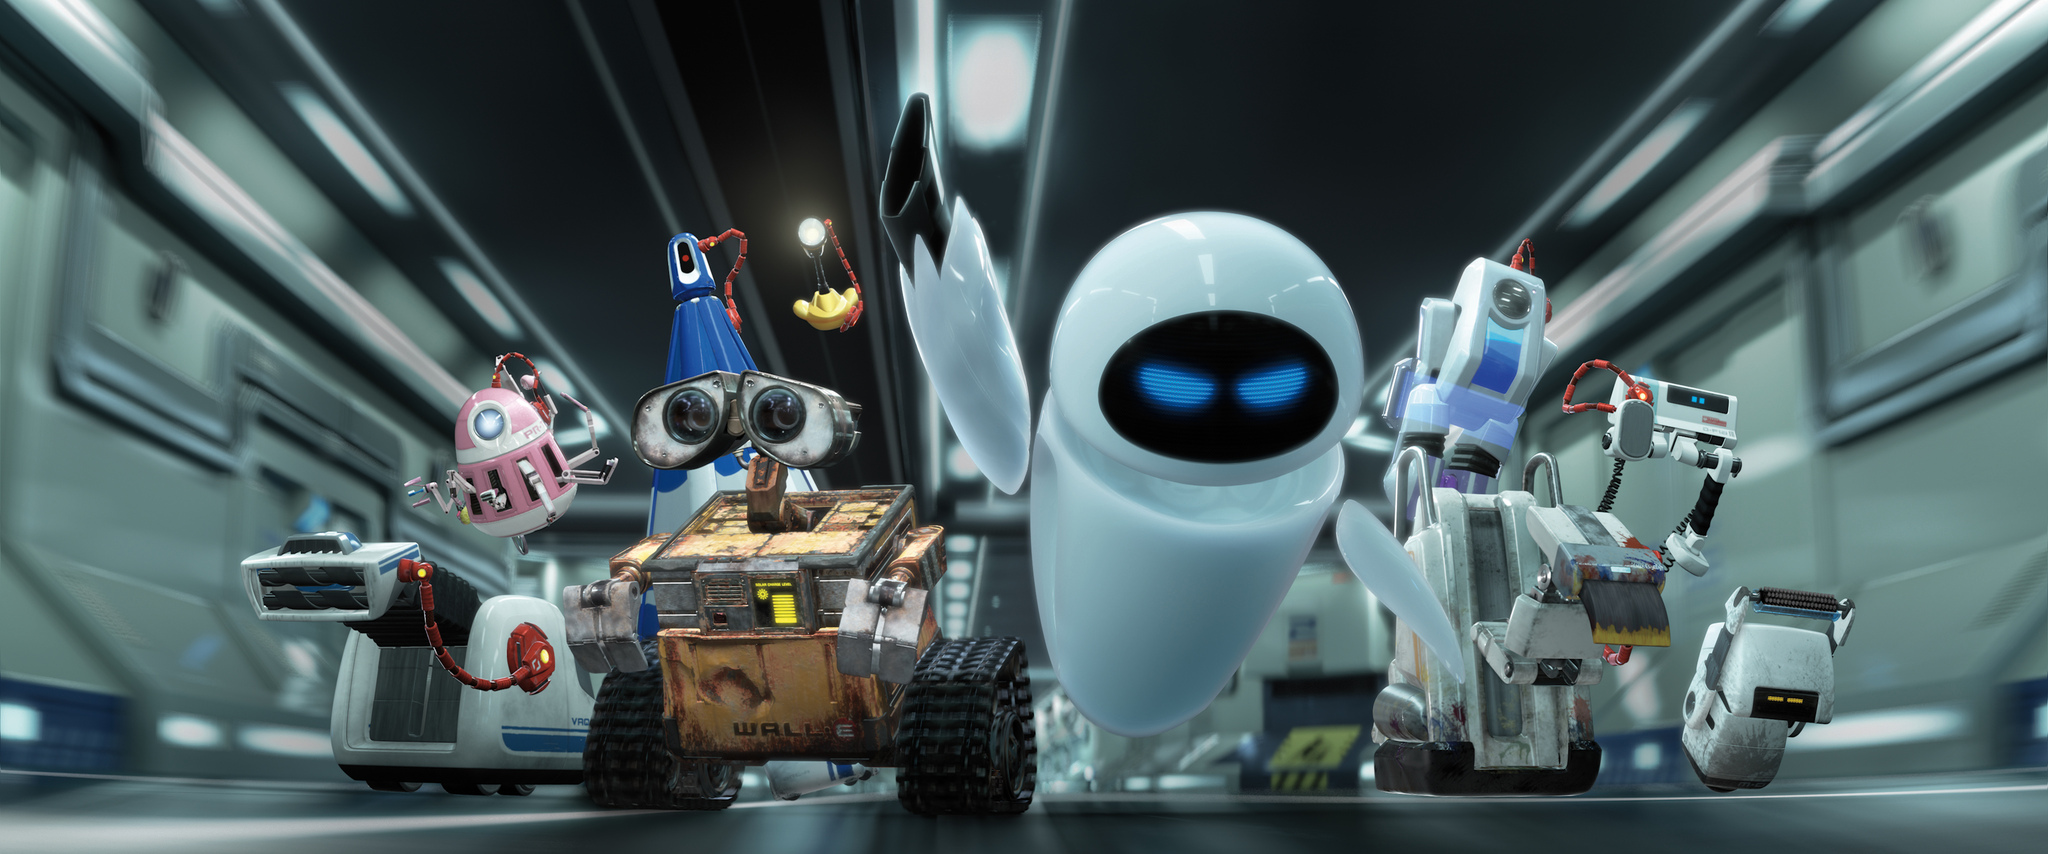
\includegraphics[height=3cm]{figures/non_humanoid_robots/wall_e.jpg}
    \end{subfigure}
    \begin{subfigure}[b]{0.15\linewidth}
        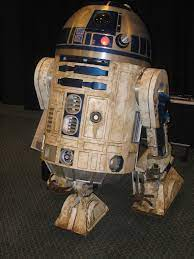
\includegraphics[height=3cm]{figures/non_humanoid_robots/r2d2.jpg}
    \end{subfigure}
    \caption{Példák non-humanoid robotokra filmekben.}
    \label{fig:neural_network_article_numbers}
\end{figure}

Fontos még, hogy a robotunk a befogadhatóságon túl feladata ellátására is képes legyen, hiszen végső soron valamilyen feladatkör elvégzésének céljából hozzuk létre. A felszolgálás feladata logisztikai és kommunikációs részekre osztható. Első lépésben a betérő látogatókat lokalizálnunk kell, majd ezt követően a rendelést valamilyen módon rögzítenünk kell. Ennek elkészülte után azt ki kell szállítanunk az asztalhoz, majd fogadnunk kell vendégeink fizetését a felszolgált tartalomért. A használt evőeszközöket ez után el kell szállítanunk bár vannak esetek, ahol ezt a vendég maga vagy külön személyzet végzi. A művelet során opcionálisan több ponton többlet kommunikációt végezhetünk a vendégekkel, de ez sem elsődleges cél. 

A navigációs és manipulációs feladatok a kereskedelmi- és gyártóipar automatizálásának köszönhetően mára megoldott feladatnak köszönhetőek. Bár az egyes cégek jellemzően nem hozzák nyilvánosságra drágán megalkotott kódbázisukat, a nyílt forráskód mozgalom népszerűségének köszönhetően mára elérhetővé váltak kedvünkre felhasználható és módosítható megoldások, melyek a fejlesztéshez szükséges időt nagymértékben csökkenthetik. Elérhetővé váltak továbbá olyan akár kereskedelmi forgalomban kapható megoldások is, melyek rugalmas alapot nyújthatnak specializáltabb kísérleti fejlesztéseknek. Ezek hozzáférhetőségét és számuk gyors növekedését segíti a Robot Operating System (Robot Operációs Rendszer, ROS) névre keresztelt szabad szoftverként fejlesztett projekt, mely nevével ellentétben nem operációs rendszerként, hanem inkább köztes kommunikációs rétegként szolgál. \todo[color=green]{pár hibát azért javítottam :)}

Hasonló gondolatok mentén és módon indult és folyik a Biscee névre keresztelt felszolgáló robot fejlesztése is az Eötvös Loránd Tudományegyetemen, mely projekthez diplomamunkám készítése során magam is becsatlakoztam. A robot alapját egy Robotnik\cite{noauthor_autonomous_nodate} RB-1 BASE mobil platform képzi, mely a(z)\todo[color=green]{majd ezeket azért nézd át hogy hova kell a, meg az}
\ref{fig:rb1_base}
. ábrán látható.
\begin{figure}
    \centering
    \begin{subfigure}[b]{0.25\linewidth}
        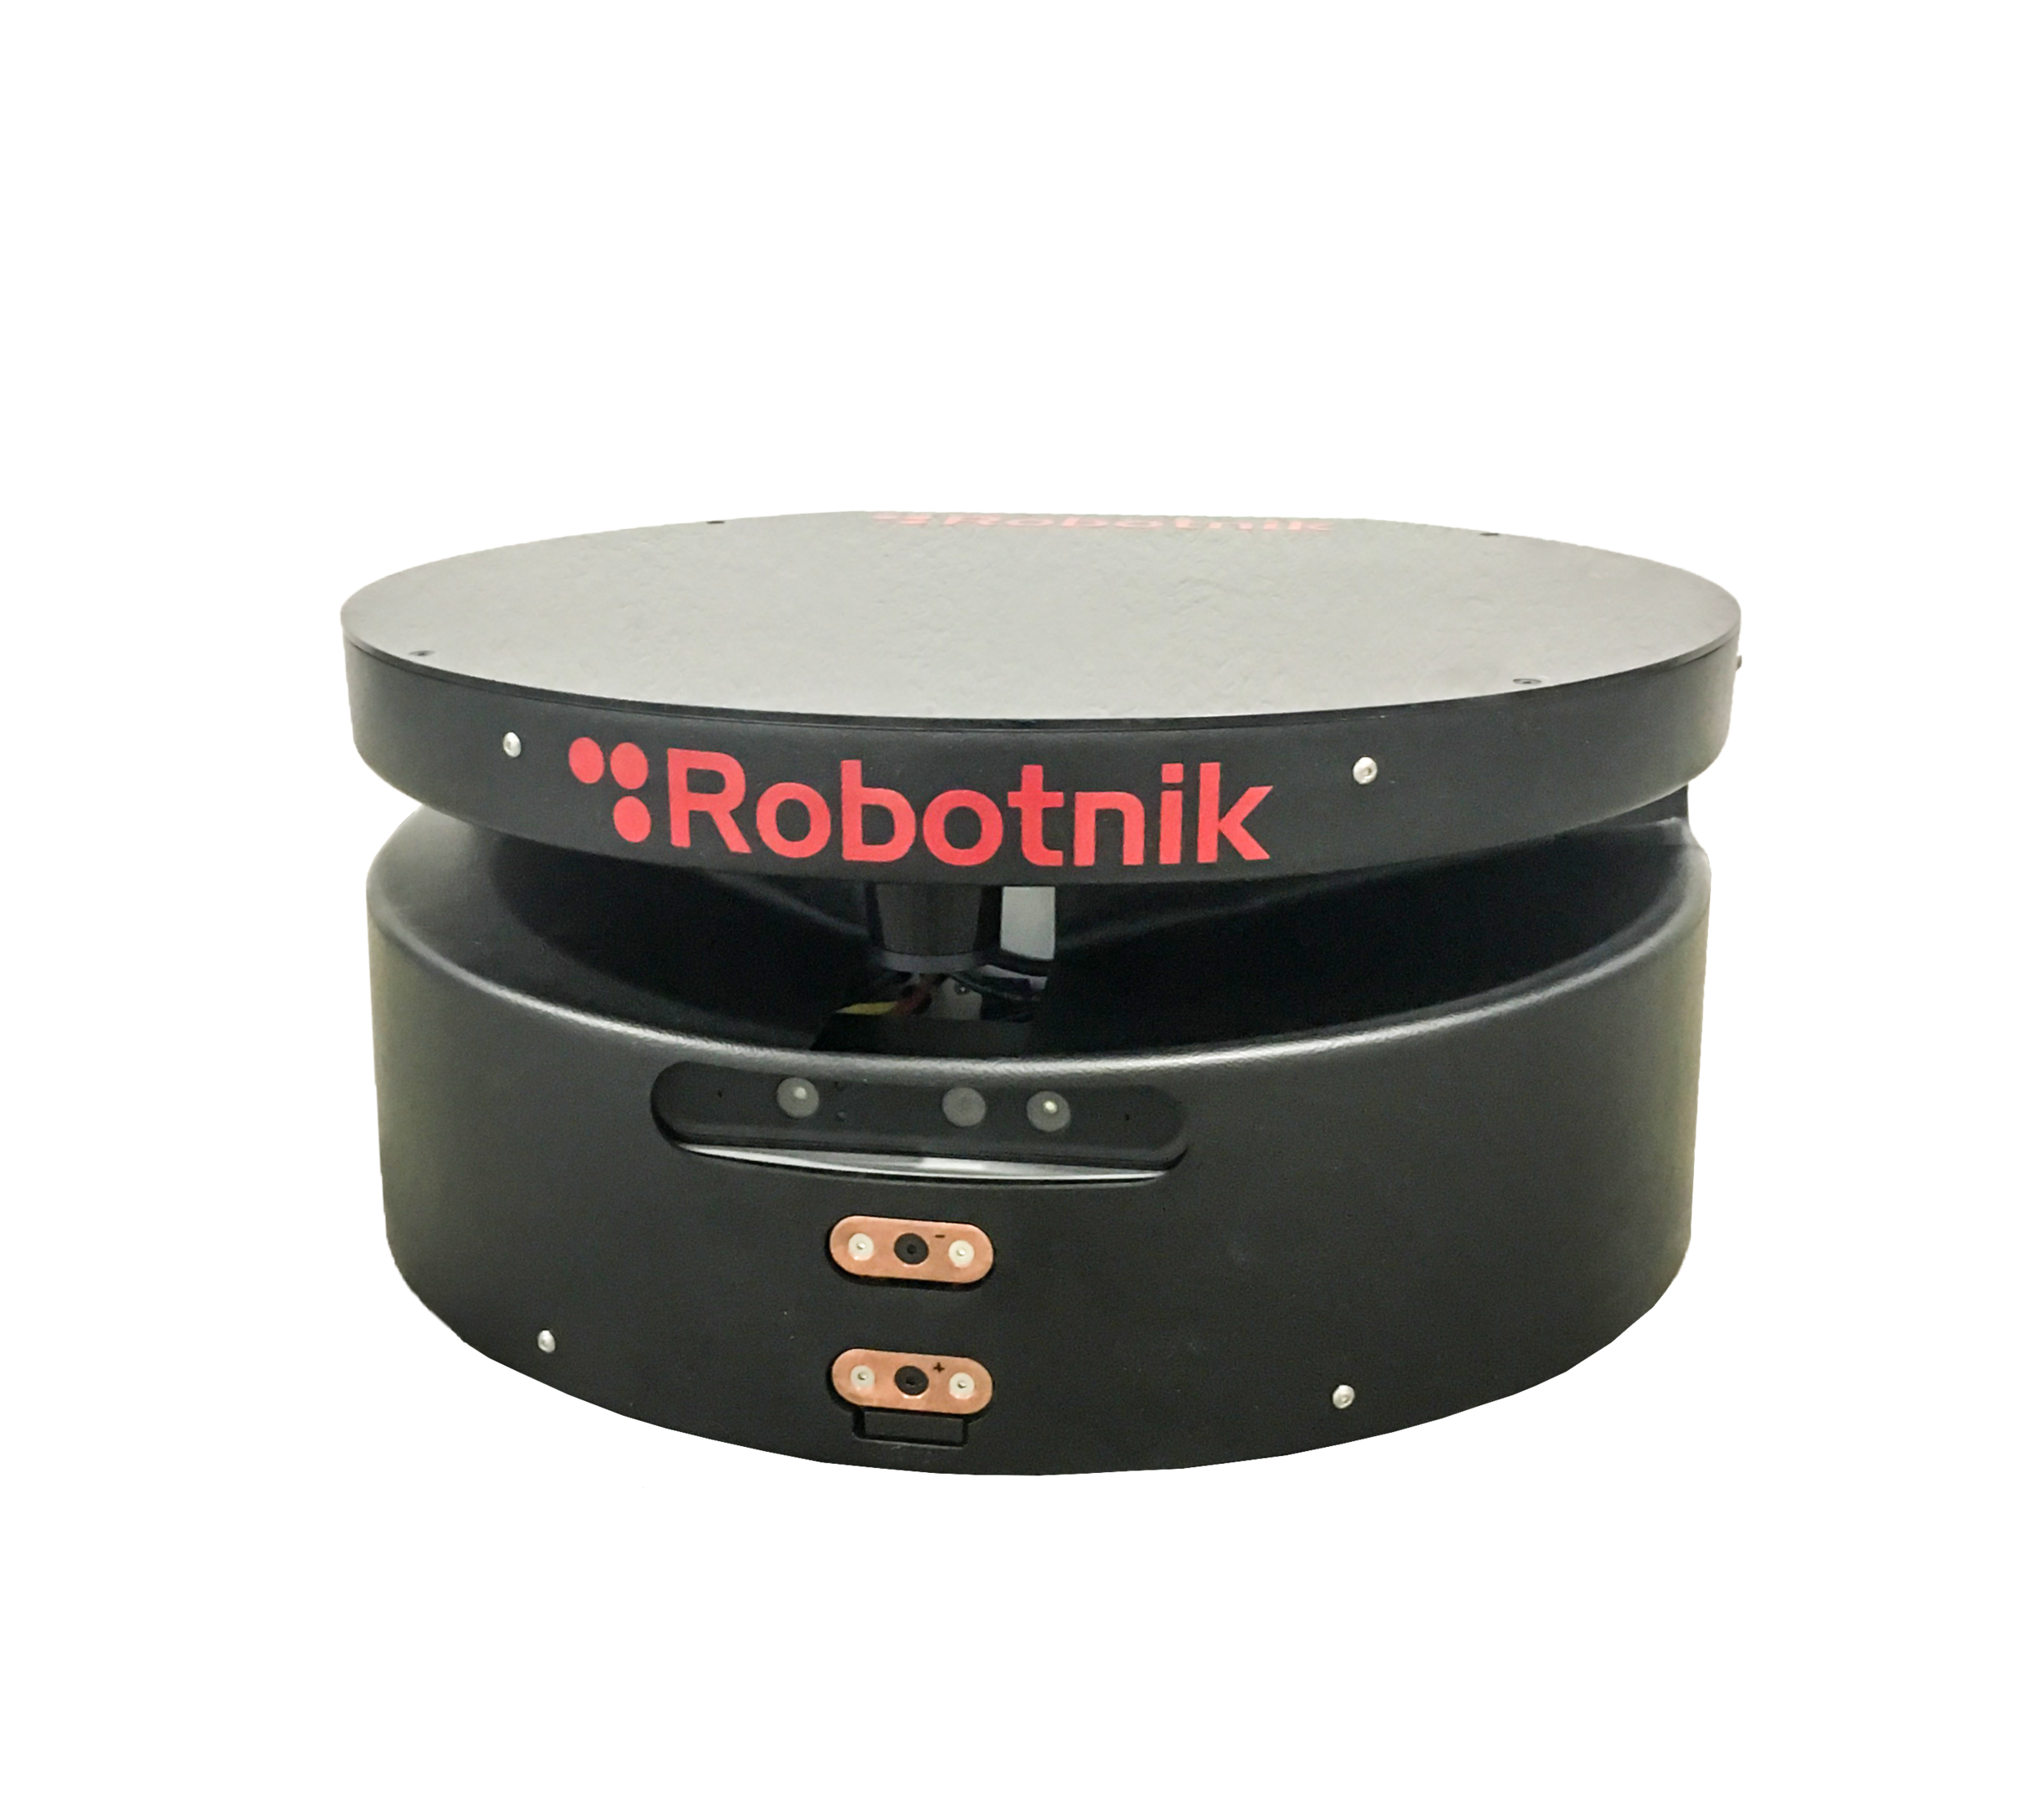
\includegraphics[width=\linewidth]{figures/Robotnik_RB-1-BASE-frontal.png}
        \caption{RB-1 BASE}
        \label{fig:rb1_base}
    \end{subfigure}
    \begin{subfigure}[b]{0.25\linewidth}
        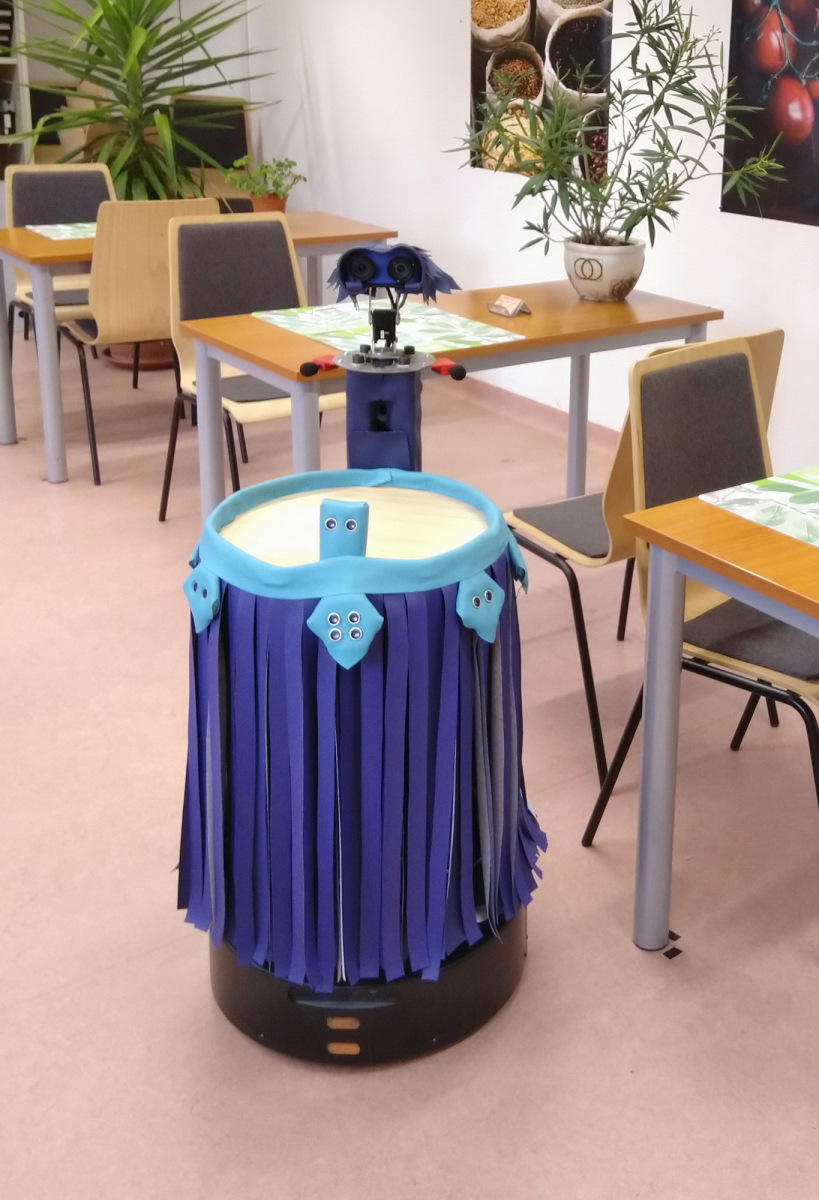
\includegraphics[width=\linewidth]{figures/biscee_frontal.jpg}
    \caption{biscee}
    \label{fig:biscee}
    \end{subfigure}
    \caption{Példák non-humanoid robotokra filmekben.}
    \label{fig:base_and_biscee}
\end{figure}
Erre bővítésképp egy felépítmény készült, melyen a kiszállítandó ételek elhelyezhetőek. A robot jelenleg ezek mozgatására alkalmas manipulátorral nem rendelkezik, a személyzetnek és a vendégeknek maguknak kell elhelyezni és elvenni a kívánt dolgokat. Az alap szenzorkészlet kiegészítésre került továbbá 8, navigációra és kommunikációra szolgáló ultrahang szenzorral és egy mozgatható fejrészen kialakított kamerára. Mivel az ember számára a szem páros szervként hat természetesen valójában két kamera is elhelyezésre került egymás mellett, azonban ebből jelenleg praktikus okokból csupán egy üzemel. Manapság jellemzően valamilyen polimer borítást alkalmaznak hasonló célú kísérleti robotoknál, ez azonban meglehetősen steril kinézetet okozhat. Biscee ehelyett műbőr borítást kapott, mely lényegesen kevésbé kelt mesterséges hatást. A megoldás emellett költséghatékony és a fejlesztés során rugalmasan alakítható és könnyű hozzáférést biztosít az alkatrészekhez és a kábelezéshez. A fent leírtak megfigyelhetőek a \ref{fig:biscee}.ábrán.

A munka során első lépésben másodlagos feladatként a bázisrobot szimulációját kiegészítettem a felépítmény extra szenzoraival és ROS nodejaival. A szimuláció futtatható mind virtuális környezetben mind konténerizálva, ily módon előzetes, biztonságos tesztelési lehetőséget biztosítva a robot mozgását és viselkedését fejlesztő munkatársaim számára. Elsődleges feladatom a roboton található kezdetleges arcfelismerő megoldás továbbfejlesztése volt. Ennek potenciális felhasználási lehetőségei sokrétűek, elsődleges kitűzött célja az előző gondolkodási vonalat követve a következő.

A kitűzött célfeladat alapvető szociális interakciót, kommunikációt igényel. Amennyiben ez nincs jelen a biztosított megoldás a magasan specializált, drága infrastruktúra kiváltásán túl nem nyújt lényegi előnyt például a futószalagos kiszolgálással szemben. Mindennapi életből származó intuitív tapasztalataink alapján kijelenthető, hogy kellemetlen, mikor egy vendéglátásra szakosodott létesítménybe betérve nem érezzük a kiszolgáló személyzet felénk irányuló figyelmét. Természetesen a túlságosan intruzív figyelem is negatív érzelmeket kelthet, azonban későbbi viselkedésbeli mintatervezési feladat. Fontos tehát, hogy a felszolgálási feladat előzetes lépéseként képesek legyünk kifejezni a vendég számára a felé irányuló figyelmet.

Az emberi kommunikáció egyik igen fontos nonverbális összetevője a szemkontaktus. Alkalmazása azonban nem korlátozódik ember-ember kapcsolatokra. Fő érzékszervként az állatvilágban is lényeges szerepet játszik, így kisállatainkkal folytatott interakcióink során is előszeretettel használjuk. Kutyáknál például az emberekhez hasonlóan megfigyelhető a szemlesütés és hasonló viselkedések, de helyzettől függetlenül is szeretünk állatokhoz tekintet és kinézet alapján hangulati tartalmat kapcsolni. A szemek emellett a verbális kommunikációt nem vagy csak korlátozottan alkalmazó képzeletbeli karakterek érzelemkifejezésében is fontos szerepet játszanak ezzel bizonyítva, hogy fontosságuk a való világ keretein is túlnyúlik. Ezekre látható néhány példa a
\todo{ábra}
.ábrán.
\begin{figure}
    \centering
    \begin{subfigure}[b]{0.24\linewidth}
        
\includegraphics[width=\linewidth]{figures/eye/grumpy_cat.jpg}
    \end{subfigure}
    \begin{subfigure}[b]{0.24\linewidth}
        
\includegraphics[width=\linewidth]{figures/eye/doge.jpg}
    \end{subfigure}
    \begin{subfigure}[b]{0.24\linewidth}
        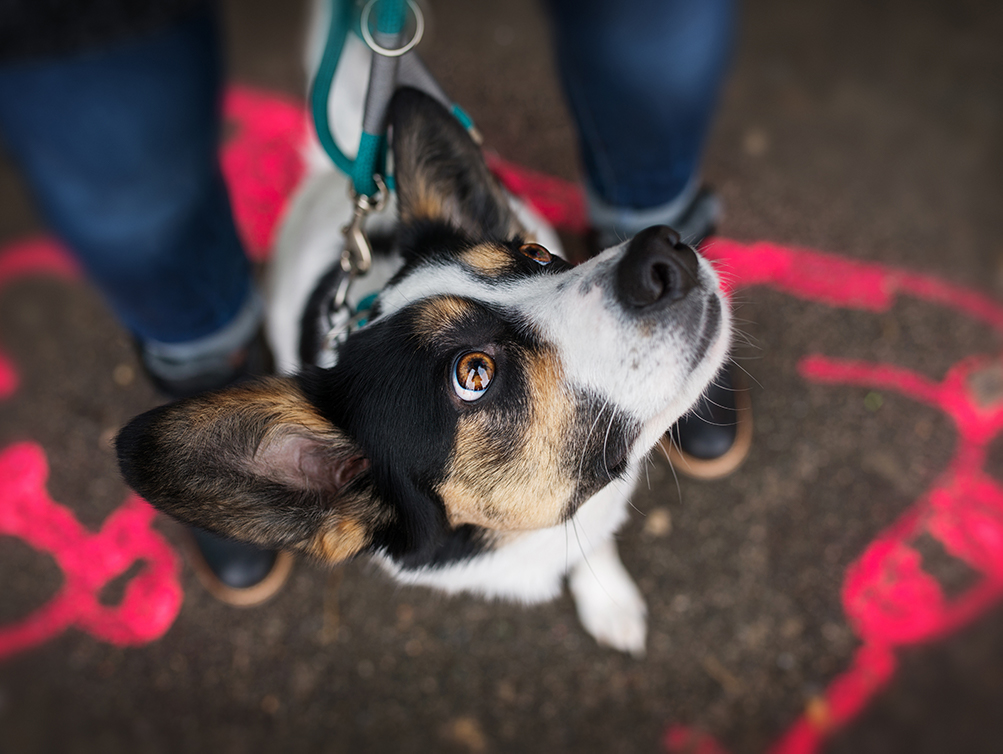
\includegraphics[width=\linewidth]{figures/eye/dog_attention.jpg}
    \end{subfigure}
    \begin{subfigure}[b]{0.24\linewidth}
        
\includegraphics[width=\linewidth]{figures/eye/wp1816244.jpg}
    \end{subfigure}
    \caption{Példák non-humanoid robotokra filmekben.}
    \label{fig:eye_importance}
\end{figure}
A tekintet az adott személy felé irányítása, a szemkontaktus felvétele a kommunikációs csatorna megnyitásának szempontjából kulcsfontosságú nonverbális eszköz. Az első szempontjából elégséges, a második szempontjából pedig szükséges ehhez az alany arcának helyzetének ismerete. Ennél fogva szükségessé válik valamilyen szintű arcfelismerési módszer alkalmazása. Ennek szintjét és módját, az alkalmazott szenzorokat és algoritmusokat az adott helyzethez és limitációkhoz kell igazítani. Esetünkben a szenzorok és a hardver adottak: Biscee kamerái és az RB1-es platform hardvere. Adottak továbbá a roboton futó jelenlegi Ubuntu Linux operációs rendszer és ROS verzió. A roboton előzetesen futó kezdetleges megoldás a feladatot számosítás nélkül aránylag megfelelő pontossággal és 2 fps sebességgel képes ellátni. A cél ennek lehetőségekhez mért javítása volt.

Mivel a fejlesztőgárdában kapcsolódó területeken tapasztalt személy nem szerepelt, első lépésben a témában fontos alapvető fogalmak, illetve a jelenleg elterjedt megoldások gyakorlati és rövid elméleti megismerésével kezdtem. Ezt követően részletesebb irodalmi kutatást végeztem a létező arc- és objektumfelismerő eljárásokról és az ezeknél alkalmazott benchmark teljesítményértékelési lehetőségekkel kapcsolatban. Következő lépésben a létező algoritmusok körét leszűkítettem a célfeladatnak és hardveres limitációknak megfelelően, majd ezeket kiértékelve összehasonlítottam. A kiválasztott algoritmust a roboton futó ROS rendszerrel kompatibilis nodeban helyeztem el. A kutatás menetét és a kapott eredményeket a következő fejezetekben tárgyalom.
\todo{ide még lehetne írni pár mondatot az erőforrások optimalizálásáról (gnome kilövés, túlpörgő websocket node)}      % Bevezetés
\chapter{Háttér}
Az emberi arcfelismerés elfogadott modelljég Burce és Young \cite{bruce_understanding_1986} dolgozták ki 1986-ban. A \ref{Bruce_and_Young_face_recognition_model}. ábrán vázolt modellen jól látható, hogy a probléma igen összetett, több alfeladatra osztható, melyek egyenként további lépésekre bonthatóak szét. Első lépésben az érzékelt kép alapján egy első lépés minden esetben az arc strukturális kódolása, mely alapján a különböző felismerési és hozzárendelési feladatok elvégezhetőek.

\begin{figure}
    \centering
    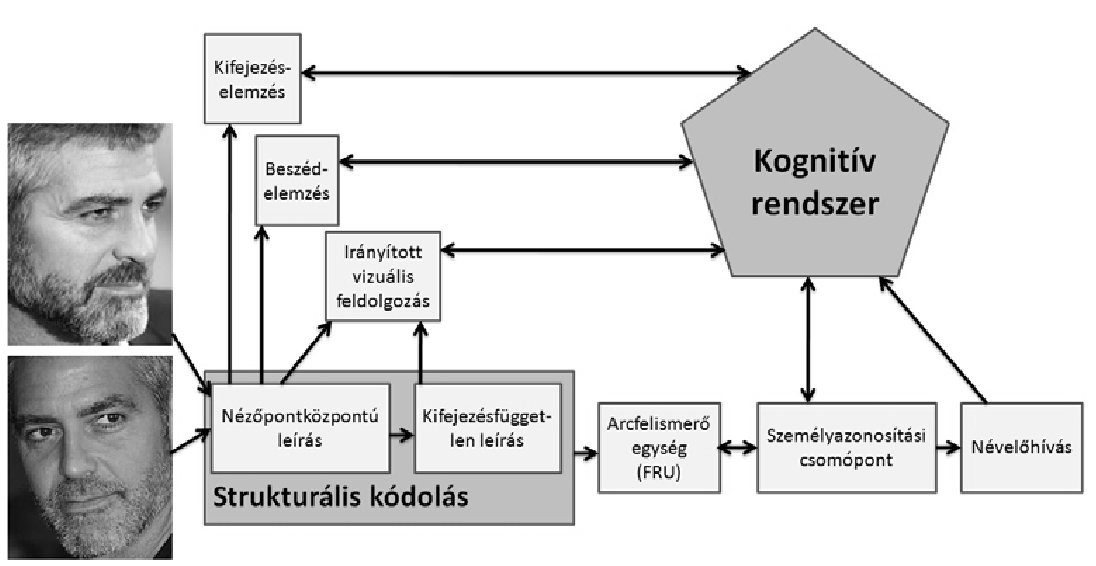
\includegraphics[width=\linewidth]{figures/bruce-young.png}
    \caption{Bruce és Young arcfelismerési modellje. \cite{kornel_az_2015}-ból átemelve.}
    \label{Bruce_and_Young_face_recognition_model}
\end{figure}

Amennyiben ezt számítógépen kívánjuk megvalósítani első lépésben szükségessé válik az adott képen található arcok képen belüli helyzetének meghatározása melyet arcdetekciónak nevezünk. Ezt hozzávéve a modellünkhöz megkapjuk a gépi arcfelismerésben alkalmazott felosztást: arcdetekció, jellemzők kinyerése, majd ezek alapján a felismerés (személyazonosítás, hangulatfelismerés, etc.).

A robot kialakítását, az elvégzendő feladatot és a hardver limitációit tekintve ezen feladatok közül csupán az elsőt, a detekciót kívánjuk elvégezni. A feladatok párhuzamosíthatóságának köszönhetően amennyiben szükségessé válnak és az erőforrások engedik további nodeok hozhatóak létre ezek elvégzésére.

\section{Arcdetekció}

\subsection{Definíció}
"Az arcdetekció célja egy adott tetszőleges képen annak meghatározása, hogy a képen találhatóak-e arcok és amennyiben igen ezek pozíciójának és méretének megadása." \cite{yang_wider_2016} \todo{ide jöhetne az a cikk is, amit a wideresek hivatkoznak}

Ez a gyakorlatban majdnem minden esetben az arcot tartalmazó négyzet alakú terület, ún. bounding box meghatározását jelenti.

\subsection{Irodalmi áttekintés}
Lévén az arcdetekció elsődleges feltétel a különböző arcelemző eljárásokhoz és emellett a vizuális ember-gép és ember-robot interakció alapja lehet, a terület régóta kutattott. Korai munkákat találhatunk akár több mint 50 évvel korábbról is \cite{chan_man-machine_1965,sakai_computer_1972}. A '90-es években számos más kutatási területhez hasonlóan itt is robbanásszerű fejlődés volt tapasztalható \cite{yang_detecting_2002}.

\subsubsection*{Pre-deep-learning korszak}

\paragraph{Viola \& Jones}\hfill

Az első valódi praktikus megoldást azonban Viola és Jones \cite{viola_robust_2004} munkája hozta el. A módszer három kiemelkedő ötletet alkalmazott a valós idejű futás elérésének érdekében: az integrál képet, a figyelem-kaszkádot és az AdaBoost tanulóalgoritmust.

Integrál kép: 
A summed-area table (összesített terület táblázat) használatának ötletét 1984-ben Frank Crow vezette be a számítógépes grafika területén \cite{crow_summed-area_1984} mipmapokban történő alkalmazásra. Az integrál kép elnevezés Viola és Jones munkája folytán vált a módszer elterjedt alternatív elnevezésévé. Az algoritmus a Haar-szerű funkciók gyors számításához használja. Az eredeti képből a következőképpen számolható:
\begin{equation}
    ii(x, y) = \sum_{x' \leq x, y' \leq y} i(x', y'),
\end{equation}
ahol $ii(x, y)$ az integrál kép egy adott $(x, y)$ képpontban, $i(x', y')$ pedig az eredeti kép pixelei. Ebből a képpontok összege a kép bármely ABCD pontok által meghatározott négyszögletű területén (lásd \ref{fig:integral_image_and_haar-like_features}) a következőképp számolható:
\begin{equation}
    \sum_{(x, y) \in ABCD} i(x, y) = ii(D) + ii(A) - ii(B) - ii(C)
\end{equation}
Mivel a Haar-szerű funkciók 2-4 súlyozott négyszögletes területek összegeképp képezhetőek (lásd \ref{fig:integral_image_and_haar-like_features}. ábra) és egy-egy terület kiszámításához így csupán négy darab tömb referencia szükséges a számítás költsége jóval alacsonyabb lesz.

AdaBoost tanulás:
A boostolás névre hallgató metódusok lényege, hogy sok gyenge, közepes pontosságú hipotézis kombinációjaként igyekeznek találni egy magas pontosságú hipotézist. Az eredeti AdaBoost (Adaptive Boosting) \cite{freund_decision-theoretic_1997} algoritmus megnyitotta az utat a későbbi praktikusabb boosting eljárások felé \cite{freund_decision-theoretic_1997}. A diplomamunkának nem célja a boosting eljárások részletesebb ismertetése, amennyiben az olvasó betekintést kíván nyerni a területre Meir és R{\"a}tsc cikke \cite{meir_introduction_2003} jó kezdőpontot szolgáltat.

\begin{figure}
    \centering
    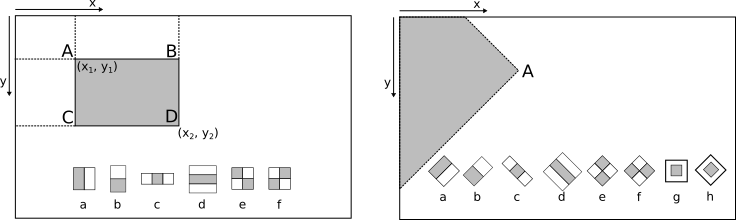
\includegraphics[width=\linewidth]{figures/integral_img_and_haar.png}
    \caption{Bal oldal: Összesített terület táblázat / integrál kép és Haar-szerű funkciók (a-f). Jobb oldal: Példa a későbbi lehetséges kiegészítésekre. Elforgatott integrál kép és két újabb Haar-szerű funkció (g, h).}
    \label{fig:integral_image_and_haar-like_features}
\end{figure}

Figyelmi kaszkád:
A figyelmi kaszkád az integrál képen túl az algoritmus másik sebesség szempontjából kritikus eleme. A megfigyelés lényege, hogy létrehozhatunk olyan gyengébb osztályozókat, melyek a negatív ablakok többségét elutasítják, míg a pozitív ablakokat majdnem mind detektálják. Ennek köszönhetően az összetettebb, nagyobb számításigényű osztályozókat már csak jóval kevesebb részletre kell futtatnunk a benn maradt hamis pozitívok kiszűrésére. Ennek sematikus ábrázolása látható a \ref{fig:attentional_cascade}. ábrán.

\begin{figure}
    \centering
    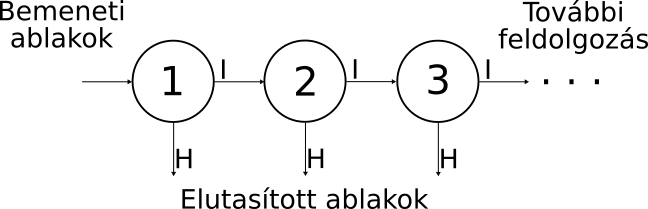
\includegraphics[width=\linewidth]{figures/attentional_cascade.png}
    \caption{Figyelmi kaszkád}
    \label{fig:attentional_cascade}
\end{figure}

Az eredeti cikkben \cite{viola_robust_2004} a figyelmi kaszkádot kézzel állították össze. Ez azt jelenti, hogy az osztályzók számát és elutasítási küszöbét manuálisan kellett specifikálni. Ez igen nehéz feladat, hiszen amennyiben túl szigorúan állítjuk össze a feltételeket gyors, ám gyenge detekciós rátájú detektort kapunk. Amennyiben az ellenkező irányba térünk ki a detektor ugyan pontos lesz, ám lassú is.

A módszer továbbfejlesztésére nagy mértékű kísérlet irányult. Ezek többnyire a következő módosításokkal álltak elő:

\begin{itemize}
    \item A téglalap alakú jellemzők lecserélése vagy kibővítése valamilyen módon, például az eredeti jellemzők 45 fokos elforgatásával \cite{lienhart_extended_2002}.
    \item Különböző új, optimálisabb tanítási eljárások alkalmazásával.
    \item Különböző formában elrendezett figyelmi kaszkádok alkalmazása (\ref{fig:alternative_attentional_cascades}).
\end{itemize}

\begin{figure}[h]
    \centering
    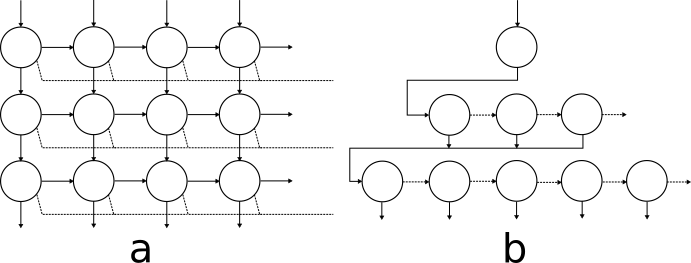
\includegraphics[width=\linewidth]{figures/alternative_cascades.png}
    \caption{Alternatív figyelmi kaszkád struktúrák. A szaggatott nyilak az elutasítást, míg a folytonosak az elfogadást jelzik. a: parallel kaszkád\cite{bo_wu_fast_2004} b: detektor-piramis \cite{goos_statistical_2002}}
    \label{fig:alternative_attentional_cascades}
\end{figure}
\todo{ehhez az ábrához még tudnék szedni alternatívákat és hivatkozásokat}
\todo{egybevonni a sima figyelmi kaszkád ábrát és ezt}

\paragraph{Konvolúció a képfeldolgozásban}\hfill

A képfeldolgozás egyik legfontosabb eszköze a képtérbeli konvolúciós művelet. A módszer lényege, hogy egy konvolúciós ablaknak nevezett mátrix segítségével súlyozva összegezzük a pixelünket a környezetével. Középpontos ablakot feltételezve ez képpontonként a következő módon számítható:
\begin{equation}
    G(i,j) = (I * K)_{ij} = \sum_{u = -m}^{m} \sum_{b = -n}^{n} I(u, v) K(i - u, j - v)
\end{equation},
ahol
\begin{itemize}
    \item \(G(i,j)\) a konvolúció eredménye az \((i, j)\) pontban
    \item \(I(i, j)\) a kép \((i, j)\) pixelének értéke
    \item \(K(i, j)\) a konvolúciós ablak \((i, j)\)-ik értéke
    \item \(m\) a konvolúciós ablak szélességének fele lefelé kerekítve
    \item \(n\) a konvolúciós ablak szélességének fele lefelé kerekítve
\end{itemize}

\begin{figure}[h]
    \centering
    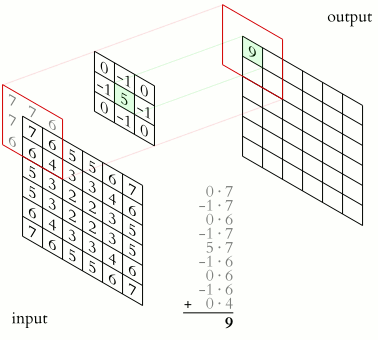
\includegraphics[width=0.5\linewidth]{figures/2D_Convolution.png}
    \caption{Konvolúció képeken.}
    \label{fig:2d_convolution}
\end{figure}

A művelet elvégzésének vizuális magyarázata sokkal intuitívabb. Tegyük fel, hogy a konvolúciós ablakot az
\ref{fig:2d_convolution}. ábra
szerint a képünk bal felső sarkára helyezzük, majd az egy helyre került értékeket összeszorozzuk és a szorzások eredményét összeadva beírjuk az eredményül kapott képünk bal felső sarkába. Ez után az ablakot egy sorral jobbra helyezve a műveletet megismételjük és az eredményt beírjuk az előzőtől egyel jobbra. Mikor egy adott soron végigérünk ugrunk a következő sor elejére, melynek eredményeit a kimenetünk következő sorába írunk. Az ábrán látható, hogy így az eredetihez képest m+1 pixellel keskenyebb és n+1 pixellel alacsonyabb kimenetet kapunk. Ennek kiküszöbölésére paddinget (tömés, bővítés) szokás alkalmazni, mely lényegében egy valamilyen módon megválasztott kiegészítés, keret a képünk számára. Bizonyos esetekben azonban kívánatos lehet a dimenziócsökkentés, ilyenkor megtehetjük, hogy az ablakot több soronként "ugráltatjuk". Ezt a mértéket stridenak (lépcsőzés) nevezik.

Konvolúcióval számtalan képfeldolgozási feladat végezhető el, például szűrések, simítások és különböző irányú éldetektálás.
\todo{opcionálisan ábra}

\paragraph{Histogram of Oriented Gradients (HoG)}\hfill

Bár az irányított gradiensek módszerének ötlete jóval az ezredforduló előttről származik\cite{william_t_freeman_orientation_1994,mcconnell_method_1986}, népszerűvé Dalal és Triggs\cite{dalal_histograms_2005} gyalogosfelismerő módszerének 2005-ös publikálása után vált. Amennyiben a képre \(f(x, y)\) kétváltozós folyamatos függvényként tekintünk annak gradiens vektorát a következő módon számíthatjuk:
\begin{equation}
    \nabla f = |\overline{\nabla f}| = \sqrt{\left(\frac{\partial f}{\partial x}\right)^2 + \left(\frac{\partial f}{\partial y}\right)^2} \approx \left| \left(\frac{\partial f}{\partial x}\right) + \left(\frac{\partial f}{\partial y}\right) \right|
\end{equation}
Digitális képeken ezt a következőképp közelíthetjük:
\begin{equation}
    \nabla f = 
    \begin{bmatrix}
        \frac{\partial f}{\partial x} \\
        \frac{\partial f}{\partial y}
    \end{bmatrix}
    =
    \begin{bmatrix}
        \delta x \\
        \delta y
    \end{bmatrix}
    \approx
    \begin{bmatrix}
        \Delta x \\
        \Delta y
    \end{bmatrix}
\end{equation}
A vektor irányát pedig a következezőképp kaphatjuk meg:
\begin{equation}
    \alpha (x,y) = \arctan \left(\frac{\delta x}{\delta y}\right)
\end{equation}

Az eredeti cikkben több különböző konvolúciós maszkot is teszteltek ennek számítására különböző mértékű Gauss-simítást követően. A legjobbnak az egyszerű \([-1, 0, 1]\) és transzponáltja bizonyultak. A képünket ezután valamilyen stragégia szerint cellákra osztjuk. A vektorokat átváltjuk polárkoordinátákra és a gradiensek terét szög szerint valahány tárolóra osztjuk. Ez után a tárolókat cellánként hisztogram szerűen feltöltjük, azonban a vektorok száma helyett azoknak hosszát adjuk az adott tárolókhoz. Az eredeti cikkben az ellentétes irányú grádiensek egybevonása, tehát a szögek 0 és 180\textdegree közé korlátozása bizonyult, 9 tárolóval. Mivel ez nem túl nagy szám előfordulhat, hogy egy határon lévő grádiens rossz tárolóba kerülne. Ennek kiküszöbölésére érdemes lehet valamilyen stratégia mentén a szomszédos tárolókhoz is hozzáadni annak súlyozott értékét, vagy fuzzy viselkedést vinni a rendszerbe\cite{salhi_histograms_2013}. Ez után a végső HoG jellemzőnket két lépcsős normalizálás után kapjuk. A két lépcső oka, hogy a hisztogramunkat normalizálnunk kell az azonos tárgyat tartalmazó képek közötti kontrasztkülönbségek kiküszöbölésének érdekében. Más részről az gradiensek mértéke egy területen információtartalmat hordoz. Ezért a cellákat először blokkokra osztjuk a teret konvolúciós viselkedés szerint kicsempézve, majd ezeket normalizáljuk. Az euklideszi norma például jó normának bizonyult erre a célra:
\begin{equation}
    b \leftarrow \frac{b}{\sqrt{\Vert b \Vert^2 + \epsilon}}
\end{equation}
\(\epsilon\)-ra a 0 gradiensű blokkok esetén a 0-val való osztás kiküszöbölése miatt van szükség. Ezt követően a kapott eredményeket összefűzzük a végleges HoG jellemzővektorunkba és újra normalizáljuk. A tapasztalat azt mutatja, hogy ebben a lépésben érdemes még egy kiegészítő lépésként visszavágni a kapott nagyon nagy \(h_n\) grádiens eredményeket, mert azok elnyomnák a többit. Ezt követően újra normalizálnunk kell, tehát a folyamat három lépcsőből áll:
\begin{equation}
    \begin{split}
    h \leftarrow \frac{h}{\sqrt{\Vert h \Vert^2 + \epsilon}}\\
    h_{n} \leftarrow \min (h_{n}, \tau)\\
    h \leftarrow \frac{h}{\sqrt{\Vert h \Vert^2 + \epsilon}}
    \end{split}
\end{equation}

A kapott jellemzőteret ez után tetszőlegesen választott klasszifikátorral osztályozhatjuk.

\subsubsection*{Deep learning korszak}
"Az adat az új olaj" - jelentette ki Steve Humby brit matematikus 2006-ban. Amennyiben a ma uralkodó nagyvállalatok profilját tekintjük kijelenthető, hogy állításávan nem tévedett.

Az ezredforduló után a számítási és tárolókapacitás növekedésével, emellett az internet terjedésének köszönhetően robbanásszerűen gyarapodó rendelkezésre álló adatmennyiségnek köszönhetően számos új számítógépes és információtudományi terület látott napvilágot vagy éppen kapott új erőre. Így van ezzel a gépi tanulás mesterséges neurális hálózatokkal foglalkozó területe is. Míg az ezredforduló környékén a Gabor filterek és Support Vector Machineok (SVM) voltak népszerűek és a mai napig használt módszerek, az utóbbi évtizedben a különböző mesterséges neurális hálózatokkal foglalkozó publikációk száma exponenciális növekedésnek indult. Ez jól megfigyelhető a Dimensions\cite{noauthor_dimensions_nodate} \ref{fig:neural_network_article_numbers}. ábrán látható adatain is.

\begin{figure}
    \centering
    \begin{subfigure}[b]{0.45\linewidth}
        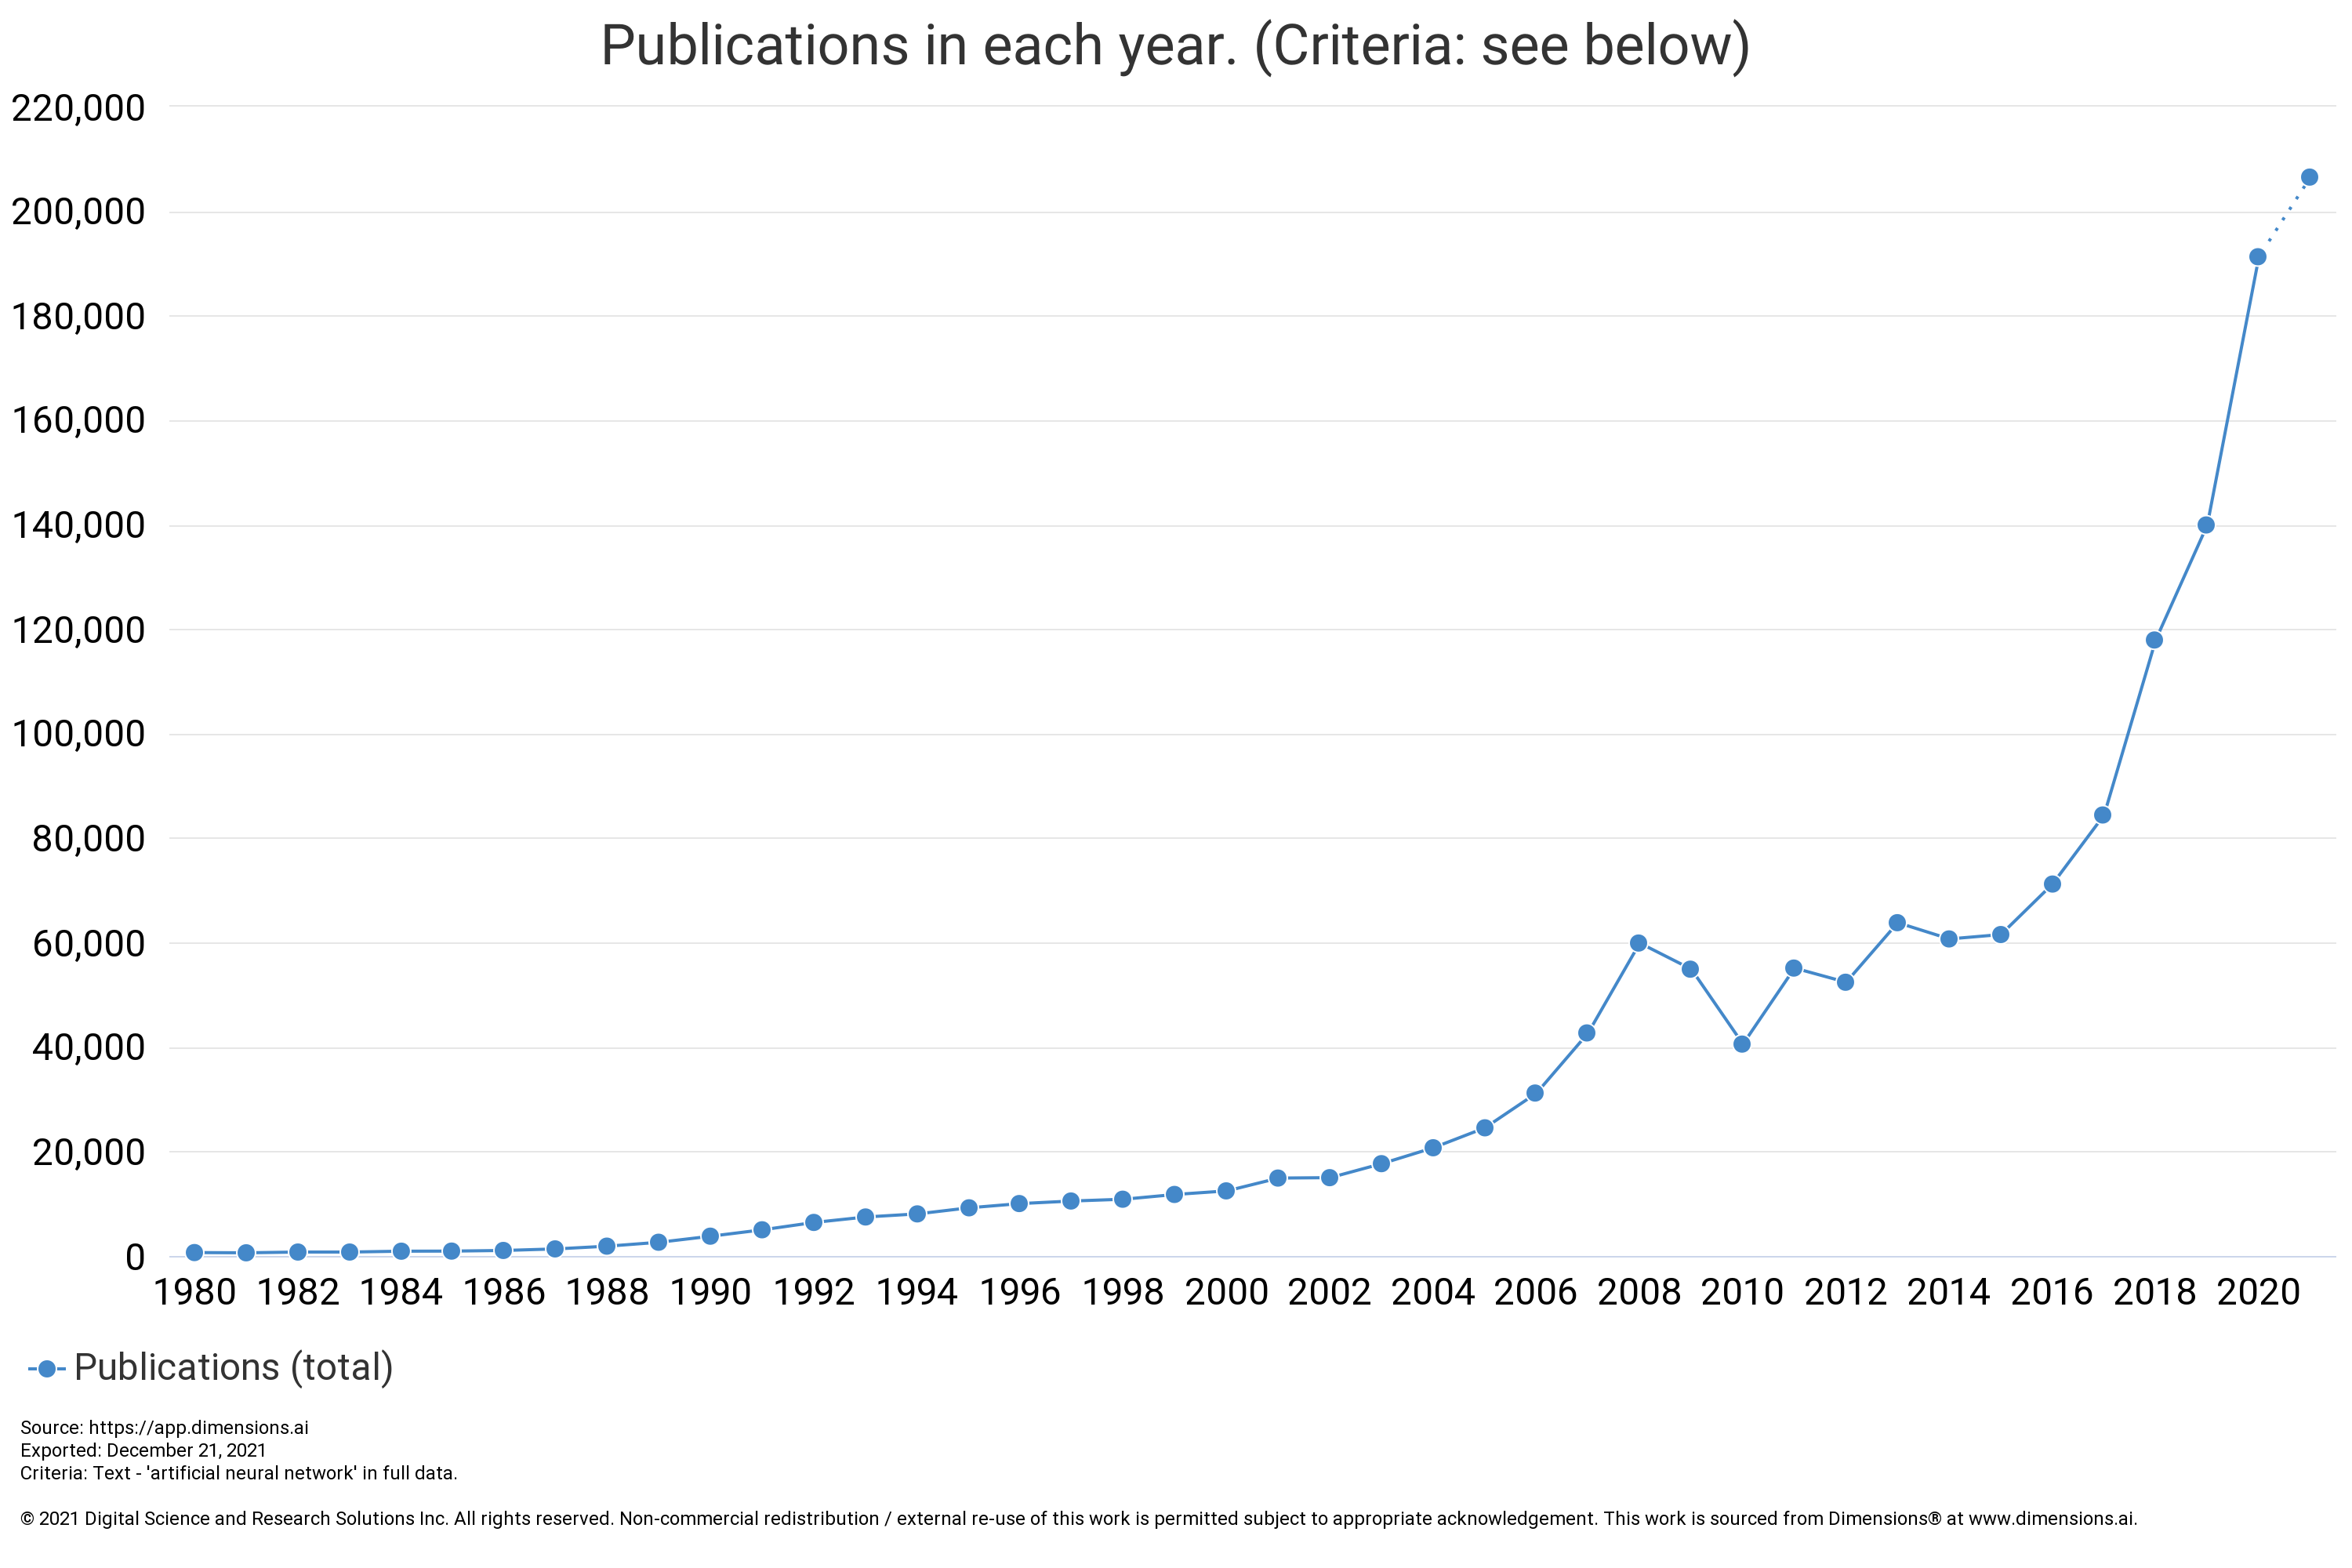
\includegraphics[width=\linewidth]{figures/dimensions_ai_artificial_neural_network_publications.png}
        \caption{Publikációk száma}
    \end{subfigure}
    \begin{subfigure}[b]{0.45\linewidth}
        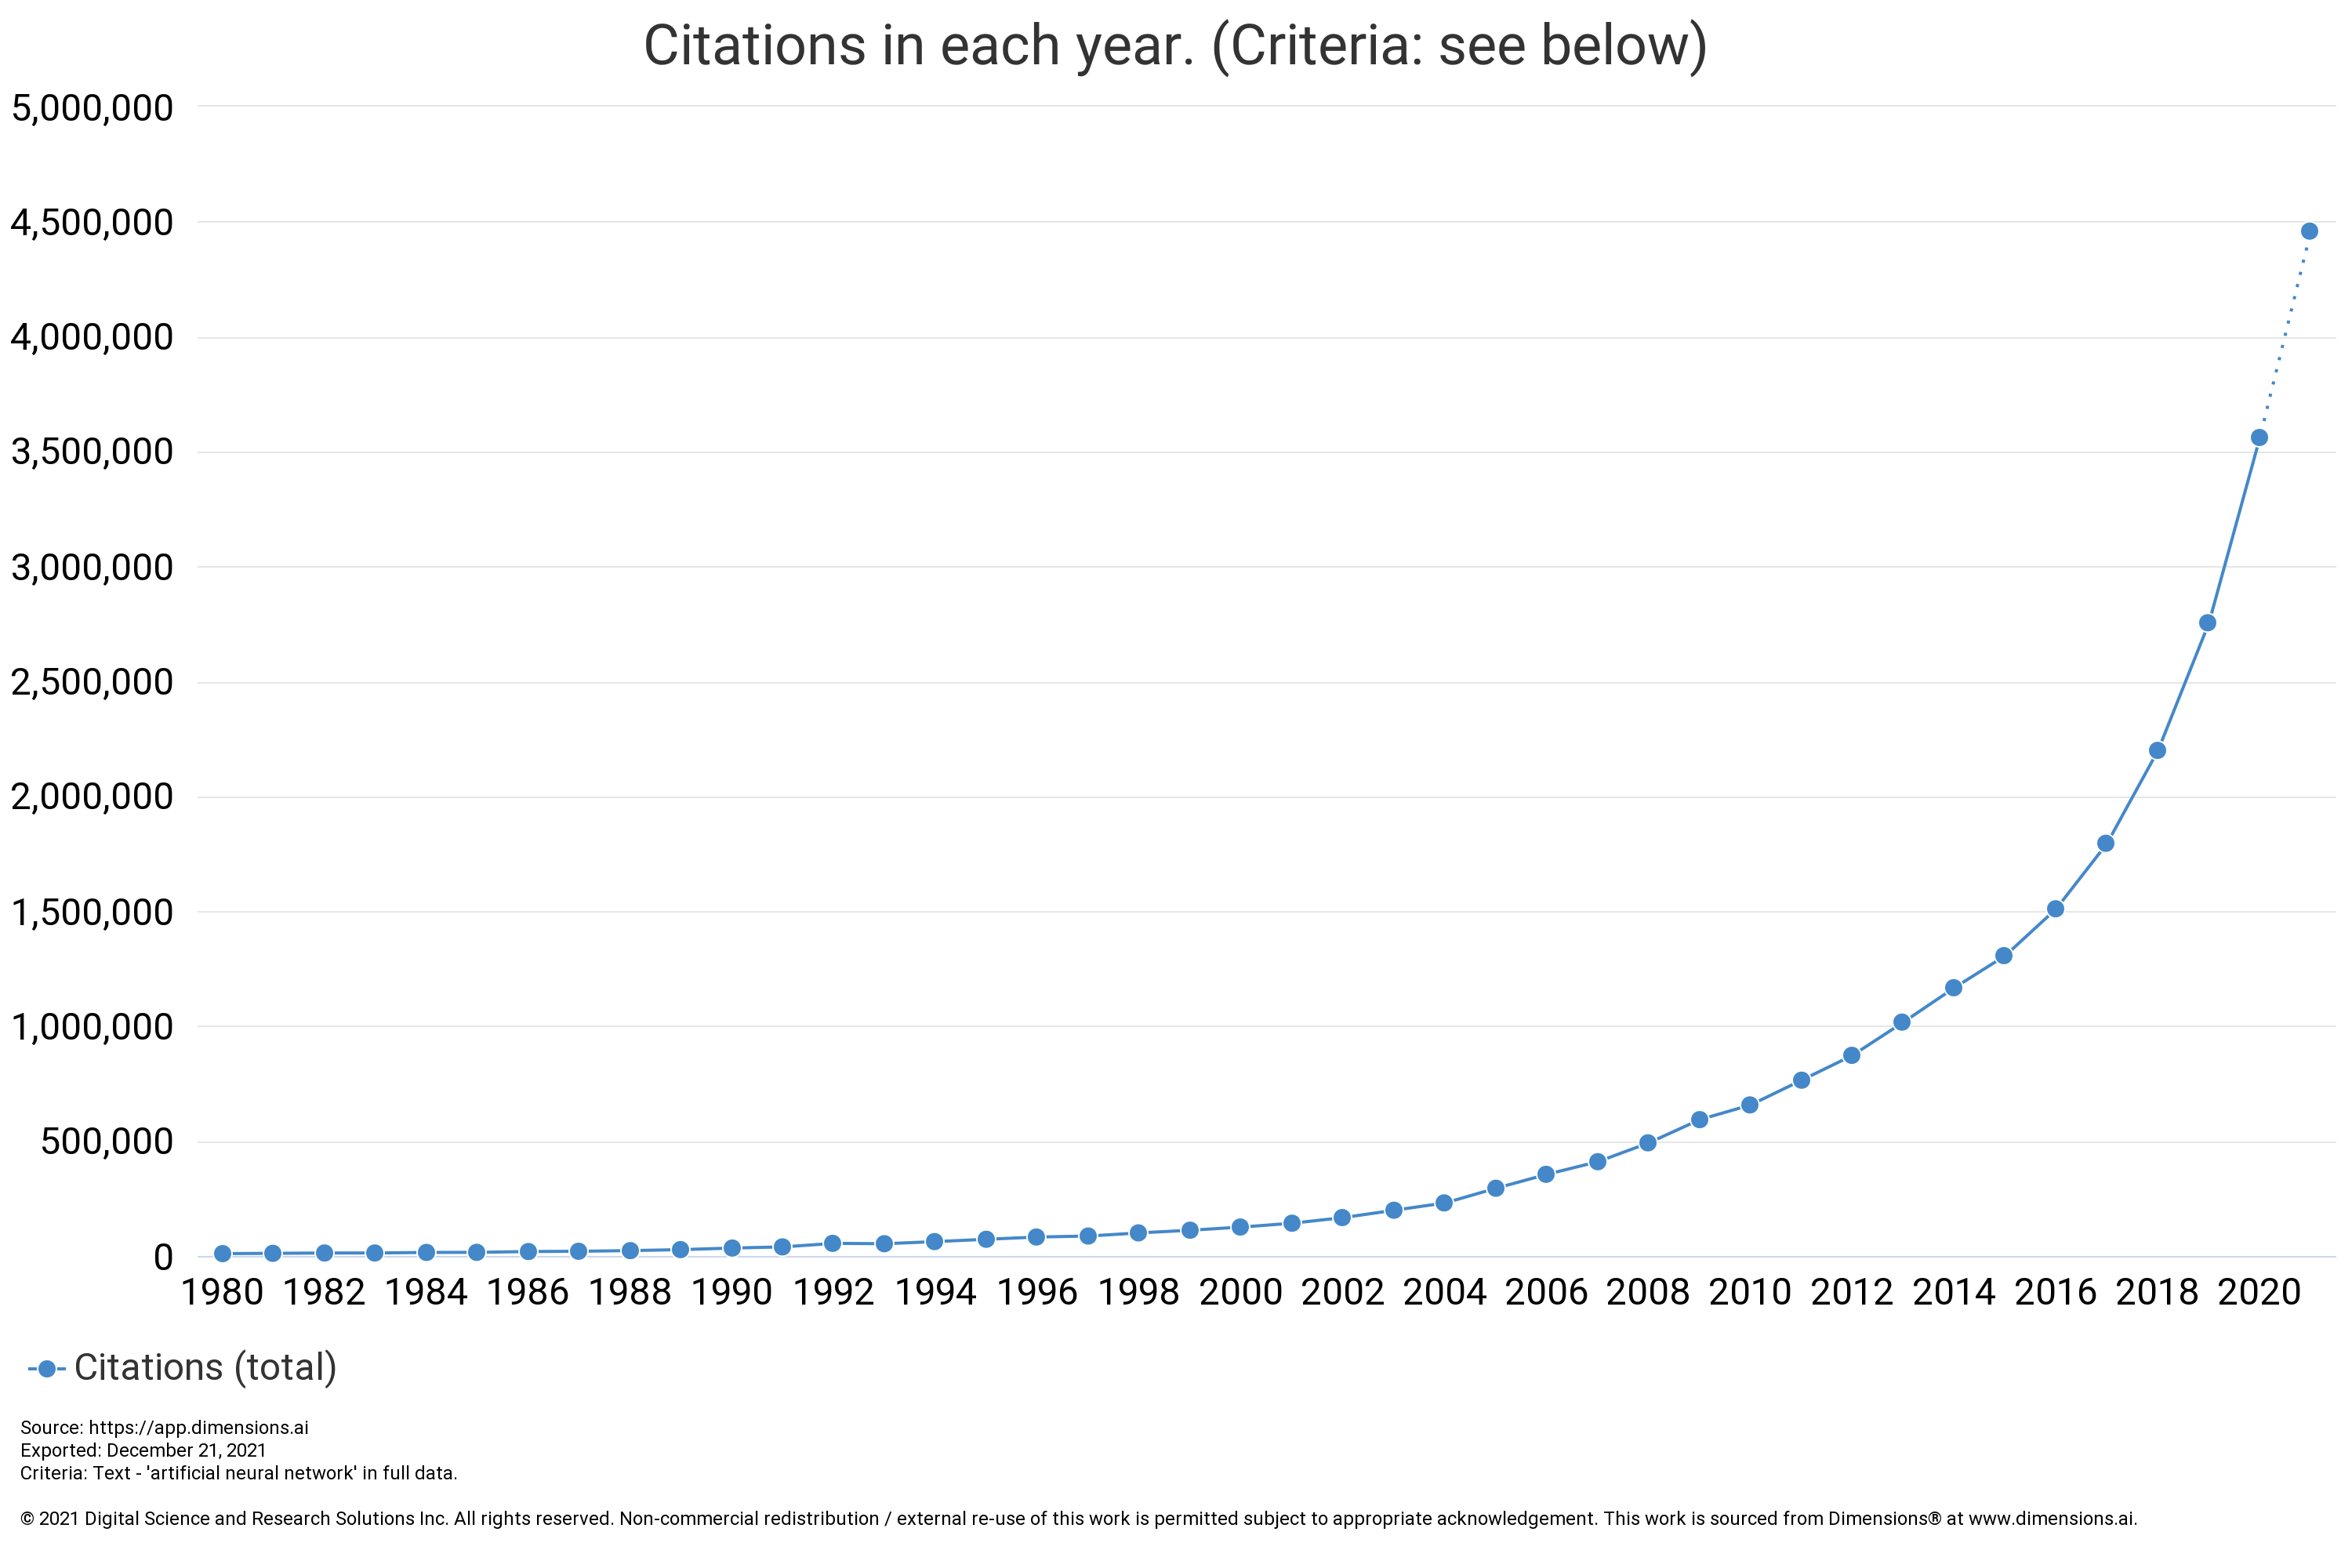
\includegraphics[width=\linewidth]{figures/dimensions_ai_artificial_neural_network_citations.png}
        \caption{Hivatkozások száma}
    \end{subfigure}
    \caption{Mesterséges neurális hálózatokkal foglalkozó publikációk és hivatkozások száma évekre lebontva.}
    \label{fig:neural_network_article_numbers}
\end{figure}

Ez három fő összetevőnek köszönhető. Az első, hogy a felügyelt tanulási módszer magasszintű adatszükséglete egyre több területen biztosított. A második, hogy a számító egységek és a memória növekedésével egyre gyorsabban és egyre nagyobb hálókat tudunk betanítani. Harmadik pedig az ezek hatására elindult kutatások folyamán megalkotott gyorsabb és pontosabb algoritmusok és könyvtárak nem csak jobb eredményeket tesznek lehetővé, de gyorsabb iterációs sebességet is biztosítanak a fejlesztés során.
\todo{ide még lehetne írni arról, hogy az MI és a deep learning diszruptív technológia}

\todo{ehelyett a bekezdés helyett valami értelmeset írni...}
A mesterséges neurális hálózatok és tanításuk részletes ismertetése messze meghaladja ezen diplomamunka kereteit. Amennyiben az olvasó bevezetést kíván nyerni a területre a Deeplearning.Ai\cite{noauthor_deeplearningai_nodate} kurzusai jó kezdőpontot nyújthatnak. Még ha a témát az objektum- vagy akár az arcdetekció témakörére is csökkentjük, a rendelkezésre álló anyagból akár könyvsorozatot is írhatnánk. Ezen okokból most csupán a későbbiekben ismertetett struktúrák megértéséhez minimálisan szükséges eszközkészlet ismertetésére térek ki.

\section{Arcdetekciós benchmarkok}

\subsection{Arcok a vadonban}
Az évek során a különböző arcdetekciós és arcfelismerési eljárások kutatásához és teszteléséhez számos adatszett jelent meg. Azonban a Labeled Faces in the Wild (LFW) megjelenéséig ezeket többnyire jól kontrollált kondíciók között készült képekből állították össze, hogy valamilyen jól specifikált paramétert vizsgálhassanak az arcdetekciós/felismerési területen\cite{huang_labeled_2008}. Ez volt az első megoldás, melynek direkt kitűzött célja a szabad környezetben történő arcfelismerési probléma vizsgálatára szolgáló adatszett nyújtása volt. Ennek köszönhetően az ilyen felállásra legtöbbször az "arcok a vadonban" koncepcióként referálnak. Mára ilyen típusú adatszettek közül kerülnek ki a legnépszerűbbek mind tanítási, mind kiérékelési célokra.

\todo{ide kell kép?}

\subsection{A detekció kiértékelése}
\todo{kell ez? lényegében az IoU-t tudnám leírni ide}

\subsection{FDDB}
2010-ben, az "FDDB: A Benchmark for Face Detection in Unconstrained Settings" \cite{jain_fddb_2010} cikkel nyilvánosságra hozott adatbázis. 2845 képből áll, összesen 5171 felcímkézett arcot tartalmaz. Létrehozásának célja a korábbi létező adatszettek problémáinak kiküszöbölése és protokoll bizosítása az arcdetekciós megoldások összehasonlítására. Alapját a Berg és munkatársai által a Yahoo news 
\todo{Az oldalt ilyenkor be kell hivatkozni?} 
híroldalról származó videókból összeállított adatbázis képzi. Mivel az eredeti sok közel azonos képet tartalmazott első lépésben ezeket 103 csoportba klaszterezték 
\todo{ez amúgy valid szó?}, 
majd mindegyik csoporból egy képet tartottak meg. Ezt követően minden arcot előzetesen felcímkéztek, melynek mérete meghaladta a 20 pixelt. Az alacsony felbontásból, megvilágításból és pozícióból adódó bizonytalanságok kiszűrésére ezután minden képet több emberrel felcímkéztettek egy webes felületen keresztül. Ezen lépésig a szerzők bounding boxokat (dobozokat / négyzet alakú jelölőket) alkalmaztak. A megmaradt arcok dobozait ezek után ellipszisekre cserélték le, mert úgy vélték ez jobb reprezentációja az arcoknak.

\subsection{AFW}
A “Face Detection, Pose Estimation and Landmark Localization in the Wild” \cite{zhu_face_2012} című cikk részeként létrehozott "annotált arcok a vadonban" (annotated faces in-the-wild) adatszett célja a papírban prezentált egyidejű arcdetekciót, pózbecslést és jellemzőkinyerést végző algoritmus kiértékeléséhez egy új, az arcok a vadonban elvet követő megoldást biztosítsanak.

205 Flickr-ről\cite{noauthor_flickr_nodate} származó képet tartalmaz, ezeken összesen 468 annotált arc található. A címkék tartalmazzák az arcot körülvevő dobozt, 6 jellemző pontot és három további, az arc orientációját leíró számot.

A szerzők állítása alapján a képek zsúfolt háttereket és mind megjelenésben, mind pózban változó arcokat tartalmaznak, bár ezek mértéke nincs külön számszerűsítve.

\subsection{PASCAL Face}
A "Face detection by structural models" \cite{yan_face_2014} szerzői az előző két adatszetten túl a Pascal VOC \cite{everingham_pascal_2010} objektumdetekciós és kategorizációs kihívás adatainak arcokra történő szűkítésével egy új mércét is alkalmaztak.

851 képet tartalmaz, ezeken 1335 nagyban különböző arc található (bár a különbözőség itt sincs számosítva). A jelölések és a kiértékelési módszer megegyezik a Pascal VOC-al.

\subsection{WIDER FACE}
Az arcdetekció nagy erővel kutatott területén tapasztalható előrelépések jelentős részben a különböző gépi tanulási módszerekben történő előrelépéseknek köszönhetőek. Jelenleg a mélytanulási eljárással tanított neurális hálózatok uralják a területet. Ezek adatigényességéből kiindulva nem meglepő, hogy az előrelépések nagymértékben az elérhető egyre bővebb és részletesebb adatszetteknek köszönhetőek. Ezen a vonalon gondolkodva jött létre a 2016-ban publikált "WIDER FACE: A Face Detection Benchmark" \cite{yang_wider_2016} adatszett. Publikálásakor az akkoriban elérhető egyéb megoldásokhoz képest nagyságrendbeli növekedést jelentett mind a képek száma, mind az annotált arcok száma tekintetében. Emellett az egy ével korábban publikált MALF \cite{bin_yang_fine-grained_2015} adatkészlet után a második olyan megoldás, mely részletesebb címkéket biztosít a részletesebb kiértékeléshez (és tanításhoz) az arcok pozícióját és takarását illetően. A MALF szetthez képest továbbá a képen látható eseményekkel kapcsolatos címkék is rendelkezésre állnak.

Az adatszett a WIDER eseményfelismerő adatkészlet része, amely 60 különböző eseményből áll. Az esemény kategóriákat a "Large-Scale Concept Ontology for Multimedia" (LSCOM) \cite{naphade_large-scale_2006} elveit követve, illetve diákok véleményét figyelembe vége alkották meg. Ezt követően különböző keresőmotorok használatával kategóriánként 1000-3000 képet gyűjtöttek össze.

A WIDER FACE létrehozásához ezután manuálisan eltávolították az arcokat nem tartalmazó képeket és a diverzitás biztosítása érdekében a hasonló képeket egyet-egyet kivéve eltávolították. Az annotáció során a dobozokat úgy állították be, hogy azok tartalmazzák a homlokot, az állat és az orcákat. A homályosság vagy kis méret (10 pixel alatt) miatt nehezen felismerhető arcokat 'ignore' (figyelmen kívül hagy) címkével látták el. Ezen kívül az arcok pozíciója szempontjából 'typical' (tipikus) és 'atypical' (nem tipikus), kitakartságuk szempontjából pedig 'none' - 'partial' - 'heavy' (nincs - részleges - erős) címkéket hoztak létre. A részleges és erős címkék 1-30\%-os és 30\% feletti takarást jelentenek. Ezeken kívül 'expression' (kifejezés), 'illuminaiton' (megvilágítás) és 'blur' (elmosódottság) címkék is rendelkezésre állnak, bár ezeket a cikk nem részletezi. Az eredeti annotátoron kívül minden címkét két további ember ellenőrzött.

A teljes szettet EdgeBox \cite{zitnick_edge_2014} algoritmust alkalmazva a különböző események detekciós rátáját figyelembe véve könnyű, közepes és nehéz részekre osztották szét. Ezen kívül annak érdekében, hogy az adatok tanításra is felhasználhatóak legyenek véletlenszerűen tanító, validációs és teszt részekre osztották 40\% / 10\% / 50\% arányban. Emellett a cikkben említik, hogy az arcok mérete szerint is szeparálhatóak az adatok, általuk ajánlottan 10-50, 50-300 és 300 feletti méretekre, azonban ezt szükség esetén a dobozok magasságát tekintve sajátkezűleg kell elvégezni.

A képek, a tanító és validációs részek címkéi a WIDER FACE hivatalos oldaláról \cite{noauthor_wider_nodate} bárki számára letölthetőek. A teszt szetten történő kiértékeléshez jelenleg az eredményeket a szerzőknek kell elküldeni, az oldal szerint a közeljövőben automatikus kiértékelésre webszerver készül. A 2016-os publikációt figyelembe véve ezen állítás igazságtartalma kétségbe vonható.

Ennek ellenére amennyiben a teljes adatmennyiség felét tekintjük rendelkezésre állónak, akkor is jelentős méret, nehézség és részletességbeli javulást jelent a korábi népszerű benchmarkokhoz képest. Ezen kívül a tanító- és validációs felosztás rendelkezésre állását tekintve nem meglepő, hogy a WIDER FACE az egyik legnépszerűbb napjainkban elérhető adatszett.

\begin{table}[!ht]
    \footnotesize
    \centering
    \renewcommand{\arraystretch}{1.5}
    \begin{tabular} {|l | c | c |l |}
        \hline
        Név & Protokoll & Annotáció részletessége & Kód \\
        \hline \hline
        FDDB & ROC & Alacsony & Python 2.7 kiértékelő kód, konténerben futtatható \\
        \hline
        AFW & PASCAL VOC & Alacsony & Nem hivatalos Python kód \\
        \hline
        PASCAL Face & PASCAL VOC & Alacsony & Nem hivatalos Python kód \\
        \hline
        WIDER Face & PASCAL VOC & Magas & Matlab kód ellenőrzéshez \\
        \hline
    \end{tabular}
    \caption{Arcdetekciós adatszettek összefoglaló táblázata}
    \label{tab:arcdetekcio}
\end{table}

\section{ROS}
Nevével ellentétben a Robot Operating System (Robot Operációs Rendszer, ROS) nem operációs rendszer, hanem egy robotspecifikus middleware (köztes szoftver), mely 2007-ben a Stanford Egyetem Personal Robotics Program (Személyes Robot Program)\cite{noauthor_stanford_nodate} keretein belül jött létre az ugyan azon az egyetemen futó STAIR\cite{noauthor_stair_nodate} program keretein belül fejlesztett kódbázisra épülve. 2007-2013 között a Willow Garage, majd 2013-ban az Open Source Robotic Foundation (OSRF)\cite{noauthor_open_nodate} vette át a kezelését. Ettől a ponttól kezdve évi rendszerességgel adtak ki új verziókat. Mára projektek ezrei alkalmazzák és élénk fejlesztői közösség veszi körül. 2014-es bejelentése óta párhuzamosan fut a modernebb technológiára épülő és szignifikáns különbségekkel rendelkező ROS 2 fejlesztése is, ennek elterjedtsége azonban még elődjénél kisebb. A ROS konceptuálisan három szintre bontható: fájlrenszer, komputációs gráf és közösség.

\subsection{Fájlrendszer}
Ez a szint a ROS elrendezését takarja a háttértáron, melynek alapvető atomi szervezési egysége a csomag, ez a legkisebb önálló rész, melyet a ROS-ban létrehozhatunk. A csomag lényegében egy feladatkört ellátó vagy valamilyen más módon kapcsolódó programok és a hozzájuk szükséges adatok összessége. Ennek célja, hogy a szoftver újra felhasználható legyen más projektekben. A csomagokhoz manifesztumok (\lstinline{manifest.xml}) tartoznak, melyek metaadatokat szolgáltatnak a csomagról, mint például annak neve, karbantartója, licensze és más csomagoktól való függősége(i). Létrehozhatunk csomagokat összefogó metacsomagokat is, melyek többnyire konceptuális szinten összekapcsolódó programcsoportokat képeznek. Jó példa erre a mobil robotok navigációjához haszált Navigation stack\cite{noauthor_navigation_nodate}, de metacsomagba rendezhetjük például a robotunk szimulációjához szükséges csomagokat is. Ennek köszönhetően egy szabadon választott verziókezelő rendszerrel és megosztófelülettel - például Git\cite{noauthor_git_nodate} és Github\cite{noauthor_github_nodate} - könnyedén oszthatunk meg és fejleszthetünk komplett programcsomagokat.

Csomagjaink tartalmazzák továbbá az egyes programrészek közötti kommunikációra használt message (msg, üzenet) és service (srv, szolgáltatás) üzenettípusok definícióit. Egy csomag általános felépítése a \ref{fig:ros_package_structure}. ábrán látható.

\begin{figure}
    \centering
    \framebox[\textwidth]{
    \begin{minipage}{0.9\textwidth}
    \dirtree{%
    .1 catkin\_ws.
    .2 src.
    .3 CMakeLists.txt.
    .3 package\_1\_name.
    .4 CMakeLists.txt.
    .4 package.xml.
    .4 launch\DTcomment{indító fileok}.
    .5 \dots .
    .4 msg.
    .5 message\_name.msg.
    .5 \dots .
    .4 scripts\DTcomment{Python scriptek}.
    .5 \dots .
    .4 src\DTcomment{Forráskódok (C++, esetleg Python)}.
    .5 \dots .
    .4 srv.
    .5 service\_name.srv.
    .5 \dots .
    .4 \dots \DTcomment{a csomag működéséhez szükséges egyéb fileok}.
    .3 \dots \DTcomment{a többi csomag, hasonló struktúrával}.
    }
    \end{minipage}
    }
    \caption{Egy ROS csomag általános felépítése. A csomagon belül tetszőleges számú további mappát és filet elhelyezhetünk, mely annak működéséhez vagy forráskódból fordításához szükséges.}
    \label{fig:ros_package_structure}
\end{figure}

\subsection{Komputációs gráf}
Komputációs gráf alatt a ROS által megvalósított peer-to-peer (egyenrangú) kommunikációs hálózatot értjük. Elemei a nodeok, topicok, messagek, servicek, a paraméterszerver és a master. A nodeok a futó programjainkat takarják, melyek topicokra iratkozhatnak fel információért, ezen számításokat végezhetnek és az eredményt szükség esetén szintén topicokra publikálhatják. Egy csomag több nodeot is tartlamazhat, melyek így kommunikálva akár több lépésen keresztül is megoldhatnak egy összetett feladatot. A kommunikáció üzenetek segítségével történik. Az üzenet egy adatszerkezet, mely típusos mezőkből áll. A jellemző primitív típusok (egész és lebegőpontos számok, logikai értékek, karakterek, stb.) és ezek tömbjei is támogatottak. Emellett a C structjaihoz hasonlóan tetszőleges egymásba ágyazott típusokat is felépíthetünk a primitív típusokból.

Az üzenetek továbbítására két különböző megoldás áll rendelkezésre. Az első a topicok (témák) alkalmazása. A kommunikácó feliratkozásokon és publikációkon keresztül folyik. Amennyiben egy nodenak szüksége van valamilyen információra, feliratkozhat annak topicjára, szabadon hozzáférve a mások által oda publikált tartalomhoz. A feliratkozók és publikálók száma nincs lekorlátozva, tehát a kommunikáció many-to-many (sokan sokfelé). Amennyiben egy az egyhez kommunikációt kívánunk megvalósítani service(ke)t (szolgáltatás) kell alkalmaznunk. Ezeket egy message-pár definiálja, mellyel kérdés-válasz típusú kommunikációt valósítanak meg.

Az egyes nodeok neveinek regisztrációját és azok megtalásának biztosítását a ROS Master végzi, melyet egy DNS szerverhez hasonlíthatunk. A Master része továbbá a Paraméterszerver, mely központi kulcsalapú adattárolást tesz lehetővé. A leírtakat megvalósító \lstinline{ros_comm}\cite{noauthor_ros_comm_nodate} csomag tartalmazza emellett még a rosbagek (zsákok) implementációját, melyek az üzenetek tárolására és visszajátszására használhatóak. A komputációs gráf sematikus ábrája a
\ref{fig:computational_graph}. ábrán látható.

\begin{figure}
    \centering
    \begin{subfigure}[b]{0.45\linewidth}
        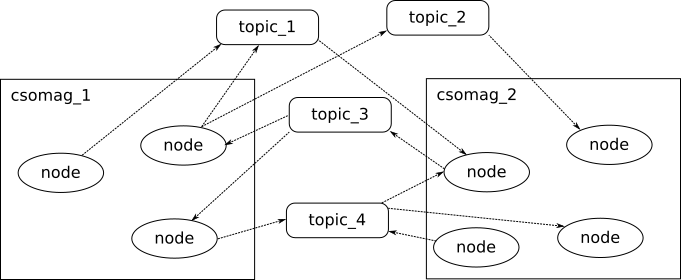
\includegraphics[width=\linewidth]{figures/computational_graph.png}
        \caption{Sematikus ábra}
    \end{subfigure}
    \begin{subfigure}[b]{0.45\linewidth}
        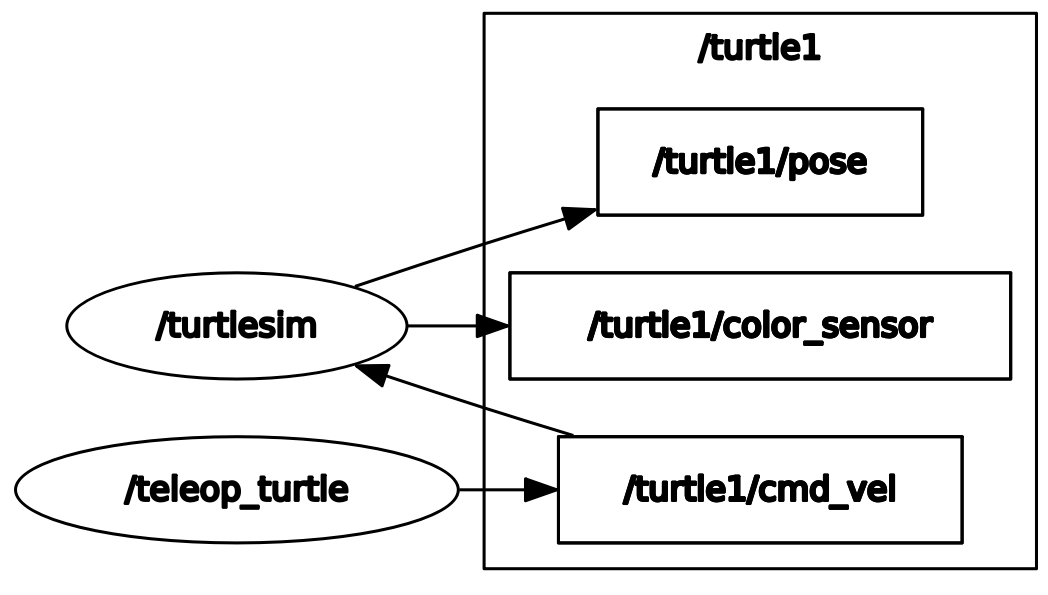
\includegraphics[width=\linewidth]{figures/ros_rqt_graph.png}
        \caption{rqt\_graph}
    \end{subfigure}
    \caption{A komputációs gráf szemléltetése. Bal oldal: sematikus ábra a leírtakról. Jobb oldal: a ROS beépítet \lstinline{rqt\_graph} eszközének kimenete egy egyszerű példán. Oválisok - nodeok, négyszögek - topicok. A \lstinline{turtle1} nagy négyszög egy névteret jelez, mellyel összetartozó topicokat csoportosíthatunk.}
    \label{fig:computational_graph}
\end{figure}

Az így megvalósított rendszer előnye, hogy független végrehajtást tesz lehetővé az alegységek között. Ez azt jelenti, hogy a topicok neveinek egyeztetésével különböző szenzoros és feldolgozó egységek csatolhatóak egymáshoz. Ez azért lehetséges, mert a nevek terminálon keresztül történő újradefiniálását minden ros klienskönyvtár beépítetten támogatja. Így például amennyiben megvalósítunk egy gyorsabb arcfelismerésre képes nodeot az azt megelőzőt könnyűszerrel leválthatjuk. 

A kommunikációhoz használt protokoll legtöbbször a TCPROS\cite{noauthor_rostcpros_nodate}, mely standard TCP/IP socketeket használ, így a robot részei közötti kommunikáció mellett robot-robot kommunikáció is könnyen megvalósítható.

\subsection{Közösségi szint}

A ROS alapvetően szabad szoftver\cite{noauthor_what_nodate}, bár a pontos licenszelése könyvtáranként változó és mint az ilyeneknél jellemző, fejlesztésének jelentős része közösségi alapon folyik. A közösségi szint a különböző ROS disztribúciókat,  repositorykat, a ROS Wikit\cite{noauthor_ros-wiki_nodate}, a ROS Discourse fórumot\cite{noauthor_ros-discourse_nodate}, a ROS Answers Q\&A oldalt\cite{noauthor_ros-answers_nodate} és levelezési listákat. A felsoroltak célja, hogy lehetővé tegyék a különböző szoftverek, tudás és ötletek cseréjét a fejlszetőcsoportok, kutatók és hobbiisták között. A ROS disztribúciói a Linux disztribúciókhoz hasonlóan verziószámmal ellátott szoftvercsomagokat jelentenek, melyek lehetővé teszik, hogy a felhasználók egy tesztelt és működő kódbázisra építhessék projektjeiket. Ennek köszönhetően egy újabb ROS verzió megjelenése esetén is az előző verzió(ka)t használva tovább működhetnek a rá épülő applikációk, időt adva a független fejlesztőknek kódbázisuk frissítésére.

A közösségi részvétel maximalizálása érdekében a ROS föderált tároló modellt követ. Ez azt jelenti, hogy a felhasználókat és a fejlesztőket arra ösztönzik, hogy ROS-csomagjaikhoz saját maguk üzemeltessék tárolóikat. Így a tárolókat karbantartóik tetszés szerint licenszelhetik és kezelhetik, megtartva a kód tulajdonjogát.

A fejlesztés során a leghasznosabb oldalak a ROS Wiki és a ROS Answers. Az elsőn a fejlesztők projektjeik népszerűsítéshez és dokumentációjához hozhatnak létre oldalakat, így igen részletes katalógust biztosít, mikor különböző feladatokat ellátó csomagokat keresünk. A a Stack Overflowhoz hasonló második egy Q\&A (Kérdés és Válasz) típusú oldal, melyen számtalan gyakran felmerülő problémára találhatunk választ és amennyiben ez nem sikerül magunk is feltehetünk kérdéseket.    % Irodalom
\chapter{Szimulációs környezet fejlesztése}
A munka fő célja a roboton futó arcfelismerő modul gyorsabbá tétele volt. Egy program futása több módon is gyorsítható. Egyik alapvető módszer lehetne erősebb hardvert alkalmazni. Ezt esetünkben két okból kiindulva elvetettem. Egyik ok, hogy a hardver adott. A robot segítségével a diplomamunkám folytatása által átölelt időszakban is aktívan kísérletsorozatot végeztek. Másik ok, hogy amennyiben esetlegesen hardveres bővítést végzünk a roboton, akkor annak két töltés közötti hasznos ideje valamilyen mértékben mindenképpen csökkenni fog. Ezeket a szempontokat és hogy a roboton jelenleg képes futni egy kezdetleges megoldás figyelembe véve a hardveres bővítések ötletét első körben elvetettem.

Amennyiben a szoftveres oldalt tekintjük szintén több lehetőségünk adódik. Egyik oldalról fejleszthetjük a futtatni kívánt programunkat, jobb algoritmusokat választva. Mivel az előzetes fejlesztések során a cél annak alapvető működőképessége volt, azt a saját leírása szerint "a világ legegyszerűbb arcfelismerő könyvtára"\cite{geitgey_face_recognition_2021} biztosítja. Ennél jobban optimalizált, illetve modernebb megoldást választva vélhetően jelentős javulás érhető el. Az ezzel kapcsolatos munkálatokat a következő fejezetben tárgyalom.

Másik lehetőségünk, hogy a roboton futó egyéb szoftvereket optimalizálva vagy az esetleges feleslegesen futó szoftvereket leállítva a saját programunk számára extra erőforrásokat szabadíthatunk fel. Ennek segítségével azon túl, hogy a feladatunk megoldására extra számítási és/vagy memóriapacitást biztosíthatunk, potenciálisan a robot általános teljesítménye is javulhat.

Mindegyik említett módszer alkalmazásához először a robot megismerése szükséges - mind hardveres, mind szoftveres téren. Nulladik lépésben emiatt a kutatott témakör irodalmi megismerése mellett ezzel foglalkoztam.

Bár az általam végzett fejlesztés szempontjából nem kritikus, mégis hasznosnak ígérkező extra lépés volt szimulációs környezetet biztosítani a robot számára. Erre elsősorban az enyémmel párhuzamosan futó navigációs fejlesztések miatt volt szükség. Emellett hasznosnak ígérkezett esetleges újabb lezárások esetén illetve egyéb, távmunkát igénylő esetekre, mint például egy külföldi hallgató becsatlakozása.

\section{A robot felépítése}
A robot alapját egy RB-1 BASE henger alakú mobil platform képzi. Átmérője 500mm. USB, Ethernet és HDMI portokkal rendelkezik. Wifi segítségével vezeték nélküli kommunikácóra is képes. 50kg súly elszállítására képes, két töltés közötti üzemideje 10 óra. A benne elhelyezett számítógép Intel i5-ös processzorral és 8 Gb memóriával rendelkezik, melyen 16-os verziószámú Ubuntu Linux rendszer fut. Az alap részletes specifikációi a
\ref{tab:rb1_base_specifications}. táblázatban találhatóak.

\begin{table}[!ht]
    \footnotesize
    \centering
    \renewcommand{\arraystretch}{1.5}
    \begin{tabular} {|r | l |}
        \hline
        Méret & 500 x 215 mm \\
        \hline
        Súly & 30kg \\
        \hline
        Teherbírás & 50kg \\
        \hline
        Sebesség & 1.5 m/s \\
        \hline
        Üzemidő (két töltés között) & 10 óra \\
        \hline
        \hline
        Processzor & Intel i5 \\
        \hline
        Memória & 8 Gb \\
        \hline
        Portok száma & 2 x USB, 1 x Ethernet, 1 x HDMI \\
        \hline
        \hline
        Operációs rendszer & Ubuntu 16 \\
        \hline
        ROS verzió & Kinetic Kame \\
        \hline
        Vezeték nélküli kommunikáció & WiFi 802.11n \\
        \hline
    \end{tabular}
    \caption{Az RB-1 base scpecifikációi.}
    \label{tab:rb1_base_specifications}
\end{table}

Biscee fejlesztése során a paltform egy felépítménnyel és több hardveres kiegészítéssel is el lett látva. A felépítmény anyaga alumínium, fő részei a robothoz rögzített oszlop és az ehhez az oszlophoz derékmagasságban csatlakozó hordtálca. A hordtálca anyaga fa. Mivel a robot wifi jelét a beépített router helyzete miatt jelentősen árnyékolja a felépítmény alatt egy kisméretű switch hub lett elhelyezve. A hordtálca kerülete mentén 7 ultrahang szenzor lett elhelyezve, ebből 6 navigációs, 1 pedig kommunikációs célt szolgál. A szenzorok értékeit Arduino mikrokontrollerek olvassák ki, az értékeket USB-n keresztül továbbítják a robot számára egy USB hubon keresztül. A robot kamerái az oszlop tetején kialakított fejrészen helyezkednek el. A fejrész mozgatását két DYNAMIXEL szervó teszi lehetővé. A kábelezés eltakarása és a természetes hatás keltésének érdekében a robotot műbőr borítással látták el. A hordtálcáról lelógó csíkozott műbőr szoknya könnyű hozzáférést biztosít a hubokhoz és a kábelezéshez. A leírtak megfigyelhetőek a
\todo{ábra}. ábrán.

\section{ROS, szimulációs és virtualizációs lehetőségek}
A roboton a Robot Operating System (ROS) Kinetic Kame verziója fut. Bár a ROS elviekben bármilyen Linux alapú rendszeren, illetve akár Windows alatt is futtatható, hivatalos kiadásai szorosan kötődnek az Ubuntu Linux operációs rendszerhez. A napjainkra már EOL (End Of Life - élete végére ért) Kinetic Kame kiadás az Ubuntu 16 (Xenial Xerus) LTS (Long Term Support - hosszú támogatási idejű) verziójához jött ki, mely mára szintén EOL rendszer. Ez szempontunkból azért különösen lényeges, mert a szimuláció fejlesztésekor a felhasznált csomagok verzióinak egyeztetése szükséges. Szerencsére mára több virtualizációs lehetőség is létezik, melyek segítségével direkt telepítés nélkül is képesek vagyunk egy bizonyos operációs rendszer futtatására. A szimuláció fejlesztése elosztott feladatként folyt. A robot felépítményéről 3D modell készült, a robot teszteléséhez használt teremről pedig gazebo világ. Ezek a \ref{fig:3d_model_and_gazebo_world}. ábrán láthatóak. A diplomamunka részfeladatának tárgyát az RB-1 Base létező szimulációjának ezekkel és a hozzáadott szenzorokkal történő kiegészítése képzi. A fejlesztési környezet az alacsony belépőszint és könnyű megoszthatóság miatt egy Oracle VM Virtualbox\cite{noauthor_oracle_nodate} virtuális gépen történt. A szimuláció továbbá tesztelten sikeresen futtatható WSL\cite{craigloewen-msft_wsl_nodate} alatt és konténerizálva Docker\cite{noauthor_docker_nodate} vagy SingularityCE\cite{noauthor_singularityce_nodate} alatt.

\begin{figure}
    \centering
    \begin{subfigure}[b]{0.45\linewidth}
        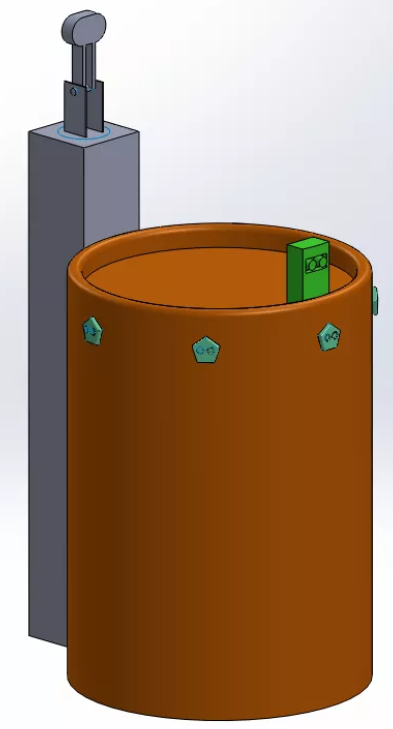
\includegraphics[height=7cm]{figures/biscee_model.png}
    \end{subfigure}
    \begin{subfigure}[b]{0.45\linewidth}
        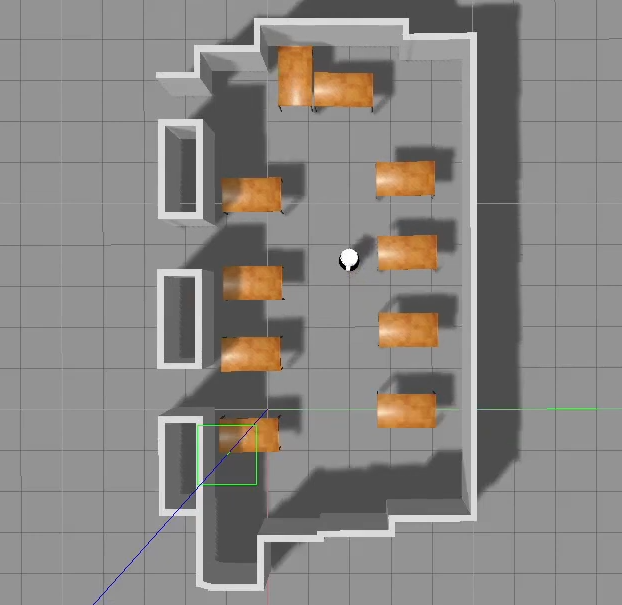
\includegraphics[width=\linewidth]{figures/simulation_from_above.png}
    \end{subfigure}
    \caption{A szimulációhoz készült 3D modell és Gazebo world.}
    \label{fig:3d_model_and_gazebo_world}
\end{figure}

A ROS beépített fizikai szimulációra alkalmas környezetet nem tartalmaz. A legelterjedtemm megoldás erre a Gazebo robotszimulátor alkalmazása. A \lstinline{gazebo_ros_pkgs} metacsomag által rendelkezésünkre álló wrapperek segítségével könnyen hozhatunk létre és indíthatunk el ROS-on belülről robotmodelleket és szimulációkat.

A Gazebo a szimulációk leírásához SDF (Simulated Description Format) fájlokat használ, mely egy objektumok, környezetek és az ezek közötti kapcsolatok leírására specializált XML formátum. Ezzel szemben a ROS a robotok leírásához az URDF (Universal Robotic Description Format) formátumot használja. Amint neve sugallja, ez az előzővel szemben robotok leírására alkalmas. Szerencsére az ezek közötti konverzió megoldott, ezért elegendő az utóbbit létrehoznunk. Az egyszerűbb kezelhetőség érdekében lehetőségünk áll továbbá xacro makrók használatára. A leírtak és az URDF működésének szemléltetésére jó példa az eredeti robot szimulációjának kiegészítése az elkészült 3D modellel és ultrahang szenzorokkal. Az urdf tartalmának a \lstinline{<robot>} tagen belül kell elhelyezkednie. A többször használandó értékeket definiálhatjuk \lstinline{xacro:property}ként, így azokat globálisan tudjuk állítani esetleges változás vagy elírás esetén. 
\lstinputlisting[language=XML]{figures/code/urdf_xacro_basic.xml}
A robotunkat jointokból (csukló) és linkekből (tag) építjük fel. Az eredeti robot rendelkezik egy bázisként szolgáló taggal, először ehhez írunk le egy kapcsolatot egy csukló segítségével. Ehhez először meg kell adnunk ennek típusát és helyzetét. Esetünkben ez egy fix eltolást jelent a bázistól, ezért típusink "fixed" és az \lstinline{origin} tagen belül egy z irányú eltolást definiálunk. Ezt követően megadjuk a csuklót követő és az az előtti tagokat a \lstinline{child} és a \lstinline{parent} tagek segítségével.
\lstinputlisting[language=XML]{figures/code/urdf_joint.xml}
A tagok leírása kissé hosszabb, hiszen ezek képzik a robotunk fizikai elemeit. Itt kell megadnunk a részek inerciális értéket. Fontos részleg, hogy a részek számár külön definiálhatunk ütközési alakot és vizuális kinézetet. Ezek közül mindkettő \lstinline{geometry} tagek segítségével történik. Használhatunk egyszerű alakzatokat, mint téglatestek vagy hengerek. Amennyiben az adott rész alakja jól közelíthető ezek valamelyikével érdemes lehet ütközési alakzatként azt alakamaznunk. Használhatunk továbbá egyedi modelleket is a \lstinline{mesh} tag segítségével.
\lstinputlisting[language=XML]{figures/code/urdf_link.xml}
A szenzorok definíciója a \lstinline{gazebo} taggel történik. Ennek meg kel adnunk, mely tagunkhoz tartozik a szenzor. Ez után következnek a szenzorhoz tartozó tulajdonságok leírásai, egy UH szenzor esetén ez a kibocsájtott sugárzás. Meg kell adnunk továbbá a szimulációhoz szükséges gazebo plugint is. Ezen belül definiálhatjuk a szimuláció további részleteit és a szenzorok által használt ROS topicokat.
\lstinputlisting[language=XML]{figures/code/urdf_gazebo.xml}
Amennyiben megírtuk a szükséges kiegészítéseket, az ezeket tartalmazó filet xacro segítségével egyszerű beemelhetjük a robot eredeti leírásába.
\begin{lstlisting}
    <xacro:include filename="$(find rb1_base_description)/urdf/custom_stuff/custom_stuff.urdf.xacro"/>
\end{lstlisting}
Az újrahasználhatóság és az egyszerű konfiguráció érdekében saját makrókat is létrehozhatunk. Esetünkben például a bisceen használt ultrahang modulokhoz ez előnyös megoldás volt, hiszen 6 ugyan olyan szenzor is elhelyezésre került különböző pontokon. A makrók számára paraméterek adhatóak meg, melyek segítségével az adott alkalmazás pontosítható.
\begin{lstlisting}
    <xacro:macro name="sensor_biscee_ultrasound" params="prefix parent prefix_topic:='uh' *origin min_angle:=-0.14835 max_angle:=0.14835 uh_fov:=0.2967 gpu:=^|true">
\end{lstlisting}
A szenzorokat ezt követően egyszerűen hozzáadhatjuk a robot leírásához.
\begin{lstlisting}
<xacro:sensor_biscee_ultrasound prefix="$(arg prefix)front_bottom_ultrasound" parent="$(arg prefix)base_link" prefix_topic="/front_bottom_ultrasound">
    <origin xyz="0.223 0.0 1.159" rpy="0 3.1416 3.1416"/>
</xacro:sensor_biscee_ultrasound>
\end{lstlisting}
A szimuláció az \lstinline{rb1_base_sim} csomag segítségével futtatható. Megfelelően átkonfigurálva és a bisceet indító launch fileba illesztve a szimuláció egyetlen \lstinline{roslaunch} parancs futtatásával elindítható. A szimuláció során a beépített rViz\cite{noauthor_rviz_nodate} vizualizáció is fut, melynek segítségével a robot által érzékelt környezetet és útvonaltervezést ellenőrizhetjük. A szimuláció futás közben a \ref{fig:simulation_gazebo_and_rviz}.ábrán látható Szükség esetén akár saját navigációs pontot is hozzáadhatunk.

\begin{figure}
    \centering
    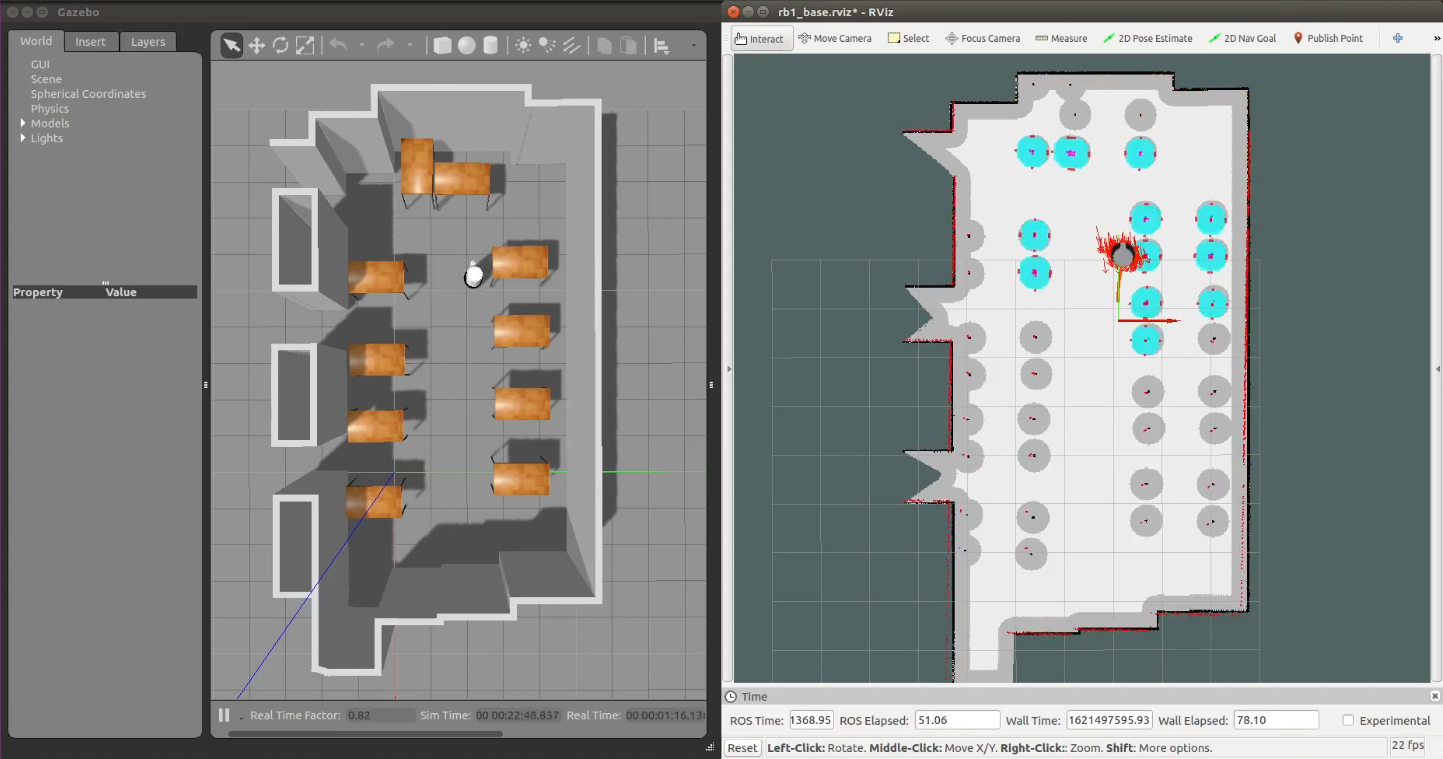
\includegraphics[width=\linewidth]{figures/simulation_gazebo_and_rviz.png}
    \caption{Gazebo szimuláció és rViz.}
    \label{fig:simulation_gazebo_and_rviz}
\end{figure}

Sajnos a fejlesztés során kiderült, hogy a kamerák szimulációja sem virtuális gépen, sem konténerben futtatva nem működőképes. Ennek ellenére a szimuláció fejlesztése nem csak az egyéb fejlesztésekhez, hanem számomra is hasznosnak bizonyult, mivel menet közben megismertem a nodeok konténerben futtatásának lehetőségét. Ez lehetőséget biztosít, hogy a roboton futó régi operációr rendszer ellenére újabb rendszereken elérhető megoldásokat alkalmazzunk.

\chapter{A potenciális algoritmusok kiválasztása}

A fejlesztői munka természeténél fogva iteratív. Első lépésként a roboton jelenleg futó megoldásból és internetes keresés alapján meghatároztam a potenciális algorimusokat. Ezt követően felkutattam ezek létező implementációit. Ezt felhasználva előzetesen rögzített és élő kameraképet feldolgozva először előzetes szűrést végeztem pontatlan és/vagy lassú megoldások kiszűrésére. Lévén az egyes cikkek és git repositoryk gyakran egymásra hivatkoznak vagy több algoritmust/implementációt is tartalmaznak az implementáció-tesztelés és az irodalmi kutatás egymáshoz viszonyított helyzete változó volt. Az írott forma átláthatóságát az ily módon történő tárgyalás jelentősen akadályozná, ezért a következőkben az algoritmusokat és keretrendszereket általam választott sorrendben tárgyalom. Fontos továbbá megemlíteni, hogy az egyes algoritmusok és az alkalmazott keretrendszerek/könyvtárak neurális hálózatok esetén legtöbbször egymástól függetlenek. Egy tetszőlegesen választott struktúrát implementálhatunk Caffe, Pytorch és Tensorflow segítségével is. A választás során ezért előnyben részesítettem azokat az implementációkat, melyek lehetőleg a képek kinyerésére amúgy is felhasznált OpenCV könyvtárat használják, hiszen ez emiatt előre telepítve van a roboton. ROS nodeokat implementálhatunk mind C++, mind Python nyelven. Bár C++ használatával vélhetően kismértékben gyorsabb implementációk lennének létrehozhatóak, a könyvtárak verzióinak változására tapasztalataim szerint érzékenyebb, nehezebben frissíthető kódot kapunk.

Jellemző probléma volt az egyes megoldások, de még inkább az egyes kiértékelő programok esetén a verziók egyeztetése. A Python által nyújtott virtuális környezetek és csomagkezelés rugalmas megoldást képesek nyújtani ennek kiküszöbölésére. C++ esetén a legjobb megoldásnak a szimulációnál már bevált Docker konténerek alkalmazása bizonyult.

\section{Az algorimusok előzetes értékelése}
Az összehasonlításhoz először azonosítani kell a jelölteket. Az arcdetekció extenzív irodalommal rendelkezik, így nagy létszámú jelöltből kell választanunk. Ezen lépés célja, hogy feltárja azokat a megoldásokat, amelyek potenciálisan kielégítik az adott feltételeket. Ezek közül esetünkben a legfontosabb a jelenleginél nagyobb sebesség biztosítása legalább összemérhető pontosság mellett. Fontos továbbá, hogy rendelkezésünkre álljon az algoritmus valamilyen mértékű implementációja, hiszem a magas számú jelölt miatt nem áll rendelkezésünkre az idő és a tanításhoz szükséges számíási kapacitás sem.

A ROS \lstinline{cv_bridge} csomagja segítségével rendelkezésünkre áll az OpenCV\cite{noauthor_opencvopencv_2021} könyvtárral való együttműködéshez szükséges interfész, mely a roboton előzetesen is rendelkezésre áll. Ebből kifolyólag és a széleskörű elterjedtségének köszönhetően ezt a könyvtárat választottam képfeldolgozáshoz. Segítségével könnyen olvashatunk be képeket és videókat, a számtalan beépített konverziós függvény segítségével pedig könnyen létrehozhatjuk az különböző igényelt bemeneteket. Könnyen kezelhetjük továbbá a számítógéphez csatlakoztatott webkamerákat, ami a választás során igen hasznosnak bizonyult. Élő kamerakép segítségével gyorsan és rugalmasan tesztelhetjük a talált algoritmust, előzetes képet kapva annak sebességéről és a felismerés limitációiról. A \ref{fig:selection_webcam}. ábrán látható példán például az első esetben az algoritmus sikeresen felismeri a frontális és profilnézetű arcot is, viszont a második esetben látható, hogy a jelentősen oldalra fordított frontális arcot már nem képes detektálni. Amennyiben az algoritmust több személy detektálására kívánjuk tesztelni partner vagy a képen látható módon képes segítségével is megtehetjük. Az előre elkészített képekkel szemben ez a módszer ennél a lépésnél előnyt jelent, mert a teszt az eredményektől függően könnyedén, adaptívan változtatható. Emellett az ember számára könnyen feldolgozható információt biztosít az algoritmus sebességéről is.

\begin{figure}
    \centering
    \begin{subfigure}[b]{0.45\linewidth}
        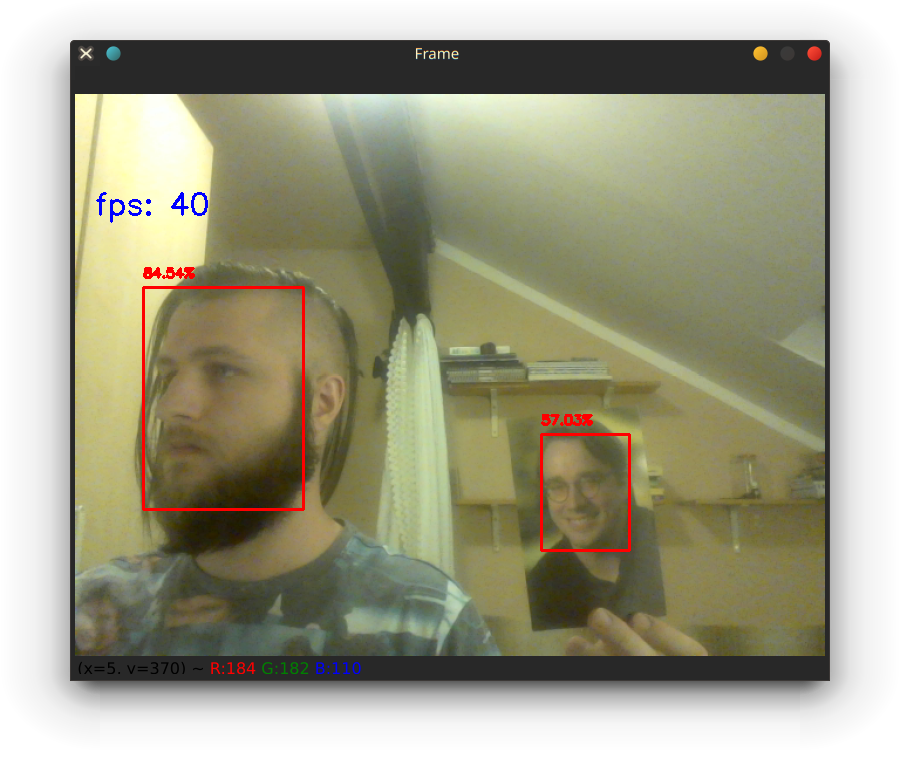
\includegraphics[width=\linewidth]{figures/selection_webcam_linus_good.png}
    \end{subfigure}
    \begin{subfigure}[b]{0.45\linewidth}
        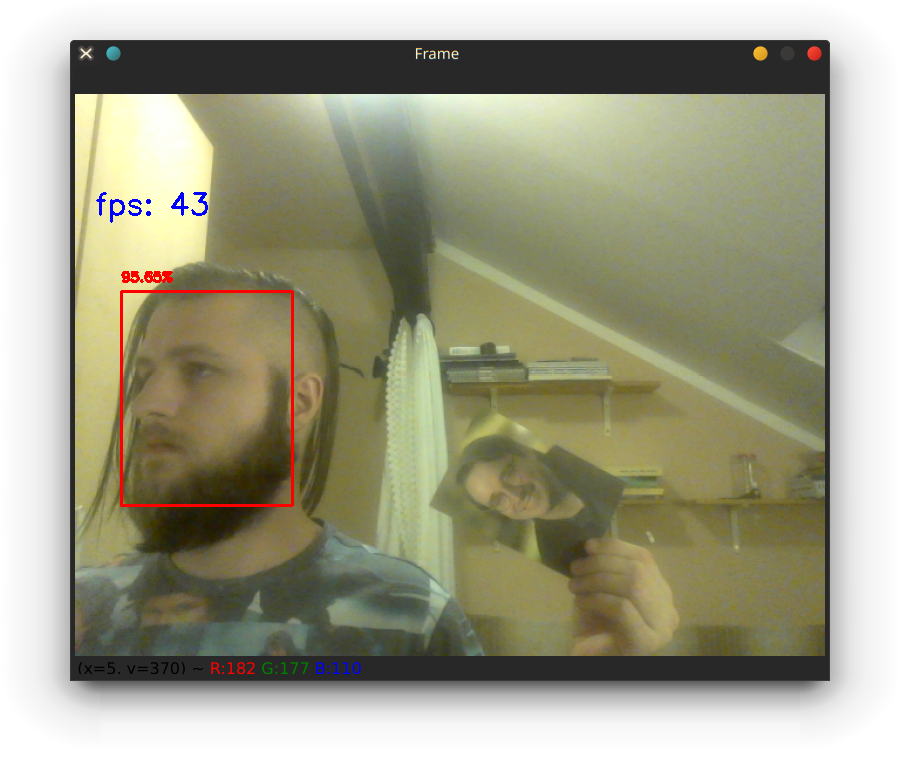
\includegraphics[width=\linewidth]{figures/selection_webcam_linus_bad.png}
    \end{subfigure}
    \caption{Algoritmus tesztelése webkamera segítségével.}
    \label{fig:selection_webcam}
\end{figure}

\section{HAAR kaszkád (OpenCV)}
Alapja a Viola és Jones által “Rapid Object Detection using a Boosted Cascade of Simple Features”\cite{viola_rapid_2001} című cikkükben bemutatott és “Robust Real-Time Face Detection”\cite{viola_robust_2004} című cikkükben (közel) valós idejű arcdetekcióra alkalmazott algoritmus. A módszer működésének alapját az irodalmi áttekintésnél már ismertettem.

Annak ellenére, hogy két évtizedes technológiáról beszélünk, alkalmazása még ma is igen elterjedt. Régebbi vagy akár mai olcsóbb videokamerák és fényképezőgépek ezt a módszert alkalmazzák. A ROS egyetlen hivatalos arcfelismerő csomagja \cite{noauthor_face_detector_nodate} is kaszkád alapú.

Az OpenCV könyvtár beépített példái között több arcfelismerésre alkalmazható kaszkádot is találhatunk. Ezek leírását xml fájlok tartalmazzák, melyeket megtekinthetünk a hivatalos Github repositoryban\cite{noauthor_opencvopencv_2021}, a \lstinline{data/haarcascades} mappa alatt. A módszer fő hátulütőjéről előzetes sejtést adhat, hogy találhatunk \lstinline{haar_frontalface.xml} és \lstinline{haar_profileface.xml} verziókat, de egybevontat nem. A fileokat megtekintve megtudhatjuk továbbá, hogy a kaszkádok függőleges arcokat feltételeznek.

\section{HoG (Dlib)}
\todo{megírni}
A roboton jelenleg futó algoritmus. Az alap szint, melyet a jelölteknek el kell érnie.

\section{ResNet-10 SSD (OpenCV Caffe)}
A háló ötvözése a "SSD: Single Shot MultiBox Detector"\cite{liu_ssd_2016} és "Deep Residual Learning for Image Recognition"\cite{he_deep_2015} cikkekben bemutattott módszereknek. Az SSD módszer három fő alrészre bontható, melyek a
\ref{fig:ssd_multibox_detector}
ábrán láthatóak. A módszer alapját konvolúciós rétegek képzik.

\begin{figure}
    \centering
    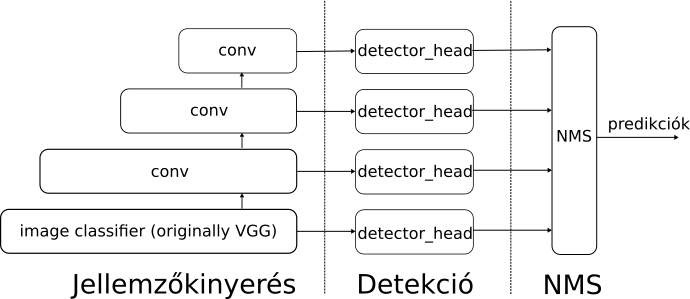
\includegraphics[width=\linewidth]{figures/ssd_multibox_detector.png}
    \caption{SSD MultiBox detektor sematikus ábrája}
    \label{fig:ssd_multibox_detector}
\end{figure}

Első lépése a jellemzők kinyerése, mely lényegében képosztályzást jelent. Bemenete egy kép, melyre tekinthetünk egy 3 csatornás feature mapként (jellemző térkép). Kimenete jellemzően kisebb méretű, ám jóval több csatornából áll. Ezt az eredeti megoldásban egy VGG\cite{simonyan_very_2015} hálózatra alapozták. A különböző méretű detekciók végrehajtásának érdekében még a jellemzőkinyerés lépésén belül a kinyert jellemzőket további konvolúciós hálózatok piramisán küldjük keresztül, melyek egyre kisebb méretű kimenetekkel rendelkeznek. A köztes kimeneteket eltároljuk a következő lépés számára.

Második lépésben következik a detekciós fázis. A módszer fix számú alapvető predikciós dobozt feltételez, melyet jelöljünk \(n_A\)-val. Ezek a dobozok a konvolúciós viselkedésnek megfelelően csempézik ki a képet. A detektoraink generált feature mapenként minden dobozhoz két kimenetet generálnak. Az első az objektumosztályoknak megfelelő \(n_C\) darab konfidencia értéket tartalmazza. A második dobozonként 4 transzformációs értéket a doboz (x, y) pozícióját és (h, w) magassát és szélességét illetően, a detekció pontosításának érdekében.

Harmadik lépésben NMS-t (Non Maximum Supression) végzünk a többszörös detekciók kiküszöbölésének érdekében. Ennek oka, hogy a különböző méretű és alakú dobozok közül várhatóan egy-egy objektumot többön belül is érzékelni fogunk. Ennek érdekében a nagyban átfedő négyzetek közül csak a legmagasabb konfidencia értékkel rendelkezőt tartjuk meg.

\section{FaceBoxes (Pytorch)}
A "Faceboxes: A CPU real-time and accurate unconstrained face detector" című cikkben tárgyalt algoritmus két fő részre osztható, melyek megfigyelhetőek a
\ref{fig:faceboxes}. ábrán.

\begin{figure}[h]
    \centering
    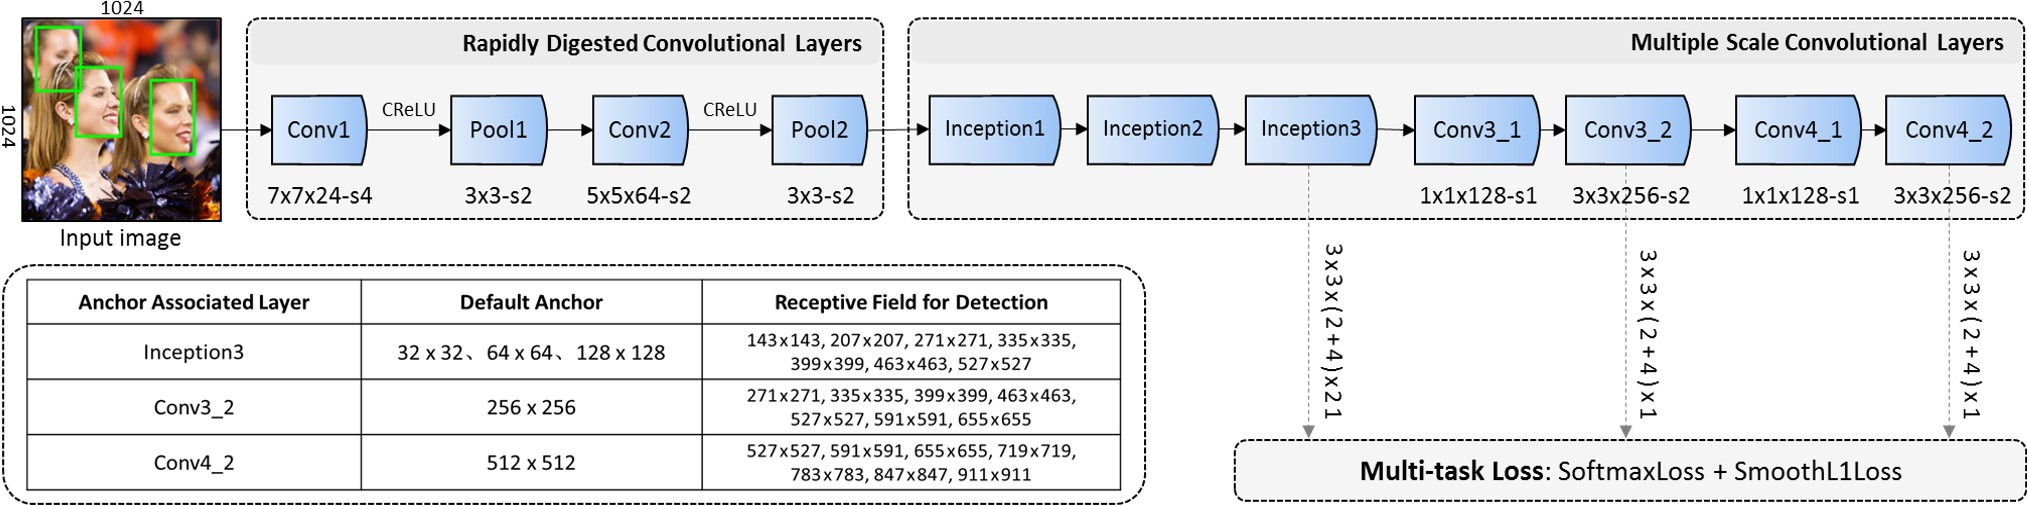
\includegraphics[width=\linewidth]{figures/faceboxes_framework.jpg}
    \caption{A faceboxes algoritmus felépítése. Az ábra az eredeti cikkhez\cite{zhang_faceboxes_2018} tartozó hivatalos github repositoryból\cite{zhang_faceboxes_2021} adoptálva.}
    \label{fig:faceboxes}
\end{figure}

Az első, a Rapidly Digested Concolution Layers (RDCN, "Gyorsan Emésztett Konvolúciós Rétegek") nevet kapta. Fő észrevétele, hogy a nagy bemenet, kernelméret és kimenetből adódó, a CNN alapú megoldásokra jellemző lassúság megfelelően beállított paraméterek segítségével végrehajtott gyors dimenziócsökkentéssel kiküszöbölhető. Ez különösen nagy előnyt jelent CPU-n történő futtatáskor, mely tervezett felhasználási módunk számára elsődleges szempont. Másik fontos része ennek a lépésnek a C.ReLU \cite{shang_understanding_2016} aktivációs függvény alkalmazása, melynek lényege, hogy a kimenet negáltját hozzáfűzi az eredeti kimenethez. Ez igen olcsó művelet és kiküszöli a CNN-ekre jellemző szimmetrikus kimenetek betanulását.

A második szakasz a Multiple Scale Convolution Layers (MSCL, "Több Méretű Konvolúciós Rétegek"), mely három ötletet ötvöz. Első lépésben inception \cite{szegedy_going_2015} rétegek segítségével több méretnek megfelelő jellemző reprezentációkat generál a detekciós rétegek számára. Ezt követően a Feature Pyramid Network (FPN) \cite{lin_feature_2017} módszer által inspirálva a durvább felbontású feature mapek értékei bilineáris skálázással felskálázva, majd egy 1x1-es konvolúció segítségével a megfelelő csatornaszámra csökkentve a finomabb felbontásokhoz hozzáadódnak. A különböző rétegek dobozait ezt követően az SSD-hez \cite{liu_ssd_2016} hasonlóan osztják föl.
\todo{ide lehetne még írni a további két lépésről, ha kell}

Az algoritmus eredeti kódja szabadon elérhető a(z) \lstinline{sfzhan15/FaceBoxes} \cite{zhang_faceboxes_2021} Github repository alatt. Elérhető továbbá az előzőleg kifejtettek szempontjából kedvezőbb Pytorch alapú Python implementáció is a \lstinline{zisianv/FaceBoxes.Pytorch} \cite{wong_faceboxes_2021} repository alatt.

\section{BlazeFace (Mediapipe)}
A "BlazeFace: Sub-millisecond Neural Face Detection on Mobile GPUs"\cite{bazarevsky_blazeface_2019} cikk címéhez híven a tárgyalt algoritmus mobil GPU-val rendelkező eszközökre lett optimalizálva. Alapja(i) a MobileNetV2/V2 \cite{howard_mobilenets_2017, sandler_mobilenetv2_2019} algoritmusok, melyek egyébként az SSD-ből GPU barát formára módosított alapvető doboz rendszert alakalmaznak. Ez a \ref{fig:blazeface} látható. ábrán. Ezekhez képest nagyobb kernelméretű konvolúciós rétegeket alkalmaz, melyek GPU-n történő futtatás szempontjából előnyösek, a miénkből pedig sajnos meglehetősen hátrányosak. Ennek ellenére CPU-n is igen kedvező sebességek érhetőek el vele. Az ezekből álló BlazeBlock névre keresztelt egységek a \ref{fig:blazeface}. ábrán láthatóak.

\begin{figure}[h]
    \centering
    \begin{subfigure}[b]{0.45\linewidth}
        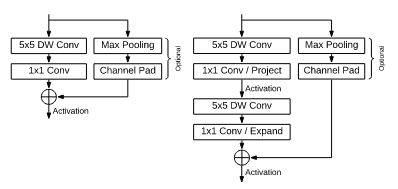
\includegraphics[width=\linewidth]{figures/blaze_block.png}
        \caption{BlazeBlock és dupla BlazeBlock}
    \end{subfigure}
    \begin{subfigure}[b]{0.45\linewidth}
        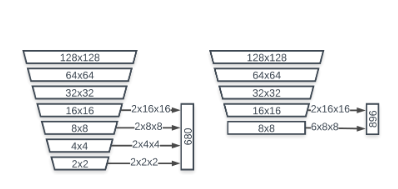
\includegraphics[width=\linewidth]{figures/blazeface_anchor_computation_vs_ssd.png}
        \caption{Előzetes jellemzőkinyerés tradícionális SSD (bal) esetén és a BlazeFace (jobb) esetén.}
    \end{subfigure}
    \caption{A BlazeFace által alkalmazott módosítások. Az ábra az eredeti cikkből\cite{bazarevsky_blazeface_2019} adoptálva.}
    \label{fig:blazeface}
\end{figure}

Az algoritmus kiválasztásának oka a Google MediaPipe\cite{noauthor_mediapipe_nodate} által nyújtott letisztult Python API és előre tanított modellek voltak. 

\section{RetinaFace (insightface)}
A 2019-ben megjelent "RetinaFace: Single-stage Dense Face Localisation in the Wild"\cite{deng_retinaface_2019} cikkben megjelent RetinaFace a legújabb algoritmus a tárgyaltak közül. Ennek köszönhetően az előzőekben tárgyalt módszerek jelentős részének alkalmazása megfigyelhető benne. A publikációban javasolt szerkezet a
\ref{fig:retinaface}. ábrán látható.

\begin{figure}[h]
    \centering
    \begin{subfigure}[b]{\linewidth}
        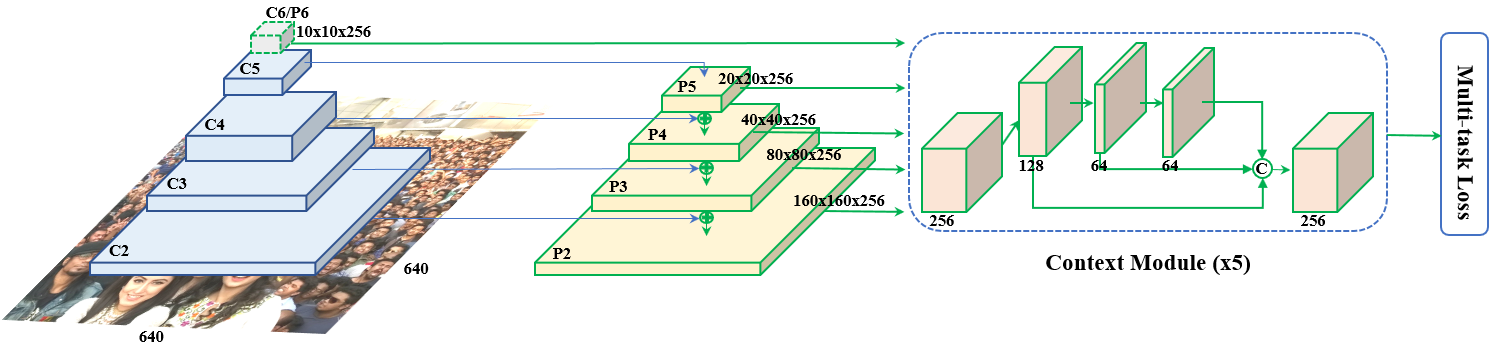
\includegraphics[width=\linewidth]{figures/retinaface_framework.png}
        \caption{Az algoritmus belső felépítése}
    \end{subfigure}
    \begin{subfigure}[b]{0.75\linewidth}
        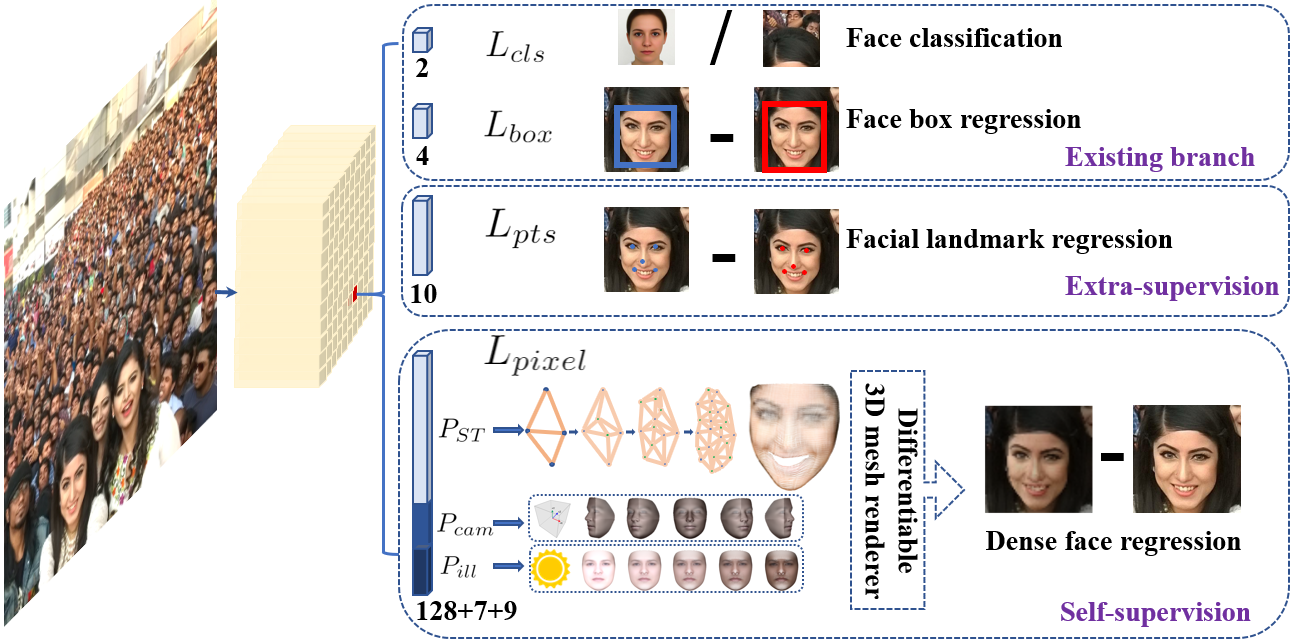
\includegraphics[width=\linewidth]{figures/retinaface_multitaskloss.png}
        \caption{Az algoritmus kimenetei és az alkalmazot multitask loss szemléltetése}
    \end{subfigure}
    \caption{A RetinaFace algoritmus felépítése. Az ábra az eredeti cikkből\cite{deng_retinaface_2019} adoptálva.}
    \label{fig:retinaface}
\end{figure}

A módszer egy 5 szintű FPN inspirált jellemző piramist alkalmaz, melynek bemeneteit már a háló tanítását megelőzően előre betanított ResNet szakaszok biztosítják, ezeket C1-C6-al jelzik.
\todo{ábrához odaírni, hogy C1 omittálva lett róla}
Ebből ötnél a korrábbi megoldásoknál \cite{lin_feature_2017,lin_focal_2018} is használt föntről lefelé haladó és oldalirányú kapcsolatokkal. Ezek az ábrán a P2-P5 jelzésű rétegek. A piramis P6-al jelzett csúcsa egy 3x3-as, 2-es stride értékű konvolúcióval áll elő C5-ből. Mivel nem vesz részt a föntről lefelé csatolásban, ezért C6 jelzéssel is ellátták. Ezt követően az SSH\cite{najibi_ssh_2017} és PyramidBox\cite{tang_pyramidbox_2018} által inspirált, továbbá a 2018-as WIDER Face Challenge győztesének megoldása\cite{loy_wider_2019} alapján módosított kontextus modulokat alkalmaznak a piramis öt szintjére, ezzel növelve az érzékelőmezőt és a rigid kontextusmodellezési erőt.

Az algoritmus kiválasztásának oka a papír által ígért a technika jelenlegi állása szerint a legjobbak között szereplő pontosságán és sebessén túl az volt, hogy implementációi rendelkezésre állnak Pytorch\cite{biubug6_retinaface-pytorch_2021} és Tensorflow\cite{stan_btd_retinaface-tf2_2021} keretrendszerekre is. Az algoritmus eredeti implementációjából kinőtt InsightFace\cite{noauthor_insightface_nodate} projekt szabad szoftverként MIT Licensz alatt biztosít hozzáférést \cite{noauthor_insightface-github_2021} a mai napig folyamatosan fejlesztett modelljeikhez, melyekhez kényelmes Python könyvtár is tartozik. Amennyiben szükség és lehetőség lenen rá, a könyvtár az előre betanított algoritmusokon túl továbbtanítási lehetőséget is ad. Emellett az arcdetekción túl state-of-the art arcfelismerési algoritmusokat is rendelkezésünkre bocsájt, melyek szintén egyszerűen tovább taníthatóak. A projektre napjainkban még nem kifejezetten könnyű rátalálni, azonban a jövőben számos kis fejlesztői csapat és open source projekt létrejöttét segítheti.

\chapter{A kiválasztott algoritmusok értékelése}
A webkamerás tesztelés betekintést enged az egyes módszerek erősségeibe és hátrányaiba, azonban két jelentős limitációval is rendelkezik. Egyrészt az eredmények nem számszerűsíthetőek, ezért hasonló teljesítményű megoldások közötti választáskor nem tudunk objektív döntést hozni. Másfelől a robot kamerái a webkameraképtől több területen jelentősen különbözhetnek, mint például annak felbontása és színösszetétele. Emellett a robot feladatának teljesítése közben mozgásban van, így például a képek megvilágítása is folyamatosan változhat.

\section{Benchmark alapú összehasonlítás}
Az algoritmusok objektív összehasonlításához teszteket végeztem a korábban ismertetett benchmarkokon. A fellelhető implementációk gyakran jelentős eltérést mutatnak a publikációkban tálalt eredményekhez képest. Ennek egyik vélhető oka, hogy a gépi tanítási folyamatok sok finomhangolást igényelnek az optimális eredmények eléréséhez. A tanítási folyamat más megoldásoktól eltérő pontjai legtöbbször szerepelnek a cikkekben, az ilyen részletek azonban sokszor kihagyásra kerülnek. Emellett a véletlen inicializációnak köszönhetően akár ugyan olyan paraméterek mellett, ugyan azon a gépen futtatva a tanítást két különböző időpontban különböző eredményeket kaphatunk. Másik tényező a különböző keretrendszerek jelenléte. Az implementációt megvalósító programozó tudásától és az alkalmazott segédeszközöktől függően különbségek tapasztalhatóak azok átláthatóságában, pontosságában és sebességében.

\paragraph{ROC}\hfill

Az arcdetekció bináris klasszifikációs feladat, melyhez jellemzően két kiértékelési módszert alkalmaznak. Az első a Receiver Operating Characteristic (ROC) görbe. Ennek x tengelyén a hamis pozitívak rátája, más néven 1 - specificitás található. Ez nevéből sejthetően azt adja meg, milyen gyakran osztályzunk hibásan pozitívként egy egyébként negatív példát, melyet a következőképp számolhatunk:

\begin{equation}
    HPR = 1 - specificitás = \frac{HP}{HP + IN}
\end{equation},
ahol
\begin{itemize}
    \item HP a hamis pozitívok száma
    \item IN az igaz negatívok száma
\end{itemize}

Az y tengely értékeit az igaz pozitívok rátája, más néven a szenzitivitás adja. Ez azt számszerűzíti, milyen arányban ismerünk fel egy pozitív esetet valóban pozitívként. A következő módon számolhatjuk:

\begin{equation}
    IPR = szenzitivitás = \frac{IP}{IP + HN}
\end{equation},
ahol
\begin{itemize}
    \item IP az igaz pozitívok száma
    \item HN a hamis negatívok száma
\end{itemize}
A görbe egy pontját ezekből úgy kaphatjuk, hogy az összes predikciónkból valamilyen konfidenciaszint szerint kiválasztott halmazra kiszámoljuk és ábrázoljuk őket. Ez után a konfidenciaszintet variálva kiszámolhatjuk a többi pontot is. A klasszifikátorok pontozása a görbe alatti terület értékével történik, a nagyobb érték jobb. A módszer szemléltetése a \ref{fig:roc}. ábrán látható. A valós megoldások többnyire a véletlen találgatás (AUC = 0.5) és a tökéletes klasszifikátor (AUC = 1) között helyezkednek el, de létezhet 0.5 alatti pontszám is.

\begin{figure}
    \centering
    \begin{subfigure}[b]{0.45\linewidth}
        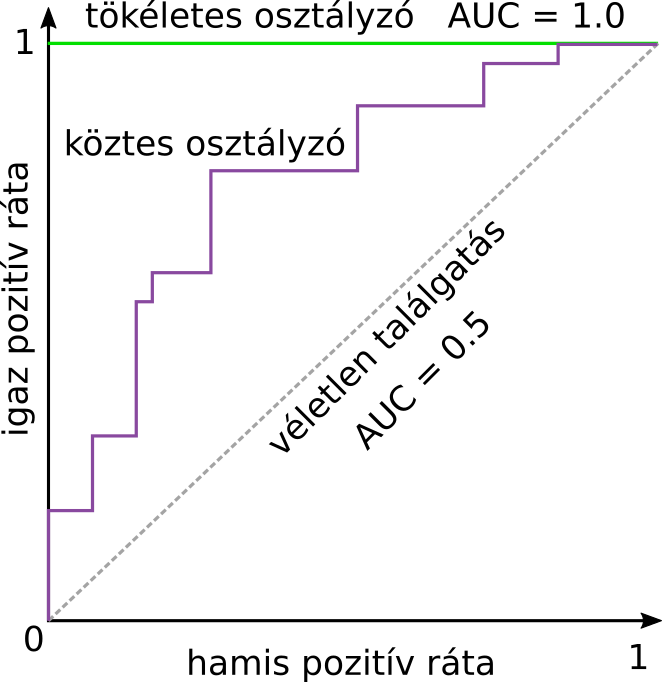
\includegraphics[width=\linewidth]{figures/ROC.png}
        \label{fig:roc}
    \end{subfigure}
    \begin{subfigure}[b]{0.45\linewidth}
        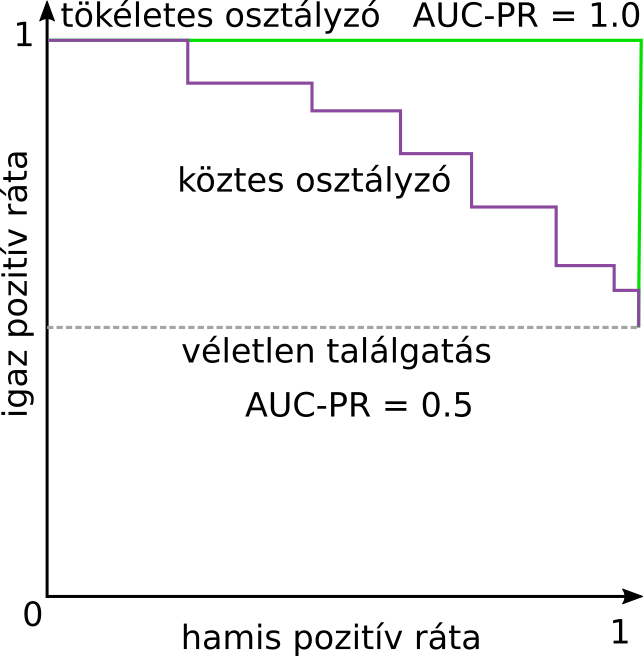
\includegraphics[width=\linewidth]{figures/PR.png}
        \label{fig:pr}
    \end{subfigure}
    \caption{ROC(bal) és PR(jobb) görbék.}
    \label{fig:roc_and_pr_curves}
\end{figure}

\paragraph{Precision - Recall}\hfill
A másik gyakran alkalmazott módszer a Precision - Recall görbe. Ennek tengelyei a nevében található értékek, melyeket az előzőekben használt jelölésekkel a következő módon kaphatunk meg:
\begin{equation}
    precision = PPE = \frac{IP}{IP + HP}
\end{equation}
\begin{equation}
    recall = szenzitivitás =  \frac{IP}{IP + HN}
\end{equation}
Amint látható a recall egyenlő a ROC görbénél alkalmazott szenzitivitással. A precíziót nevezhetjük még Pozitív Predikciós Értéknek (PPE) is. Értelmezése az, hogy a pozitív predikcióink mekkora részben tartalmaznak valóban pozitív eseteket. A gráf egyes pontjait a ROC-hoz hasonlóan kaphatjuk. Pontozása szintén megfeleltethető a görbe alatti területnek. Ezt legtöbbször az Átlagos Precízió (AP) számításával érik el úgy, hogy az egyes konfidenciaszintek precision értékét súlyozottan átlagolják.

\section{Összehasonlítás a robotról származó felvételeken}
A benchmark alapú összehasonlítás jó és számszerűsíthető értékelést ad az algoritmusok pontosságáról, azonban nem biztosít átfogó képet azok előnyeiről és hátrányairól specifikus felhasználási esetekben. Ez alól valamelyest kivételt képez a WIDER face adatszett, amely események szerint szeparálva tartalmaz képeket, azonban ez is csak korlátozott mértékű specificitás nyújtására alkalmas. Ennek kiküszöbölésére elemzést végeztem a robotról származó felvétel segítségével is. A felvétel egy, a robottal végzett felmérés alatt készült. Ennek köszönhetően szerepel rajta azon esetek jelentős része, amelyben a robot a valóságban emberekkel találkozhat. Emellett további előnye még az egyéb képekkel és videókkal szemben, hogy amennyiben nem történik szenzorváltás színösszetétele egyezik azzal, amelyet később éles helyzetben fel kell dolgoznunk. A mérés első lépése volt az érdekes kulcspontok azonosítása a felvételen. Ez a lépés azért volt szükséges, mert a kísérlet során a robot több alkalommal is "üresjáratban" állt, ami alatt a kép nem tartalmaz arcokat és lényegében nem is változik. A kiválasztott részleteken szerepelnek olyan klasszifikációs szempontból nehéznek minősülő, de szempontunkból lényegesnek tekinthető esetek, mint például
\begin{itemize}
    \item oldalnézetű (profil) arc
    \item hátulsó oldalnézetű arc (például mikor egy asztal felé tartunk)
    \item lefelé tekintő arc (például a menü olvasásakor)
    \item hosszú hajjal kitakart arc
    \item maszkkal kitakart arc
    \item erős háttérvilágitás miatt részben kimosódott kép (ablakkal szemben)
    \item gyenge megvilágítású arc
    \item arcot nem de tárgyakat és színes képeket tartalmazó részletek
\end{itemize}
Ezekre látható néhány példa a \ref{fig:video_examples}. ábrán. Az eddig leírt videófelvétel a kiválasztott részletekre korlátozva is több ezer képkockát tartalmaz, felbontása a standard 640x480 képpontos VGA felbontás. Ez a kamera által nyújtott 1280x1024-es nyers képektől eltér mind arányaiban, mind méretében.

Ennek kiküszöbölésére mérést végeztem a robotról származó nyers felvételen is, majd annak átméretezett verzióin. Az algoritmusok feldolgozási sebességét az esetleges szükséges bemeneti konverziókkal együtt, azonban az eredmények kiértékelése nélkül mértem le. A méréshez a Python beépített \lstinline{time} könyvtárát használtam.

\begin{figure}
    \centering
    \begin{subfigure}[b]{0.45\linewidth}
        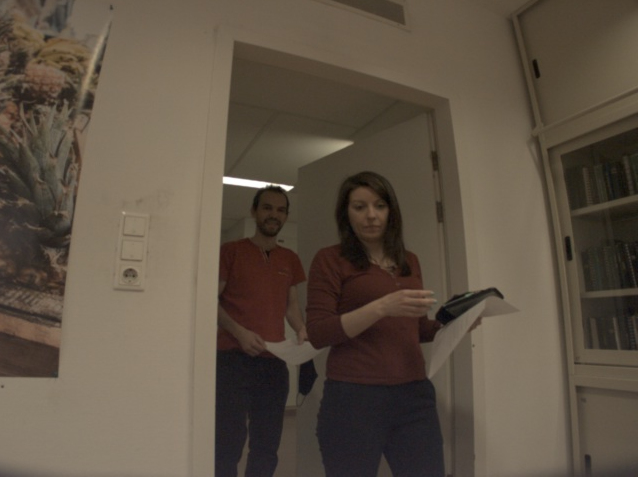
\includegraphics[width=\linewidth]{figures/video_examples/video_example_door.png}
    \end{subfigure}
    \begin{subfigure}[b]{0.45\linewidth}
        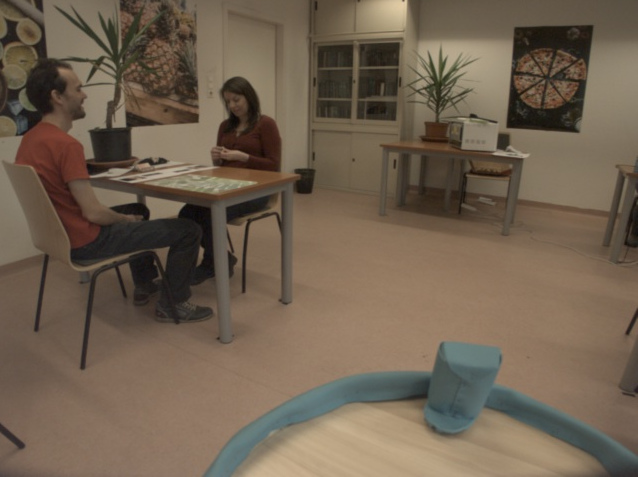
\includegraphics[width=\linewidth]{figures/video_examples/video_example_table_1.png}
    \end{subfigure}
    \begin{subfigure}[b]{0.45\linewidth}
        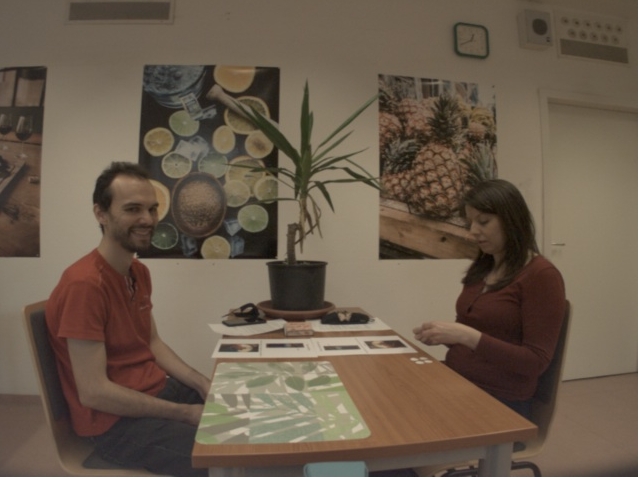
\includegraphics[width=\linewidth]{figures/video_examples/video_example_table_2.png}
    \end{subfigure}
    \begin{subfigure}[b]{0.45\linewidth}
        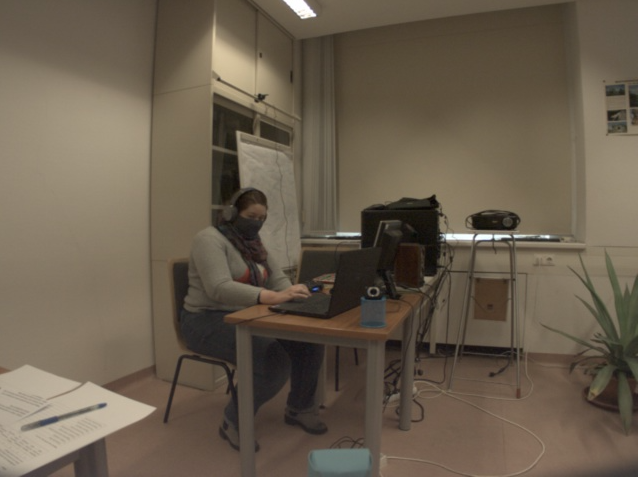
\includegraphics[width=\linewidth]{figures/video_examples/video_example_mask.png}
    \end{subfigure}
    \begin{subfigure}[b]{0.45\linewidth}
        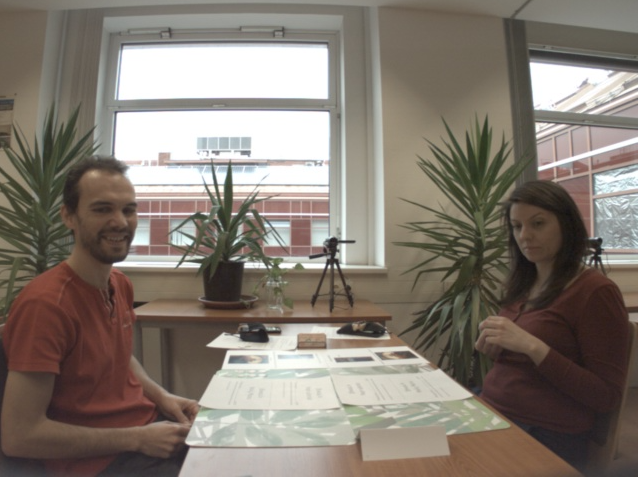
\includegraphics[width=\linewidth]{figures/video_examples/video_example_back_illumination.png}
    \end{subfigure}
    \begin{subfigure}[b]{0.45\linewidth}
        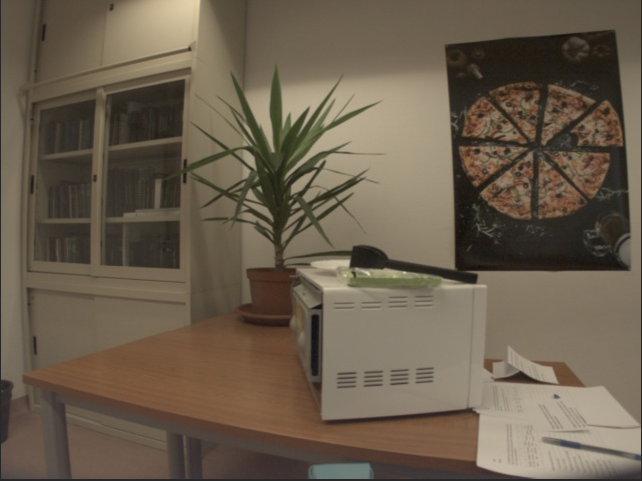
\includegraphics[width=\linewidth]{figures/video_examples/video_example_empty.png}
    \end{subfigure}
    \caption{Példák érdekes esetekre.}
    \label{fig:video_examples}
\end{figure}

\section{Az értékelések eredményei, a választott algoritmus}
A kiértékelést először a kisebb méretű adatszetteken hajtottam végre. Az eredmények a \ref{fig:afw_evaluation}-\ref{fig:fddb_evaluation}. ábrákon láthatóak. A kiértékelést ezeken a faceboxes készítői által ajánlott kiértékelő kóddal végeztem. A kódot tartalmazó repository a készítők által mért korábbi eredményeket is tartalmazza, ezek közül párat megtartottam összehasonlításképp. Ezek alapján megállapítható, hogy a régebbi modellek pontossága jelentősen elmarad az újakéval szemben. A faceboxes és az insightface által nyújtott modellek eredményei azonban mind olyan magasak, és közel helyezkednek el, hogy ezek alapján nem hozható releváns döntés.
\begin{figure}
    \centering
    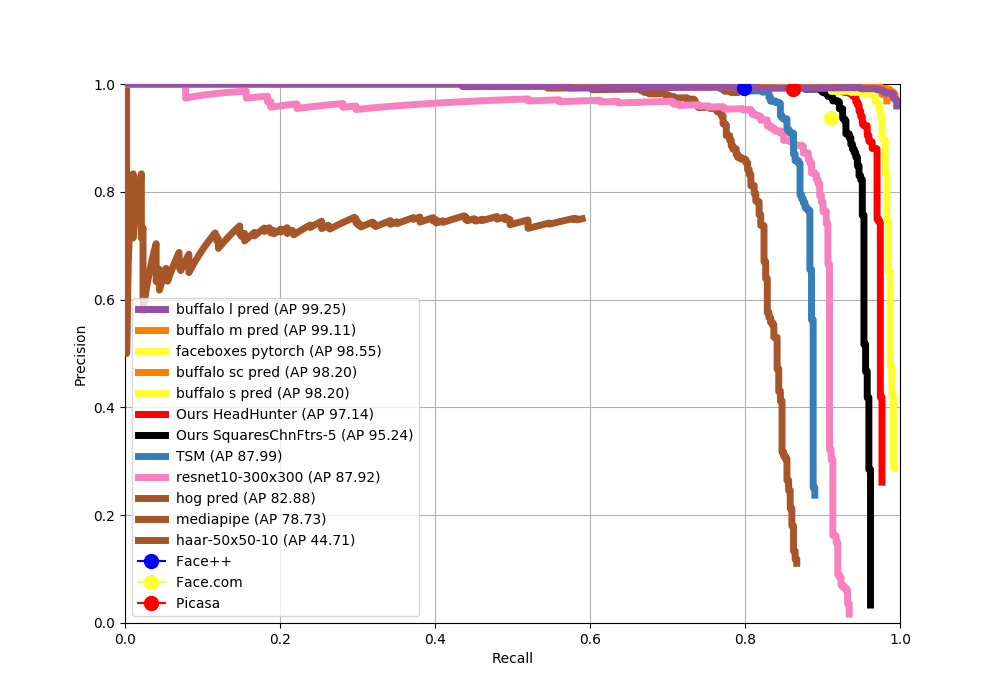
\includegraphics[width=\linewidth]{figures/afw.png}
    \caption{AFW}
    \label{fig:afw_evaluation}
\end{figure}
\begin{figure}
    \centering
    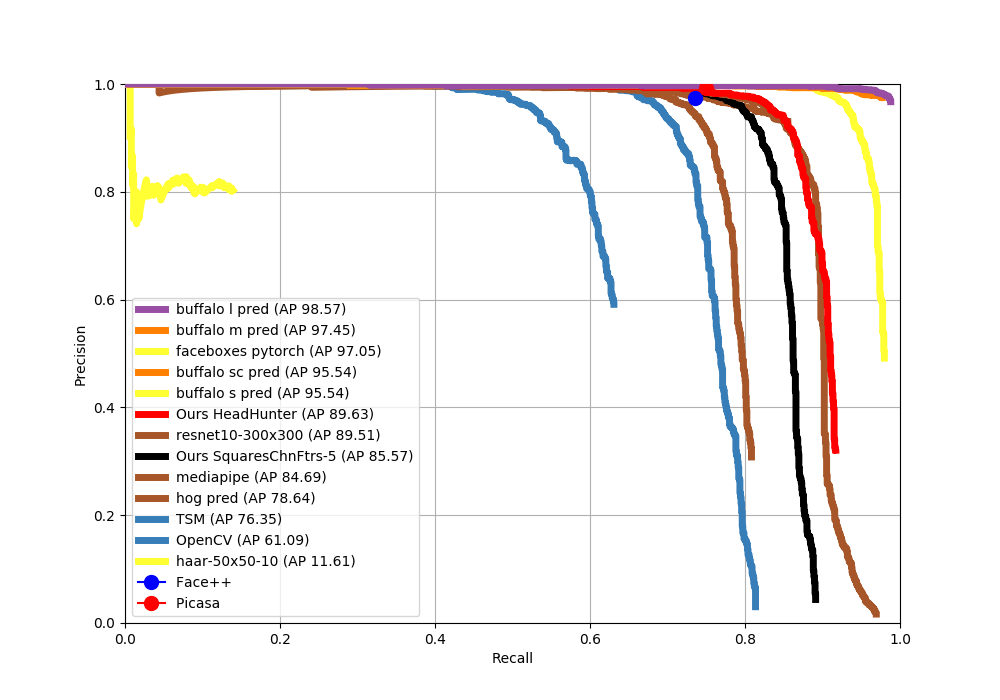
\includegraphics[width=\linewidth]{figures/pascal.png}
    \caption{PASCAL face}
    \label{fig:pascal_evaluation}
\end{figure}
\begin{figure}
    \centering
    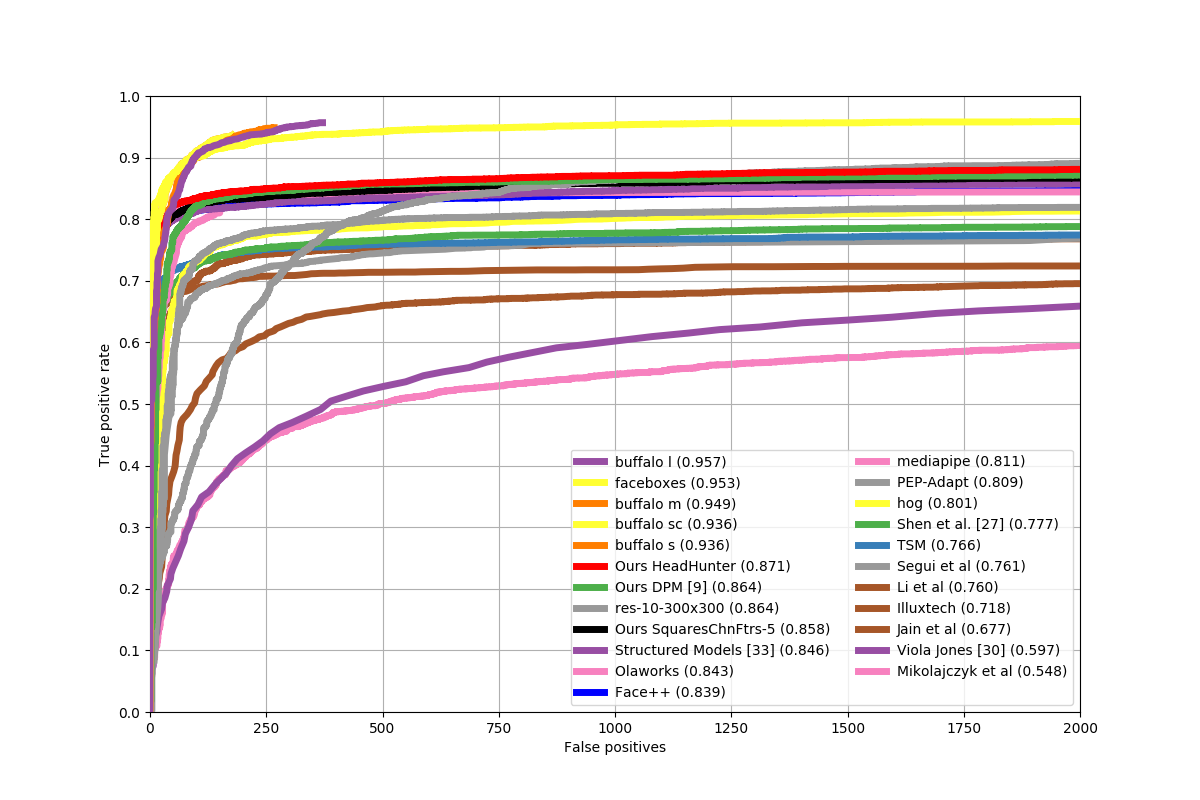
\includegraphics[width=\linewidth]{figures/fddb.png}
    \caption{FDDB}
    \label{fig:fddb_evaluation}
\end{figure}

A legjobb értékeket elért algoritmusokat ezért a WIDER adatszett validációs részén is teszteltem, melyhez hivatalos kiértékelő MATLAB kód tartozik. Érdekes eredmény, hogy míg a korábbi esetekben a faceboxes minden alkalommal a buffalo\_m modellhez hasonló eredményeket produkált, itt az összes insightface modellhez képest jelentősen rosszabb pontszámot ért el. Ez alapján kijelenthető, hogy amennyiben bármelyik buffalo modell gyorsabbnak bizonyul, érdemes lehet azt előnyben részesíteni, főleg mivel azokhoz API is társul, míg a faceboxes implementáció kezelése lényegesen körülményesebb.

\begin{figure}
    \centering
    \begin{subfigure}[b]{0.75\linewidth}
        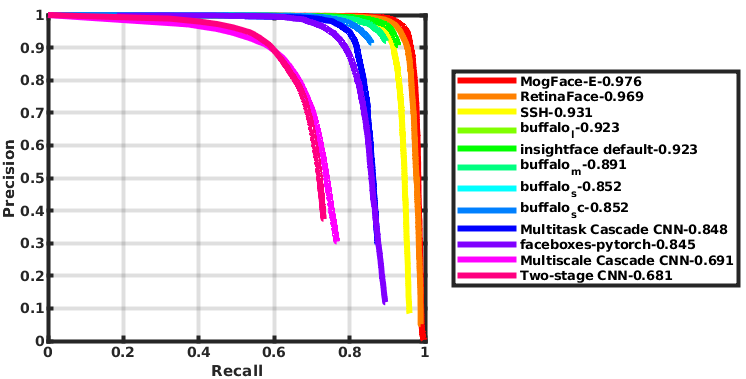
\includegraphics[width=\linewidth]{figures/wider_easy.png}
        \caption{Easy}
    \end{subfigure}
    \begin{subfigure}[b]{0.75\linewidth}
        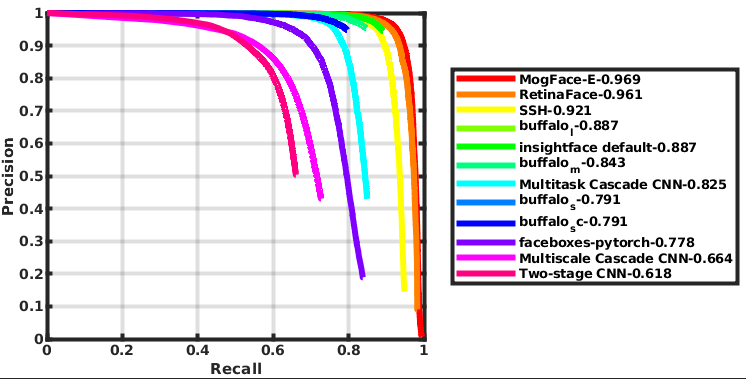
\includegraphics[width=\linewidth]{figures/wider_medium.png}
        \caption{Medium}
    \end{subfigure}
    \begin{subfigure}[b]{0.75\linewidth}
        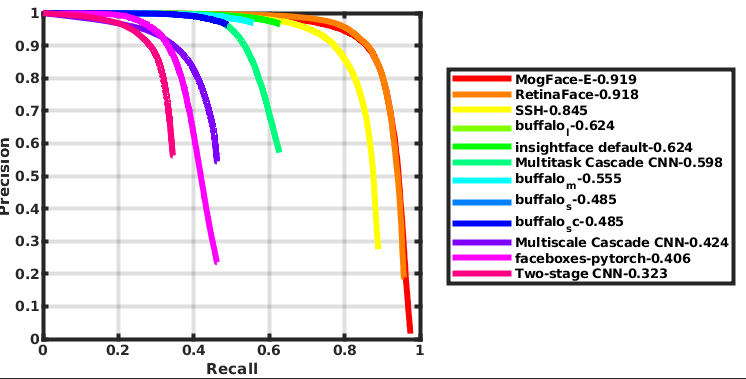
\includegraphics[width=\linewidth]{figures/wider_hard.png}
        \caption{Hard}
    \end{subfigure}
    \caption{A WIDER adatszetten mért eredmények.}
    \label{fig:wider_evaluation}
\end{figure}

\section{ROS node kialakítása}
%%----------------------------------------------------------------------------
\chapter{\LaTeX-eszközök}
\label{sec:LatexTools}
%----------------------------------------------------------------------------
\section{A szerkesztéshez használatos eszközök}
%----------------------------------------------------------------------------

Ez a sablon TeXstudio 2.8.8 szerkesztővel készült. A TeXstudio egy platformfüggetlen, Windows, Linux és Mac OS alatt is elérhető \LaTeX-szerkesztőprogram számtalan hasznos szolgáltatással (\refstruc{fig:TeXstudio}). A szoftver ingyenesen letölthető\footnote{A TeXstudio hivatalos oldala: \url{http://texstudio.sourceforge.net/}}.

\begin{figure}[!ht]
    \centering
    \includegraphics[width=150mm, keepaspectratio]{figures/TeXstudio.png}
    \caption{A TeXstudio \LaTeX-szerkesztő.}
    \label{fig:TeXstudio}
\end{figure}

A TeXstudio telepítése után érdemes még letölteni a magyar nyelvű helyesírásellenőrző-szótárakat hozzá. A TeXstudio az OpenOffice-hoz használatos formátumot tudja kezelni. A TeXstudio beállításainál a \verb+General+ fülön a \verb+Dictionaries+ résznél tudjuk megadni, hogy melyik szótárat használja.

Egy másik használható Windows alapú szerkesztőprogram a LEd\footnote{A LEd hivatalos oldala: \url{http://www.latexeditor.org/}} (LaTeX Editor), a TeXstudio azonban stabilabb, gyorsabb, és jobban használható.

%----------------------------------------------------------------------------
\section{A dokumentum lefordítása Windows alatt}
%----------------------------------------------------------------------------
A TeXstudio és a LEd kizárólag szerkesztőprogram (bár az utóbbiban DVI-nézegető is van), így a dokumentum fordításához szükséges eszközöket nem tartalmazza. Windows alatt alapvetően két lehetőség közül érdemes választani: MiKTeX (\url{http://miktex.org/}) és TeX Live (\url{http://www.tug.org/texlive/}) programcsomag. Az utóbbi működik Mac OS X, GNU/Linux alatt és Unix-származékokon is. A MiKTeX egy alapcsomag telepítése után mindig letölti a használt funkciókhoz szükséges, de lokálisan hiányzó \TeX-csomagokat, míg a TeX Live DVD ISO verzóban férhető hozzá. Ez a dokumentum TeX Live 2008 programcsomag segítségével fordult, amelynek DVD ISO verziója a megadott oldalról letölthető. A sablon lefordításához a disztribúcióban szereplő \verb+magyar.ldf+ fájlt a \verb+http://www.math.bme.hu/latex/+ változatra kell cserélni, vagy az utóbbi változatot be kell másolni a projekt-könyvtárba (ahogy ezt meg is tettük a sablonban) különben anomáliák tapasztalhatók a dokumentumban (pl. az ábra- és táblázat-aláírások formátuma nem a beállított lesz, vagy bizonyos oldalakon megjelenik alapértelmezésben egy fejléc). A TeX Live 2008-at még nem kell külön telepíteni a gépre, elegendő DVD-ről (vagy az ISO fájlból közvetlenül, pl. DaemonTools-szal) használni.

Ha a MiKTeX csomagot használjuk, akkor parancssorból a következő módon tudjuk újrafordítani a teljes dokumentumot:

\begin{lstlisting}[language=bash,frame=single,float=!ht]
$ texify -p thesis.tex
\end{lstlisting}

A \verb+texify+ parancs a MiKTex programcsomag \verb+miktex/bin+ alkönyvtárában található. A parancs gondoskodik arról, hogy a szükséges lépéseket (fordítás, hivatkozások generálása stb.) a megfelelő sorrendben elvégezze. A \verb+-p+ kapcsoló hatására PDF-et generál. A fordítást és az ideiglenes fájlok törlését elvégezhetjük a sablonhoz mellékelt \verb+manual_build.bat+ szkript segítségével is.

A \TeX-eszközöket tartalmazó programcsomag binárisainak elérési útját gyakran be kell állítani a szerkesztőprogramban, például TeXstudio esetén legegyszerűbben az \verb+Options / Configure TeXstudio... / Commands+ menüponttal előhívott dialógusablakban tehetjük ezt meg.

A PDF-\LaTeX~használata esetén a generált dokumentum közvetlenül PDF-formátumban áll rendelkezésre. Amennyiben a PDF-fájl egy PDF-nézőben (pl. Adobe Acrobat Reader vagy Foxit PDF Reader) meg van nyitva, akkor a fájlleírót a PDF-néző program tipikusan lefoglalja. Ilyen esetben a dokumentum újrafordítása hibaüzenettel kilép. Ha bezárjuk és újra megnyitjuk a PDF dokumentumot, akkor pedig a PDF-nézők többsége az első oldalon nyitja meg a dokumentumot, nem a legutóbb olvasott oldalon. Ezzel szemben például az egyszerű és ingyenes \textcolor{blue}{Sumatra PDF} nevű program képes arra, hogy a megnyitott dokumentum megváltozását detektálja, és frissítse a nézetet az aktuális oldal megtartásával.

%----------------------------------------------------------------------------
\section{Eszközök Linuxhoz}
%----------------------------------------------------------------------------
Linux operációs rendszer alatt is rengeteg szerkesztőprogram van, pl. a KDE alapú Kile jól használható. Ez ingyenesen letölthető, vagy éppenséggel az adott Linux-disztribúció eleve tartalmazza, ahogyan a dokumentum fordításához szükséges csomagokat is. Az Ubuntu Linux disztribúciók alatt például legtöbbször a \verb+texlive-*+ csomagok telepítésével használhatók a \LaTeX-eszközök. A jelen sablon fordításához szükséges csomagok (kb. 0,5 GB) az alábbi paranccsal telepíthetők:

\begin{lstlisting}[language=bash,morekeywords={sudo,apt\-get},alsoletter={-},breaklines=true]
$ sudo apt-get install texlive-latex-extra texlive-fonts-extra texlive-fonts-recommended texlive-xetex texlive-science texlive-lang-european
\end{lstlisting}

Amennyiben egy újabb csomag hozzáadása után hiányzó fájlra utaló hibát kapunk a fordítótól, telepítenünk kell az azt tartalmazó TeX Live csomagot. Ha pl. a \verb+bibentry+ csomagot szeretnénk használni, futtassuk az alábbi parancsot:

\begin{lstlisting}[language=bash,morekeywords={apt\-cache},alsoletter={-},breaklines=true]
$ apt-cache search bibentry
texlive-luatex - TeX Live: LuaTeX packages
\end{lstlisting}

Majd telepítsük fel a megfelelő TeX Live csomagot, jelen esetben a `texlive-lualatex`-et. (Egy LaTeX csomag több TeX Live csomagban is szerepelhet.)

Ha gyakran szerkesztünk más \LaTeX dokumentumokat is, kényelmes és biztos megoldás a teljes TeX Live disztribúció telepítése, ez azonban kb. 4 GB helyet igényel.

\begin{lstlisting}[language=bash,morekeywords={sudo,apt\-get},alsoletter={-},breaklines=true]
sudo apt-get install texlive-full
\end{lstlisting}
       % 2. fejezet
%%----------------------------------------------------------------------------
\chapter{A dolgozat formai kivitele}
%----------------------------------------------------------------------------
Az itt található információk egy része a BME VIK Hallgatói Képviselet által készített ,,Utolsó félév a villanykaron'' c. munkából lett kis változtatásokkal átemelve. Az eredeti dokumentum az alábbi linken érhető el: \url{http://vik.hk/hirek/diplomafelev-howto-2015}.

%----------------------------------------------------------------------------
\section{A dolgozat kimérete}
%----------------------------------------------------------------------------
Szakdolgozat esetében minimum 30, 45 körüli ajánlott oldalszám lehet az iránymutató. De mindenképp érdemes rákérdezni a konzulensnél is az elvárásokra, mert tanszékenként változóak lehetnek az elvárások.

Mesterképzésen a Diplomatervezés 1 esetében a beszámoló még inkább az Önálló laboratóriumi beszámolókhoz hasonlít, tanszékenként eltérő formai követelményekkel, -- egy legalább 30 oldal körüli dolgozat az elvárt -- és az elmúlt fél éves munkáról szól. De egyben célszerű, ha ez a végleges diplomaterv alapja is. (A végleges 60-90 oldal körülbelül a hasznos részre nézve)


%----------------------------------------------------------------------------
\section{A dolgozat nyelve}
%----------------------------------------------------------------------------
Mivel Magyarországon a hivatalos nyelv a magyar, ezért alapértelmezésben magyarul kell megírni a dolgozatot. Aki külföldi posztgraduális képzésben akar részt venni, nemzetközi szintű tudományos kutatást szeretne végezni, vagy multinacionális cégnél akar elhelyezkedni, annak célszerű angolul megírnia diplomadolgozatát. Mielőtt a hallgató az angol nyelvű verzió mellett dönt, erősen ajánlott mérlegelni, hogy ez mennyi többletmunkát fog a hallgatónak jelenteni fogalmazás és nyelvhelyesség terén, valamint -- nem utolsó sorban -- hogy ez mennyi többletmunkát fog jelenteni a konzulens illetve bíráló számára. Egy nehezen olvasható, netalán érthetetlen szöveg teher minden játékos számára.

%----------------------------------------------------------------------------
\section{A dokumentum nyomdatechnikai kivitele}
%----------------------------------------------------------------------------
A dolgozatot A4-es fehér lapra nyomtatva, 2,5 centiméteres margóval (+1~cm kötésbeni), 11--12 pontos betűmérettel, talpas betűtípussal és másfeles sorközzel célszerű elkészíteni.

Annak érdekében, hogy a dolgozat külsőleg is igényes munka benyomását keltse, érdemes figyelni az alapvető tipográfiai szabályok betartására~\cite{Jeney}.
     % 3. fejezet
%%----------------------------------------------------------------------------
\chapter{A \LaTeX-sablon használata}
%----------------------------------------------------------------------------

Ebben a fejezetben röviden, implicit módon bemutatjuk a sablon használatának módját, ami azt jelenti, hogy sablon használata ennek a dokumentumnak a forráskódját tanulmányozva válik teljesen világossá. Amennyiben a szoftver-keretrendszer telepítve van, a sablon alkalmazása és a dolgozat szerkesztése \LaTeX-ben a sablon segítségével tapasztalataink szerint jóval hatékonyabb, mint egy WYSWYG (\emph{What You See is What You Get}) típusú szövegszerkesztő esetén (pl. Microsoft Word, OpenOffice).

%----------------------------------------------------------------------------
\section{Címkék és hivatkozások}
%----------------------------------------------------------------------------
A \LaTeX~dokumentumban címkéket (\verb+\label+) rendelhetünk ábrákhoz, táblázatokhoz, fejezetekhez, listákhoz, képletekhez stb. Ezekre a dokumentum bármely részében hivatkozhatunk, a hivatkozások automatikusan feloldásra kerülnek.

A sablonban makrókat definiáltunk a hivatkozások megkönnyítéséhez. Ennek megfelelően minden ábra (\emph{figure}) címkéje \verb+fig:+ kulcsszóval kezdődik, míg minden táblázat (\emph{table}), képlet (\emph{equation}), fejezet (\emph{section}) és lista (\emph{listing}) rendre a \verb+tab:+, \verb+eq:+, \verb+sec:+ és \verb+lst:+ kulcsszóval kezdődik, és a kulcsszavak után tetszőlegesen választott címke használható. Ha ezt a konvenciót betartjuk, akkor az előbbi objektumok számára rendre a \verb+\figref+, \verb+\tabref+, \verb+\eqref+, \verb+\sectref+ és \verb+\listref+ makrókkal hivatkozhatunk. A makrók paramétere a címke, amelyre hivatkozunk (a kulcsszó nélkül). Az összes említett hivatkozástípus, beleértve az \verb+\url+ kulcsszóval bevezetett web-hivatkozásokat is a  \verb+hyperref+\footnote{Segítségével a dokumentumban megjelenő hivatkozások nem csak dinamikussá válnak, de színezhetők is, bővebbet erről a csomag dokumentációjában találunk. Ez egyúttal egy példa lábjegyzet írására.} csomagnak köszönhetően aktívak a legtöbb PDF-nézegetőben, rájuk kattintva a dokumentum megfelelő oldalára ugrik a PDF-néző vagy a megfelelő linket megnyitja az alapértelmezett böngészővel. A \verb+hyperref+ csomag a kimeneti PDF-dokumentumba könyvjelzőket is készít a tartalomjegyzékből. Ez egy szintén aktív tartalomjegyzék, amelynek elemeire kattintva a nézegető behozza a kiválasztott fejezetet.

%----------------------------------------------------------------------------
\section{Ábrák és táblázatok}
%----------------------------------------------------------------------------
Használjunk vektorgrafikus ábrákat, ha van rá módunk. PDFLaTeX használata esetén PDF formátumú ábrákat lehet beilleszteni könnyen, az EPS (PostScript) vektorgrafikus képformátum beillesztését a PDFLaTeX közvetlenül nem támogatja (de lehet konvertálni, lásd később). Ha vektorgrafikus formában nem áll rendelkezésünkre az ábra, akkor a  veszteségmentes PNG, valamint a veszteséges JPEG formátumban érdemes elmenteni.  Figyeljünk arra, hogy ilyenkor a képek felbontása elég nagy legyen ahhoz, hogy nyomtatásban is megfelelő minőséget nyújtson (legalább 300 dpi javasolt). A dokumentumban felhasznált képfájlokat a dokumentum forrása mellett érdemes tartani, archiválni, mivel ezek hiányában a dokumentum nem fordul újra. Ha lehet, a vektorgrafikus képeket vektorgrafikus formátumban is érdemes elmenteni az újrafelhasználhatóság (az átszerkeszthetőség) érdekében.

Kapcsolási rajzok legtöbbször kimásolhatók egy vektorgrafikus programba (pl. CorelDraw) és onnan nagyobb felbontással raszterizálva kimenthatők PNG formátumban. Ugyanakkor kiváló ábrák készíthetők Microsoft Visio vagy hasonló program használatával is: Visio-ból az ábrák közvetlenül PDF-be is menthetők.

Lehetőségeink Matlab ábrák esetén:
\begin{itemize}
	\item Képernyőlopás (\emph{screenshot}) is elfogadható minőségű lehet a dokumentumban, de általában jobb felbontást is el lehet érni más módszerrel.
	\item A Matlab ábrát a \verb+File/Save As+ opcióval lementhetjük PNG formátumban (ugyanaz itt is érvényes, mint korábban, ezért nem javasoljuk).
	\item A Matlab ábrát az \verb+Edit/Copy figure+ opcióval kimásolhatjuk egy vektorgrafikus programba is és onnan nagyobb felbontással raszterizálva kimenthatjük PNG formátumban (nem javasolt).
	\item Javasolt megoldás: az ábrát a \verb+File/Save As+ opcióval EPS \emph{vektorgrafikus} formátumban elmentjük, PDF-be konvertálva beillesztjük a dolgozatba.
\end{itemize}
Az EPS kép az \verb+epstopdf+ programmal\footnote{a korábban említett \LaTeX-disztribúciókban megtalálható} konvertálható PDF formátumba. Célszerű egy batch-fájlt készíteni az összes EPS ábra lefordítására az alábbi módon (ez Windows alatt működik).
\begin{lstlisting}[language=]
@echo off
for %%j in (*.eps) do (
  echo converting file "%%j"
  epstopdf "%%j"
)
echo done .
\end{lstlisting}

Egy ilyen parancsfájlt (\verb+convert.cmd+) elhelyeztük a sablon \verb+figures\eps+ könyvtárába, így a felhasználónak csak annyi a dolga, hogy a \verb+figures\eps+ könyvtárba kimenti az EPS formátumú vektorgrafikus képet, majd lefuttatja a \verb+convert.cmd+ parancsfájlt, ami PDF-be konvertálja az EPS fájlt.

Ezek után a PDF-ábrát ugyanúgy lehet a dokumentumba beilleszteni, mint a PNG-t vagy a JPEG-et. A megoldás előnye, hogy a lefordított dokumentumban is vektorgrafikusan tárolódik az ábra, így a mérete jóval kisebb, mintha raszterizáltuk volna beillesztés előtt. Ez a módszer minden -- az EPS formátumot ismerő -- vektorgrafikus program (pl. CorelDraw) esetén is használható.

A képek beillesztésére \az+\refstruc{sec:LatexTools}ben mutattunk be példát (\refstruc{fig:TeXstudio}). Az előző mondatban egyúttal az automatikusan feloldódó ábrahivatkozásra is láthatunk példát. Több képfájlt is beilleszthetünk egyetlen ábrába. Az egyes képek közötti horizontális és vertikális margót metrikusan szabályozhatjuk (\refstruc{fig:HVSpaces}). Az ábrák elhelyezését számtalan tipográfiai szabály egyidejű teljesítésével a fordító maga végzi, a dokumentum írója csak preferenciáit jelezheti a fordító felé (olykor ez bosszúságot is okozhat, ilyenkor pl. a kép méretével lehet játszani).

\begin{figure}[!ht]
	\centering
	\includegraphics[width=67mm, keepaspectratio]{figures/TeXstudio.png}\hspace{1cm}
	\includegraphics[width=67mm, keepaspectratio]{figures/TeXstudio.png}\\\vspace{5mm}
	\includegraphics[width=67mm, keepaspectratio]{figures/TeXstudio.png}\hspace{1cm}
	\includegraphics[width=67mm, keepaspectratio]{figures/TeXstudio.png}
	\caption{Több képfájl beillesztése esetén térközöket is érdemes használni.}
	\label{fig:HVSpaces}
\end{figure}

A táblázatok használatára \aref{tab:TabularExample}~táblázat mutat példát. A táblázatok formázásához hasznos tanácsokat találunk a \verb+booktabs+ csomag dokumentációjában.

\begin{table}[!ht]
	\footnotesize
	\centering
	\begin{tabular}{ l c c }
		\toprule
		Órajel & Frekvencia & Cél pin \\
		\midrule
		CLKA & 100 MHz & FPGA CLK0\\
		CLKB & 48 MHz  & FPGA CLK1\\
		CLKC & 20 MHz  & Processzor\\
		CLKD & 25 MHz  & Ethernet chip \\
		CLKE & 72 MHz  & FPGA CLK2\\
		XBUF & 20 MHz  & FPGA CLK3\\
		\bottomrule
	\end{tabular}
	\caption{Az órajel-generátor chip órajel-kimenetei.}
	\label{tab:TabularExample}
\end{table}


%----------------------------------------------------------------------------
\section{Felsorolások és listák}
%----------------------------------------------------------------------------
Számozatlan felsorolásra mutat példát a jelenlegi bekezdés:
\begin{itemize}
	\item \emph{első bajusz:} ide lehetne írni az első elem kifejését,
	\item \emph{második bajusz:} ide lehetne írni a második elem kifejését,
	\item \emph{ez meg egy szakáll:} ide lehetne írni a harmadik elem kifejését.
\end{itemize}

Számozott felsorolást is készíthetünk az alábbi módon:
\begin{enumerate}
	\item \emph{első bajusz:} ide lehetne írni az első elem kifejését, és ez a kifejtés így néz ki, ha több sorosra sikeredik,
	\item \emph{második bajusz:} ide lehetne írni a második elem kifejését,
	\item \emph{ez meg egy szakáll:} ide lehetne írni a harmadik elem kifejését.
\end{enumerate}
A felsorolásokban sorok végén vessző, az utolsó sor végén pedig pont a szokásos írásjel. Ez alól kivételt képezhet, ha az egyes elemek több teljes mondatot tartalmaznak.

Listákban a dolgozat szövegétől elkülönítendő kódrészleteket, programsorokat, pszeudo-kódokat jeleníthetünk meg (\ref{lst:Example}.~kódrészlet).
\begin{lstlisting}[language=tex,caption=A fenti számozott felsorolás \LaTeX-forráskódja,label=lst:Example]
\begin{enumerate}
	\item \emph{els(*@ő@*) bajusz:} ide lehetne írni az els(*@ő@*) elem kifejését,
	és ez a kifejtés így néz ki, ha több sorosra sikeredik,
	\item \emph{második bajusz:} ide lehetne írni a második elem kifejését,
	\item \emph{ez meg egy szakáll:} ide lehetne írni a harmadik elem kifejését.
\end{enumerate}
\end{lstlisting}
A lista keretét, háttérszínét, egész stílusát megválaszthatjuk. Ráadásul különféle programnyelveket és a nyelveken belül kulcsszavakat is definiálhatunk, ha szükséges. Erről bővebbet a \verb+listings+ csomag hivatalos leírásában találhatunk.

%----------------------------------------------------------------------------
\section{Képletek}
%----------------------------------------------------------------------------
Ha egy formula nem túlságosan hosszú, és nem akarjuk hivatkozni a szövegből, mint például a $e^{i\pi}+1=0$ képlet, \emph{szövegközi képletként} szokás leírni. Csak, hogy másik példát is lássunk, az $U_i=-d\Phi/dt$ Faraday-törvény a $\rot E=-\frac{dB}{dt}$ differenciális alakban adott Maxwell-egyenlet felületre vett integráljából vezethető le. Látható, hogy a \LaTeX-fordító a sorközöket betartja, így a szöveg szedése esztétikus marad szövegközi képletek használata esetén is.

Képletek esetén az általános konvenció, hogy a kisbetűk skalárt, a kis félkövér betűk ($\mathbf{v}$) oszlopvektort -- és ennek megfelelően $\mathbf{v}^T$ sorvektort -- a kapitális félkövér betűk ($\mathbf{V}$) mátrixot jelölnek. Ha ettől el szeretnénk térni, akkor az alkalmazni kívánt jelölésmódot célszerű külön alfejezetben definiálni. Ennek megfelelően, amennyiben $\mathbf{y}$ jelöli a mérések vektorát, $\mathbf{\vartheta}$ a paraméterek vektorát és $\hat{\mathbf{y}}=\mathbf{X}\vartheta$ a paraméterekben lineáris modellt, akkor a \emph{Least-Squares} értelemben optimális paraméterbecslő $\hat{\mathbf{\vartheta}}_{LS}=(\mathbf{X}^T\mathbf{X})^{-1}\mathbf{X}^T\mathbf{y}$ lesz.

Emellett kiemelt, sorszámozott képleteket is megadhatunk, ennél az \verb+equation+ és a \verb+eqnarray+ környezetek helyett a korszerűbb \verb+align+ környezet alkalmazását javasoljuk (több okból, különféle problémák elkerülése végett, amelyekre most nem térünk ki). Tehát
\begin{align}
\dot{\mathbf{x}}&=\mathbf{A}\mathbf{x}+\mathbf{B}\mathbf{u},\\
\mathbf{y}&=\mathbf{C}\mathbf{x},
\end{align}
ahol $\mathbf{x}$ az állapotvektor, $\mathbf{y}$ a mérések vektora és $\mathbf{A}$, $\mathbf{B}$ és $\mathbf{C}$ a rendszert leíró paramétermátrixok. Figyeljük meg, hogy a két egyenletben az egyenlőségjelek egymáshoz igazítva jelennek meg, mivel a mindkettőt az \& karakter előzi meg a kódban. Lehetőség van számozatlan kiemelt képlet használatára is, például
\begin{align}
\dot{\mathbf{x}}&=\mathbf{A}\mathbf{x}+\mathbf{B}\mathbf{u},\nonumber\\
\mathbf{y}&=\mathbf{C}\mathbf{x}\nonumber.
\end{align}
Mátrixok felírására az $\mathbf{A}\mathbf{x}=\mathbf{b}$ inhomogén lineáris egyenlet részletes kifejtésével mutatunk példát:
\begin{align}
\begin{bmatrix}
a_{11} & a_{12} & \dots & a_{1n}\\
a_{21} & a_{22} & \dots & a_{2n}\\
\vdots & \vdots & \ddots & \vdots\\
a_{m1} & a_{m2} & \dots & a_{mn}
\end{bmatrix}
\begin{pmatrix}x_1\\x_2\\\vdots\\x_n\end{pmatrix}=
\begin{pmatrix}b_1\\b_2\\\vdots\\b_m\end{pmatrix}.
\end{align}
A \verb+\frac+ utasítás hatékonyságát egy általános másodfokú tag átviteli függvényén keresztül mutatjuk be, azaz
\begin{align}
W(s)=\frac{A}{1+2T\xi s+s^2T^2}.
\end{align}
A matematikai mód minden szimbólumának és képességének a bemutatására természetesen itt nincs lehetőség, de gyors referenciaként hatékonyan használhatók a következő linkek:\\
\indent\url{http://www.artofproblemsolving.com/LaTeX/AoPS_L_GuideSym.php},\\
\indent\url{http://www.ctan.org/tex-archive/info/symbols/comprehensive/symbols-a4.pdf},\\
\indent\url{ftp://ftp.ams.org/pub/tex/doc/amsmath/short-math-guide.pdf}.\\
Ez pedig itt egy magyarázat, hogy miért érdemes \verb+align+ környezetet használni:\\
\indent\url{http://texblog.net/latex-archive/maths/eqnarray-align-environment/}.

%----------------------------------------------------------------------------
\section{Irodalmi hivatkozások}
\label{sec:HowtoReference}
%----------------------------------------------------------------------------
Egy \LaTeX~dokumentumban az irodalmi hivatkozások definíciójának két módja van. Az egyik a \verb+\thebibliograhy+ környezet használata a dokumentum végén, az \verb+\end{document}+ lezárás előtt.
\begin{lstlisting}[language=tex]
\begin{thebibliography}{9}

\bibitem{Lamport94} Leslie Lamport, \emph{\LaTeX: A Document Preparation System}.
Addison Wesley, Massachusetts, 2nd Edition, 1994.

\end{thebibliography}
\end{lstlisting}

Ezek után a dokumentumban a \verb+\cite{Lamport94}+ utasítással hivatkozhatunk a forrásra. A fenti megadás viszonylag kötetlen, a szerző maga formázza az irodalomjegyzéket (ami gyakran inkonzisztens eredményhez vezet).

Egy sokkal professzionálisabb módszer a BiB\TeX{} használata, ezért ez a sablon is ezt támogatja. Ebben az esetben egy külön szöveges adatbázisban definiáljuk a forrásmunkákat, és egy külön stílusfájl határozza meg az irodalomjegyzék kinézetét. Ez, összhangban azzal, hogy külön formátumkonvenció határozza meg a folyóirat-, a könyv-, a konferenciacikk- stb. hivatkozások kinézetét az irodalomjegyzékben (a sablon használata esetén ezzel nem is kell foglalkoznia a hallgatónak, de az eredményt célszerű ellenőrizni). felhasznált hivatkozások adatbázisa egy \verb+.bib+ kiterjesztésű szöveges fájl, amelynek szerkezetét a \Aref{lst:Bibtex} kódrészlet demonstrálja. A forrásmunkák bevitelekor a sor végi vesszők külön figyelmet igényelnek, mert hiányuk a BiB\TeX-fordító hibaüzenetét eredményezi. A forrásmunkákat típus szerinti kulcsszó vezeti be (\verb+@book+ könyv, \verb+@inproceedings+ konferenciakiadványban megjelent cikk, \verb+@article+ folyóiratban megjelent cikk, \verb+@techreport+ valamelyik egyetem gondozásában megjelent műszaki tanulmány, \verb+@manual+ műszaki dokumentáció esetén stb.). Nemcsak a megjelenés stílusa, de a kötelezően megadandó mezők is típusról-típusra változnak. Egy jól használható referencia a \url{http://en.wikipedia.org/wiki/BibTeX} oldalon található.

\begin{lstlisting}[caption=Példa szöveges irodalomjegyzék-adatbázisra Bib\TeX{} használata esetén.,label=lst:Bibtex]
@book{Wettl04,
  author    = {Ferenc Wettl and Gyula Mayer and Péter Szabó},
  publisher = {Panem Könyvkiadó},
  title     = {\LaTeX~kézikönyv},
  year      = {2004},
}

@article{Candy86,
  author       = {James C. Candy},
  journaltitle = {{IEEE} Trans.\ on Communications},
  month        = {01},
  note         = {\doi{10.1109/TCOM.1986.1096432}},
  number       = {1},
  pages        = {72--76},
  title        = {Decimation for Sigma Delta Modulation},
  volume       = {34},
  year         = {1986},
}

@inproceedings{Lee87,
  author    = {Wai L. Lee and Charles G. Sodini},
  booktitle = {Proc.\ of the IEEE International Symposium on Circuits and Systems},
  location  = {Philadelphia, PA, USA},
  month     = {05~4--7},
  pages     = {459--462},
  title     = {A Topology for Higher Order Interpolative Coders},
  vol       = {2},
  year      = {1987},
}

@thesis{KissPhD,
  author      = {Peter Kiss},
  institution = {Technical University of Timi\c{s}oara, Romania},
  month       = {04},
  title       = {Adaptive Digital Compensation of Analog Circuit Imperfections for Cascaded Delta-Sigma Analog-to-Digital Converters},
  type        = {phdthesis},
  year        = {2000},
}

@manual{Schreier00,
  author       = {Richard Schreier},
  month        = {01},
  note         = {\url{http://www.mathworks.com/matlabcentral/fileexchange/}},
  organization = {Oregon State University},
  title        = {The Delta-Sigma Toolbox v5.2},
  year         = {2000},
}

@misc{DipPortal,
  author       = {{Budapesti Műszaki és Gazdaságtudományi Egyetem Villamosmérnöki és Informatikai Kar}},
  howpublished = {\url{http://diplomaterv.vik.bme.hu/}},
  title        = {Diplomaterv portál (2011. február 26.)},
}

@incollection{Mkrtychev:1997,
  author    = {Mkrtychev, Alexey},
  booktitle = {Logical Foundations of Computer Science},
  doi       = {10.1007/3-540-63045-7_27},
  editor    = {Adian, Sergei and Nerode, Anil},
  isbn      = {978-3-540-63045-6},
  pages     = {266-275},
  publisher = {Springer Berlin Heidelberg},
  series    = {Lecture Notes in Computer Science},
  title     = {Models for the logic of proofs},
  url       = {http://dx.doi.org/10.1007/3-540-63045-7_27},
  volume    = {1234},
  year      = {1997},
}
\end{lstlisting}

A stílusfájl egy \verb+.sty+ kiterjesztésű fájl, de ezzel lényegében nem kell foglalkozni, mert vannak beépített stílusok, amelyek jól használhatók. Ez a sablon a BiB\TeX-et használja, a hozzá tartozó adatbázisfájl a \verb+mybib.bib+ fájl. Megfigyelhető, hogy az irodalomjegyzéket a dokumentum végére (a \verb+\end{document}+ utasítás elé) beillesztett \verb+\bibliography{mybib}+ utasítással hozhatjuk létre, a stílusát pedig ugyanitt a  \verb+\bibliographystyle{plain}+ utasítással adhatjuk meg. Ebben az esetben a \verb+plain+ előre definiált stílust használjuk (a sablonban is ezt állítottuk be). A \verb+plain+ stíluson kívül természetesen számtalan más előre definiált stílus is létezik. Mivel a \verb+.bib+ adatbázisban ezeket megadtuk, a BiB\TeX-fordító is meg tudja különböztetni a szerzőt a címtől és a kiadótól, és ez alapján automatikusan generálódik az irodalomjegyzék a stílusfájl által meghatározott stílusban.

Az egyes forrásmunkákra a szövegből továbbra is a \verb+\cite+ paranccsal tudunk hivatkozni, így \aref{lst:Bibtex}.~kódrészlet esetén a hivatkozások rendre \verb+\cite{Wettl04}+, \verb+\cite{Candy86}+, \verb+\cite{Lee87}+, \verb+\cite{KissPhD}+, \verb+\cite{Schreirer00}+,
\verb+\cite{Mkrtychev:1997}+ és \verb+\cite{DipPortal}+. Az egyes forrásmunkák sorszáma az irodalomjegyzék bővítésekor változhat. Amennyiben az aktuális számhoz illeszkedő névelőt szeretnénk használni, használjuk az \verb+\acite{}+ parancsot.

Az irodalomjegyzékben alapértelmezésben csak azok a forrásmunkák jelennek meg, amelyekre található hivatkozás a szövegben, és ez így alapvetően helyes is, hiszen olyan forrásmunkákat nem illik az irodalomjegyzékbe írni, amelyekre nincs hivatkozás.

Mivel a fordítási folyamat során több lépésben oldódnak fel a szimbólumok, ezért gyakran többször is le kell fordítani a dokumentumot. Ilyenkor ez első 1-2 fordítás esetleg szimbólum-feloldásra vonatkozó figyelmeztető üzenettel zárul. Ha hibaüzenettel zárul bármelyik fordítás, akkor nincs értelme megismételni, hanem a hibát kell megkeresni. A \verb+.bib+ fájl megváltoztatáskor sokszor nincs hatása a változtatásnak azonnal, mivel nem mindig fut újra a BibTeX fordító. Ezért célszerű a változtatás után azt manuálisan is lefuttatni (TeXstudio esetén \verb+Tools/Bibliography+).

Hogy a szövegbe ágyazott hivatkozások kinézetét demonstráljuk, itt most sorban meghivatkozzuk a \cite{Wettl04}, \cite{Candy86}, \cite{Lee87}, \cite{KissPhD}, \cite{Schreier00} és \acite{Mkrtychev:1997}\footnote{Informatikai témában gyakran hivatkozunk cikkeket a Springer LNCS valamely kötetéből, ez a hivatkozás erre mutat egy helyes példát.} forrásmunkát, valamint \acite{DipPortal} weboldalt.

Megjegyzendő, hogy az ékezetes magyar betűket is tartalmazó \verb+.bib+ fájl az \verb+inputenc+ csomaggal betöltött \verb+latin2+ betűkészlet miatt fordítható. Ugyanez a \verb+.bib+ fájl hibaüzenettel fordul egy olyan dokumentumban, ami nem tartalmazza a \verb+\usepackage[latin2]{inputenc}+ sort. Speciális igény esetén az irodalmi adatbázis általánosabb érvényűvé tehető, ha az ékezetes betűket speciális latex karakterekkel helyettesítjük a \verb+.bib+ fájlban, pl. á helyett \verb+\'{a}+-t vagy ő helyett \verb+\H{o}+-t írunk.

Irodalomhivatkozásokat célszerű először olyan szolgáltatásokban keresni, ahol jó minőségű bejegyzések találhatók (pl. ACM Digital Library,\footnote{\url{https://dl.acm.org/}} DBLP,\footnote{\url{http://dblp.uni-trier.de/}} IEEE Xplore,\footnote{\url{http://ieeexplore.ieee.org/}} SpringerLink\footnote{\url{https://link.springer.com/}}) és csak ezek után használni kevésbé válogatott forrásokat (pl. Google Scholar\footnote{\url{http://scholar.google.com/}}). A jó minőségű bejegyzéseket is érdemes megfelelően tisztítani.\footnote{\url{https://github.com/FTSRG/cheat-sheets/wiki/BibTeX-Fixing-entries-from-common-sources}} A sablon angol nyelvű változatában használt \texttt{plainnat} beállítás egyik sajátossága, hogy a cikkhez generált hivatkozás a cikk DOI-ját és URL-jét is tartalmazza, ami gyakran duplikátumhoz vezet -- érdemes tehát a DOI-kat tartalmazó URL mezőket törölni. 

%----------------------------------------------------------------------------
\section{A dolgozat szerkezete és a forrásfájlok}
%----------------------------------------------------------------------------
A diplomatervsablonban a TeX fájlok két alkönyvtárban helyezkednek el. Az \verb+include+ könyvtárban azok szerepelnek, amiket tipikusan nem kell szerkesztenünk, ezek a sablon részei (pl. címoldal). A \verb+content+ alkönyvtárban pedig a saját munkánkat helyezhetjük el. Itt érdemes az egyes fejezeteket külön \TeX{} állományokba rakni.

A diplomatervsablon (a kari irányelvek szerint) az alábbi fő fejezetekből áll:
\begin{enumerate}
	\item \emph{szennycímoldal, sorozatcímoldal és címoldal} (\verb+include/titlepage.tex+),
	\item \emph{copyrightoldal} (\verb+include/copyrightpage.tex+),
	\item \emph{feladatkiírás} (\verb+include/project.tex+) a dolgozat nyomtatott verzójában ennek a helyére kerül a tanszék által kiadott, a tanszékvezető által aláírt feladatkiírás, a dolgozat elektronikus verziójába pedig a feladatkiírás egyáltalán ne kerüljön bele, azt külön tölti fel a tanszék a diplomaterv-honlapra,
	\item \emph{nyilatkozatok} (\verb+include/declaration.tex+),
	\item \emph{tartalomjegyzék} (\verb+thesis.tex+),
	\item \emph{illusztrációk és táblázatok jegyzéke} (\verb+thesis.tex+) \verb+\listoffigures+ és \verb+\listoftables+ utasításokkal generálható. Csak szükség esetén használandó, nem ajánlott.
	\item \emph{előszó} (\verb+chapters/preface.tex+),
	\item \emph{jelölések jegyzéke} (\verb+chapters/symbols.tex+),
	\item \emph{bevezetés} (\verb+chapters/introduction.tex+) a feladat értelmezése, a tervezés célja, a feladat indokoltsága, a diplomaterv felépítésének rövid összefoglalása,
	\item sorszámmal ellátott \emph{fejezetek} (\verb+chapters/chapter#.tex+) a feladatkiírás pontosítása és részletes elemzése, előzmények (irodalomkutatás, hasonló alkotások), az ezekből levonható következtetések, a tervezés részletes leírása, a döntési lehetőségek értékelése és a választott megoldások indoklása, a megtervezett műszaki alkotás értékelése, kritikai elemzése, továbbfejlesztési lehetőségek,
	\item részletes és pontos \emph{irodalomjegyzék} (ez a sablon esetében automatikusan generálódik a \verb+thesis.tex+ fájlban elhelyezett \verb+\bibliography+ utasítás hatására, \az+\refstruc{sec:HowtoReference}ban leírtak szerint),
	\item \emph{summary} (\verb+chapters/summary-foreign.tex+) idegen nyelvű összefoglaló,
	\item \emph{függelékek} (\verb+chapters/appendices.tex+),
	\item \emph{mellékletek} (\verb+chapters/annexes.tex+).
\end{enumerate}

%----------------------------------------------------------------------------
\section{Alapadatok megadása}
%----------------------------------------------------------------------------
A diplomaterv alapadatait (cím, szerző, konzulens, konzulens titulusa) a \verb+thesis.tex+ fájlban lehet megadni.

%----------------------------------------------------------------------------
\section{Új fejezet írása}
%----------------------------------------------------------------------------
A főfejezetek külön \verb+content+ könyvtárban foglalnak helyet. A sablonhoz 3 fejezet készült. További főfejezeteket úgy hozhatunk létre, ha új \TeX~fájlt készítünk a fejezet számára, és a \verb+thesis.tex+ fájlban, a \verb+\include+ és \verb+\includeonly+ utasítások argumentumába felvesszük az új \verb+.tex+ fájl nevét.


%----------------------------------------------------------------------------
\section{Definíciók, tételek, példák}
%----------------------------------------------------------------------------

\begin{definition}[Fluxuskondenzátor térerőssége]
Lorem ipsum dolor sit amet, consectetur adipiscing elit, sed do eiusmod tempor incididunt ut labore et dolore magna aliqua. Ut enim ad minim veniam, quis nostrud exercitation ullamco laboris nisi ut aliquip ex ea commodo consequat.
\end{definition}

\begin{example}
Példa egy példára. Duis aute irure dolor in reprehenderit in voluptate velit esse cillum dolore eu fugiat nulla pariatur. Excepteur sint occaecat cupidatat non proident, sunt in culpa qui officia deserunt mollit anim id est laborum.
\end{example}

\begin{theorem}[Kovács tétele]
Duis aute irure dolor in reprehenderit in voluptate velit esse cillum dolore eu fugiat nulla pariatur. Excepteur sint occaecat cupidatat non proident, sunt in culpa qui officia deserunt mollit anim id est laborum.
\end{theorem}
    % 4. fejezet
%----------------------------------------------------------------------------
\chapter{\osszefoglalas} % (Eredmények értékelése)
%----------------------------------------------------------------------------           % Összefoglalás


% Bibliográfia [Bibliography]
\addcontentsline{toc}{chapter}{\bibname}
{
    \footnotesize  % Kisebb betűméret [Smaller font size]
    \bibliography{bib/Diploma}
}


% Idegen nyelvű (angol) összefoglaló [Foreign language summary]
%----------------------------------------------------------------------------
\chapter*{\summary}\addcontentsline{toc}{chapter}{\summary}
%----------------------------------------------------------------------------

\selectforeignlanguage % angol (magyar) nyelvi beállítások

Az elvégzett munka rövid, másfél oldalt meg nem haladó, de legalább 2/3 
oldalnyi terjedelmű angol nyelvű összefoglalása.

Angol nyelven készített dolgozat esetén magyar nyelvű összefoglaló kell, ha a
készítő magyar anyanyelvű. Nem angol vagy nem magyar nyelven készített
dolgozat esetén kötelező az angol nyelvű összefoglaló, és ha a készítő magyar
anyanyelvű, akkor a magyar nyelvű is.

\vspace{0.5cm}
\paragraph{Keywords} \emph{\keywords}  % A kulcsszavak a fő tex fájlban vannak definiálva


\selectthesislanguage % térjünk vissza magyar (angol) nyelvre



% Függelék és mellékletek [Appendices]
%\excludeFromLocAndLot % A következő ábrákat és a táblázatokat hagyja ki a jegyzékből
                      % [Exclude following figures and tables from List Of Figures/Tables]

%----------------------------------------------------------------------------
\appendix
%----------------------------------------------------------------------------
\chapter*{\fuggelek}\addcontentsline{toc}{chapter}{\fuggelek}
%----------------------------------------------------------------------------
\setcounter{chapter}{\appendixletter} % F betű
%\setcounter{equation}{0}
\numberwithin{equation}{section}
\numberwithin{figure}{section}
\numberwithin{lstlisting}{section}
%\numberwithin{tabular}{section}


% Ismertető - töröld ki
%----------------------------------------------------------------------------
A függelék a főszöveget kiegészíti további részletezéssel. Ide kerül minden kiegészítő információ, ami nem tartozik szorosan a feladat témájához. A függelék rendszerint nem önálló dokumentum. A főszöveg általában nem hivatkozik rá. Általában saját munka.

A dolgozat opcionális eleme, csak igény esetén kell használni.
%----------------------------------------------------------------------------

%----------------------------------------------------------------------------
\section{A TeXstudio felülete}
%----------------------------------------------------------------------------
\begin{figure}[!ht]
\centering
\includegraphics[width=150mm, keepaspectratio]{figures/TeXstudio.png}
\caption{A TeXstudio \LaTeX-szerkesztő.} 
\end{figure}

%----------------------------------------------------------------------------
\clearpage\section{Válasz az ,,Élet, a világmindenség, meg minden'' kérdésére}
%----------------------------------------------------------------------------
A Pitagorasz-tételből levezetve
\begin{align}
c^2=a^2+b^2=42.
\end{align}
A Faraday-indukciós törvényből levezetve
\begin{align}
\rot E=-\frac{dB}{dt}\hspace{1cm}\longrightarrow \hspace{1cm}
U_i=\oint\limits_\mathbf{L}{\mathbf{E}\mathbf{dl}}=-\frac{d}{dt}\int\limits_A{\mathbf{B}\mathbf{da}}=42.
\end{align}
        % Függelék - opcionális
%----------------------------------------------------------------------------
\appendix
%----------------------------------------------------------------------------
\chapter*{\melleklet}\addcontentsline{toc}{chapter}{\melleklet}
%----------------------------------------------------------------------------
\setcounter{chapter}{\annexletter} % M betű
\setcounter{section}{0}
%\setcounter{equation}{0}
\numberwithin{equation}{section}
\numberwithin{figure}{section}
\numberwithin{lstlisting}{section}
%\numberwithin{tabular}{section}

%----------------------------------------------------------------------------
\section{Első melléklet}
%----------------------------------------------------------------------------

A melléklet(ek)ben olyan információkat célszerű elhelyezni, melyek nélkül a főszövegben közöltek nem értelmezhetők, de az ott történő elhelyezésük jelentősen megnövelné a főszöveg terjedelmét. A melléklet rendszerint önállóan is értelmezhető dokumentum. Gyakran nem az író saját munkája. 

A mellékletbe kerülnek például a
\begin{itemize}
  \item terjedelmes, sok adatot tartalmazó táblázatok,
  \item mérési és egyéb jegyzőkönyvek,
  \item levél és faxmásolatok,
  \item szerződésmásolatok,
  \item műszaki rajzok és műszaki leírások,
  \item nagyméretű, ill. összetett kapcsolási vázlatok,
  \item térképek,
  \item fényképek. 
\end{itemize}

A mellékletbe kerülő információ mennyisége esetenként szükségessé teheti több 
melléklet kialakítását. Ebben az esetben célszerű lehet azt például a fenti 
csoportosításban kialakítani, és az egyes mellékleteket folyószámmal ellátni 
(1. Melléklet, 2. Melléklet stb.).
A melléklet tipográfiai kialakítására ugyanazok a szabályok vonatkoznak mint a 
függelékére. 
Minden, a mellékletben található információhordozót (táblázat, ábra, 
fénykép stb.) egyedi számmal és címmel kell ellátni. Ezt az azonosítót kell 
használni a főszövegben az ezekre való hivatkozások során.


%----------------------------------------------------------------------------
\clearpage
\section{Kapcsolási rajzok}
%----------------------------------------------------------------------------

% Képfelirattal ellátott kapcsolási rajzok, táblázatok, fényképek...

\begin{figure}[!ht]
\centering
\includegraphics[width=0.9\textwidth, keepaspectratio]{figures/uMogi.pdf}
\caption{A uMogi kapcsolási rajza.} 
\end{figure}
           % Mellékletek

\end{document}
